\documentclass{article}

\usepackage{arxiv}

\usepackage[utf8]{inputenc} % allow utf-8 input
\usepackage[T1]{fontenc}    % use 8-bit T1 fonts
\usepackage{hyperref}       % hyperlinks
\usepackage{url}            % simple URL typesetting
\usepackage{booktabs}       % professional-quality tables
\usepackage{amsmath}
\usepackage{amsthm}
\usepackage{amssymb}
\usepackage{mathtools}
\usepackage{amsfonts}       % blackboard math symbols
\usepackage{nicefrac}       % compact symbols for 1/2, etc.
\usepackage{microtype}      % microtypography
\usepackage{graphicx}
\usepackage{comment}
\usepackage{siunitx}
\usepackage{algorithm}
\usepackage[noend]{algpseudocode}
% \graphicspath{ {./images/} }
% argmax operator
\DeclareMathOperator*{\argmax}{argmax}

\title{Bayesian analysis of single-molecule fluorescence colocalization images}
% Bayesian classification of single-molecule fluorescence colocalization images

% objective
% model-based
% molecular thermodynamics and kinetics from Bayesian analysis of single-molecule fluorescence.


\author{
 Yerdos A. Ordabayev \\
  Brandeis University\\
  \texttt{ordabayev@brandeis.edu} \\
   \And
 Larry  J. Friedman \\
  Brandeis University\\
  \texttt{larryfj@brandeis.edu} \\
  \And
 Jeff Gelles \\
  Brandeis University\\
  \texttt{gelles@brandeis.edu} \\
  \And
 Douglas L. Theobald \\
  Brandeis University\\
  \texttt{dtheobald@brandeis.edu} \\
}

\begin{document}
\maketitle
\begin{abstract} % 150 words limit
Multi-wavelength single-molecule fluorescence colocalization (CoSMoS) methods allow elucidation of complex biochemical reaction mechanisms. However, analysis of CoSMoS data is intrinsically challenging because of low image signal-to-noise ratios, non-specific surface binding of the fluorescent molecules, and analysis methods that require subjective inputs to achieve accurate results. Here, we use Bayesian probabilistic programming to implement Tapqir, a method based on an holistic model of CoSMoS data.  This method correctly propagates uncertainties in image analysis due to photon and camera noise, optical non-uniformities, and non-specific binding. Rather than merely producing a binary ``spot/no spot'' classification of unspecified reliability, Tapqir objectively assigns spot classification probabilities that allow accurate downstream analysis of molecular dynamics, thermodynamics, and kinetics.   We quantitatively validate Tapqir performance against simulated CoSMoS image data with known properties and demonstrate that it implements fully objective, automated analysis of experiment-derived data sets with a wide range of signal, noise, and non-specific binding characteristics. 
\end{abstract}

% 2500-3500 limit
% wc 7925 - 7006 = 919
\section{Introduction}

A central concern of modern biology is understanding at the molecular level the chemical and physical mechanisms by which protein and nucleic acid macromolecules  perform essential cellular functions.  The operation of many such macromolecules requires that they work not as isolated molecules in solution but as components of dynamic molecular complexes that self-assemble and change structure and composition as they function.  For more than  two decades, scientists have successfully explored the molecular mechanisms of many such complex and dynamic systems using multi-wavelength single molecule fluorescence methods such as smFRET (single-molecule fluorescence resonance energy transfer) \citep{Roy2008-fo} and single-molecule co-localization methods like CoSMoS (co-localization single molecule spectroscopy) \citep{Larson2014-os, Van_Oijen2011-ig}.

In its simplest implementation, CoSMoS is a technique to visualize transient interactions between individual molecules.  Dye-labeled protein or nucleic acid target molecules are immobilized on a slide surface and TIRF (total internal reflection fluorescence) microscopy is employed to detect co-localizations between those targets and other dye-labeled molecules that might bind those targets during a biochemical reaction.  The CoSMoS method has been used for elucidating the mechanisms of complex biochemical processes \textit{in vitro}. Examples include cell cycle regulation \citep{Lu2015-eu}, ubiquitination and proteasome-mediated protein degradation \citep{Lu2015-jq}, DNA replication \citep{Geertsema2014-bt,Ticau2015-ib}, transcription \citep{Zhang2012-no,Friedman2012-if,Friedman2013-sf}, micro-RNA regulation \citep{Salomon2015-kq}, pre-mRNA splicing \citep{Shcherbakova2013-bi, Krishnan2013-fy, Warnasooriya2014-ls}, ribosome assembly \citep{Kim2014-zc}, translation \citep{Wang2015-tt,Tsai2014-mi,OLeary2013-wo}, signal recognition particle-nascent protein interaction \citep{Noriega2014-vj}, and cytoskeletal regulation \citep{Smith2013-qj,Breitsprecher2012-mj}. CoSMoS is extensively used by labs that specialize in the technique and is increasingly being adopted by non-specialist labs as well. With the availability of good commercial TIRF microscopes, data analysis methodology is a major challenge in adoption and use of the CoSMoS technique.

Analysis of CoSMoS data is an intrinsically challenging and time-consuming problem. Although CoSMoS images are conceptually simple -- they consist only of diffraction-limited fluorescent spots collected in several wavelength channels -- efficient analysis of the images, reliable extraction of kinetic data, and fitting to model biochemical mechanisms are inherently challenging for several reasons. First, the number of photons emitted by a single fluorophore is limited by fluorophore photobleaching. Consequently, in many CoSMoS experiments one must work at the lowest feasible excitation power in order to maximize the duration of experimental recordings and to capture relevant kinetics. Achieving higher time resolution divides the number of emitted photons between a larger number of images. The required concentrations of fluorescently tagged molecules can sometimes create significant background noise \citep{Peng2018-ge, Van_Oijen2011-ig}, even with zero-mode waveguide instruments \citep{Chen2014-jd}. These technical difficulties result in CoSMoS images that frequently have low signal-to-noise (S/N) ratios, making discrimination of real fluorescent spots from noise a major challenge. Second, there are transient non-specific interactions of the binder molecule with the surface of the microscope slide, and these non-specific interactions can give rise to both false positive and false negative detections. Additional measurements and modeling of these non-specific surface interactions must be employed to avoid errors in derived kinetic parameters or inferred mechanisms.

All of the current CoSMoS analysis methods involve a two-step process. In the first co-localized spot detection step, binary information at each time point about whether a binder molecule fluorescence spot is observed at the image position of a target molecule is obtained. In the second step, kinetic parameters are extracted from the on- and off- dwell time distributions. Some spot detection methods are based on integrating the binder fluorescence intensity over small regions of the image (typically squares $\sim$0.4 $\mu$m on a side) centered on the location of the target molecule, and then using crossings of set intensity threshold(s) to score binder molecule arrival and departure. For reasons described in detail elsewhere \citep{Friedman2015-nx}, these approaches are both imprecise and inaccurate, particularly when applied to the low S/N images often used. A fundamental problem with these methods is that they rely on the integrated intensity and thus discard spatial information contained in the images that can and should be used to objectively inform decisions about spot presence.

More recent spot detection methods are based on extracting quantitative features of the spot (e.g., intensity profile, size, shape, and distance to target) from the 2-D image and then identifying spots using manually chosen thresholds for these parameters \citep{Friedman2015-nx, Smith2019-yb}. These image analysis based methods are more accurate than previous approaches in part because they make use of information contained in the 2-D images that are disregarded when only the integrated intensity is used \citep{Friedman2015-nx}. While these methods greatly improve CoSMoS data analysis, they nevertheless suffer from significant deficiencies. First, current methods require subjective choice of user-set thresholds for spot amplitude, diameter and proximity. These settings significantly affect error rates and no objective method to select them currently exists, making the approach non-robust and overly complicated. Second, it is unsatisfying from a theoretical perspective that existing analysis methods are performed in multiple step with a loss of information about the uncertainties at each step of the analysis. Spot detection is performed on the extracted features of the spot and not the raw 2-D images themselves. Furthermore, spot detection step produces only a binary output (spot present or absent); they do not output the probability of spot presence in marginal images, a critical feature in the analysis of low S/N data. Kinetic analysis, in turn, is based on the binary output of the spot detection step, further reducing the amount of information transmitted from the raw images. Third, it is nontrivial to incorporate prior knowledge (e.g., co-localization accuracy, size of the spot, frequency of non-specific binding) into these analysis methods.

To solve these problems we adopt a Bayesian inference approach which provides a natural means to combine prior information with data in a rigorous statistical framework. Bayesian inference uses Bayes' theorem to provide a probability distribution for unobserved model parameters conditional on observed data. We define a probabilistic generative model which can be interpreted as a causal process that produces the observed data. In our case observed data corresponds to an image at a target site (matrix of pixel intensities). The observed images are generated according to the likelihood function (noise model) for different settings of latent variables such as background intensity, number of spots in the image, position, shape, and intensity of each individual spot. The latent variables, in turn, are sampled from prior distributions. Prior distributions can be used to embed our knowledge into the model such as the distribution of the position of the spot depending whether it is on-target of off-target spot. Prior distributions can also represent global parameters of the model as in the case with the average probability of observing a spot in the image.

In this article, we present Bayesian approach for analysis and interpretation of CoSMoS data. Our new method: 1) provides uncertainties for all of the model parameters including a spot probability estimate for each image (not merely a Boolean spot/no spot classification) 2) maximizes extraction of useful information from data (particularly at the low S/N inherent to many CoSMoS experiments) by analyzing raw images, not just fluorescence intensities; 2) defines a unified probabilistic model which allows one to directly infer model parameters from CoSMoS image data; 3) explicitly models non-specific interactions of the binder molecule with the surface which allows to jointly analyze negative control dataset; 4) uses Gamma distribution as a more realistic intensity noise model rather than Gaussian distribution; 5) has a flexible framework that can naturally be extended to kinetic models and multi-wavelength analysis. Our new analysis method will increase the accessibility of the CoSMoS method to investigators that have important biological problems to solve but are not able to develop their own data analysis methods or to reliably use the current data analysis approaches which require parameter tweaking. The method developed here eliminates this dependence on subjective parameter adjustments and includes built-in tools for statistical assessment of the validity of the results as essential steps in the analysis process.

% wc 2992 ->  6980-3988
\section{Results}

\subsection{Multi-wavelength single-molecule co-localization (CoSMoS) methods}

We aim to improve methods for elucidating the molecular mechanisms of biochemical processes in vitro using multi-wavelength single-molecule fluorescence colocalization microscopy. For brevity, we call this experimental method CoSMoS (“colocalization single-molecule spectroscopy”). The key features of a CoSMoS experiment include: 1) One species of fluorescently labeled molecule (called the “target”) is tethered to the surface. Targets are immobilized at a surface density sufficiently low that the mean nearest-neighbor distance is large relative to the point-spread function (i.e., the diffraction-limited spot size) of the microscope. 2) Molecules, each species labeled with a different dye color, are added to the solution over the surface, typically at concentrations < 1 $\mu$M. When these “binder” molecules are freely diffusing in solution, they are invisible in TIRF. In contrast, when they are bound to the target, single binder molecules are detected as discrete fluorescent spots (Figure 1). The combination of features 1 and 2 means that formation of an individual binder-target complex is detected as spot appearance; dissociation of a binder-target complex is detected as spot disappearance \citep{friedman_viewing_2006, friedman_cosmos_analysis_2015}.

A representative CoSMoS experiment is illustrated by the example in Figure 1. In this experiment, we labeled the NusG protein with an orange dye. We then tethered to a microscope slide blue-dye-labeled DNA molecules at very low surface density (so that each molecule is resolved as a separate fluorescent spot) and observed real-time binding and dissociation of the other labeled molecules during the transcription process and its regulation.

\begin{figure}
\includegraphics[width=\linewidth]{fig}
\caption{A text-width example.}
\label{fig:view}
%% If the optional argument in the square brackets is "none", then the caption *will not appear in the main figure at all* and only the full caption will appear under the supplementary figure at the end of the manuscript.
\figsupp[Shorter caption for main text.]{This is a supplementary figure's full caption, which will be used at the end of the manuscript.}{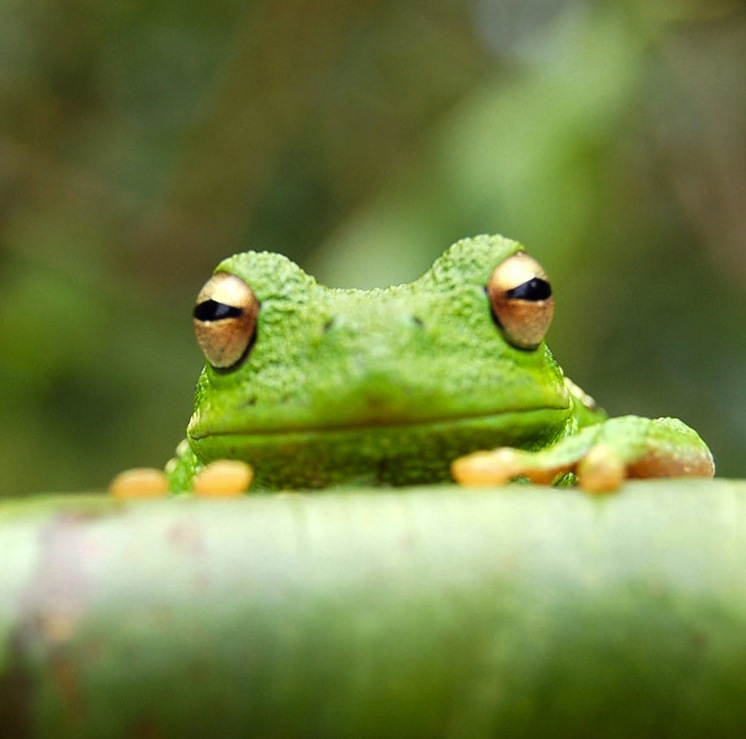
\includegraphics[width=6cm]{frog}}\label{figsupp:sf1}
\figsupp{This is another supplementary figure.}{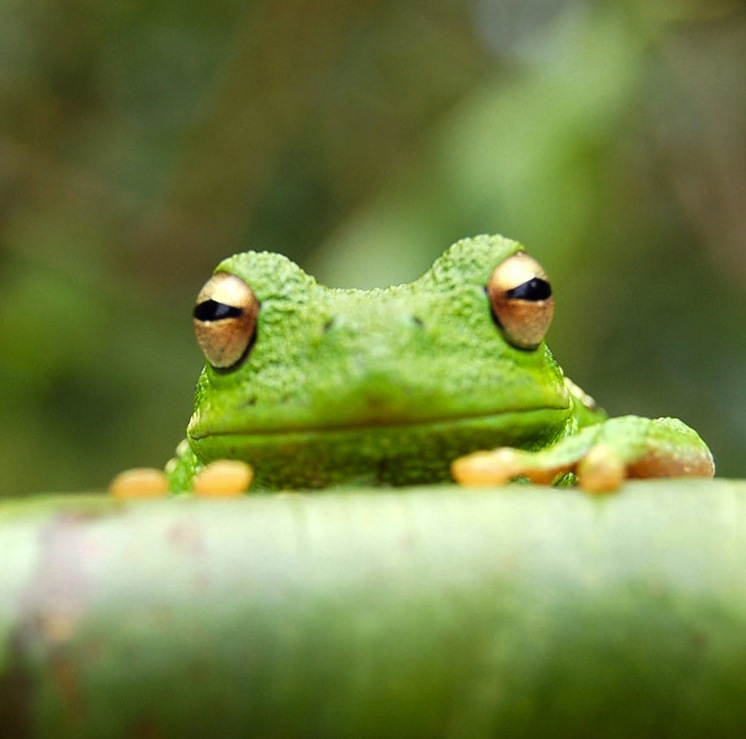
\includegraphics[width=6cm]{frog}}
\videosupp{This is a description of a video supplement.}\label{videosupp:sv1}
\figdata{This is a description of a data source.}\label{figdata:first}
\figdata{This is another description of a data source.}\label{figdata:second}
\end{figure}

\subsection{Comparison of Bayesisan method with heuristic spot thresholding}

We have done two types of performance comparison between the Bayesian method and the heuristic spot thresholding method. For the first performance comparison, a series of simulated data sets was constructed for a range of signal-to-noise values. For each S/N, a set of images with and without a 2-D Gaussian spots bound at the target and off-target were randomly generated. Intensity noise was generated using Gamma distribution to all simulated images.

Each data set was analyzed by both the Bayesian method and the heuristic spot thresholding algorithm (e.g., Figure 2, left). By comparison with the known “true” identities of the images, the accuracy of the resulting classifications was judged using a variety of specialized statistics for binary classification data, including true and false positive rates, true and false negative rates, and the Matthews Correlation Coefficient (MCC) \citep{fawcett_introduction_2006, matthews_comparison_1975}. The MCC statistic is widely regarded as a single overall, balanced measure which is meaningful even when the classes are of very different sizes. The MCC corresponds to the Pearson correlation coefficient between the estimated and “true” binary classifications. MCC=+1 represents a perfect prediction, MCC=0 a perfectly random prediction, and MCC=-1 indicates maximal disagreement between truth and estimation.

In a second comparison, images from real (i.e., not simulated) experimental data recordings were analyzed (Figure 3). Over a range of S/N, the Bayesian method gave image classification accuracy (as quantified by the MCC) similar to (or possibly better than) the heuristic spot thresholding algorithm The Bayesian method performs as well as the best existing CoSMoS data analysis method. Furthermore, Bayesian method achieves this performance automatically, with no adjustable parameters whatsoever, unlike the heuristic spot picker which attains this level of performance only after careful subjective trial-and-error manual adjustment of its three threshold parameters, a process that must be repeated tediously for each data set analyzed. Finally, our new Bayesian method produces a spot probability estimate for each image (not merely a Boolean spot/no spot determination) that can be used to inform subsequent kinetics calculations based on the results (e.g., the HMM analysis).

\subsection{Probabilistic modeling based on fundamental statistical analysis of data and priors}

To solve the problems with existing CoSMoS data analysis methods identified above, we have developed a new image-analysis-based approach that is accurate, objective, and built on a rigorous statistical approach to the CoSMoS image analysis problem. This TIBSD method is based on probabilistic modeling methodology. Bayesian model is a statistical model where probability is used to represent all uncertainty within the model, both for observed and hidden quantities in a system of interest. Bayes' theorem allows to perform inference on hidden variables given the observed data. The proposed first use of these methods for CoSMoS allows straightforward estimates of the uncertainty for estimated model parameters and rigorous quantitative testing of alternative image, noise, and kinetic models. “Time-independent” in the name TIBSD indicates that we ignore the time dimension of the recording -- the order of the images is arbitrary and does not affect the model, as each image is considered statistically independent of the others. We note that this time-independent method can naturally be extended into a time-dependent approach to both more accurately analyze the images and to directly obtain information about molecular kinetic mechanisms.  The proposed methods will eliminate the need for subjective image inspection and minimize the manual work required for CoSMoS data analysis.

\subsection{Time-independent Bayesian Spot Discrimination (TIBSD) method for analysis of CoSMoS data}

Unlike standard analysis methods for CoSMoS and single molecule FRET (smFRET), which are based on scalar intensity measurements derived from integration of emission in image regions of interest, our model fully uses information contained in the raw two-dimensional microscope images. The value of image data is proven in previous studies (Larry, Grunwald). To analyze the CoSMoS image classification problem within a Bayesian framework, one must define ideal image shapes for each class (image model) and choose a likelihood function for the observed data (noise model).

\subsubsection{Image classification}

The CoSMoS data set consists of a set of images where we have $N$ target sites ($n \in \{1,\dots,N\}$) each consisting of a series of $F$ different images in a recording ($f \in \{1,\dots,F\}$) (a “recording”). In each image, a binder molecule is either present on the single target molecule or absent. In addition, we explicitly model off-target binding of binder molecule. For simplicity  we assume that experimental conditions and image size were chosen so that at most only two spots ($K=2$) can exist in one image ($m_{nfk} \in \{ 0,1 \}$ -- existence indicator of the $k$-th spot). We treat the image classification problem as a data association problem by introducing an index variable for the on-target spot ($\theta_{nf} \in \{ 0,1,\dots,K \}$) where 0 means that on-target molecule is absent.

\subsubsection{Image model}

In the TIBSD method, we model the observed image data as a mixture of background image and “spot” images of binder molecules superimposed on background image. In particular, background image is modeled as a constant average background intensity $b_{nf}$; each spot image (2D point spread function) is modelled as an ideal (i.e., noiseless) 2-D Gaussian spot with integrated scalar intensity $h_{nfk}$ centered at ($x_{nfk}, y_{nfk}$). Each image is represented as a matrix (2D-array) $\mu^D_{nfij}$ of $P \times P$ pixels ($i,j \in \{1,\dots,P\}$). 

\textbf{\begin{equation*}
    \mu^{D}_{nfij} = b_{nf} + \sum_{k=1}^{K} \dfrac{m_{nfk}h_{nfk}}{2 \pi w^2_{nfk}} \exp{\left ( -\dfrac{(i-x_{nfk})^2 + (j-y_{nfk})^2}{2w^2_{nfk}} \right)}
\end{equation*}}

\subsubsection{Noise model}

 We use Gamma distribution as a noise model which is more flexible than Gaussian noise and can better approximate Poissonian camera noise. Scale parameter [add the variable name here?] of the Gamma distribution can be interpreted as a camera gain. Thus, the likelihood for the observed image can be expressed as:
 
 \begin{equation*}
     p(D_{nf}|\mu^D_{nfij},gain) = Gamma(D_{nf}|\mu^D_{nfij}/gain,1/gain)
 \end{equation*}

\subsubsection{Prior knowledge of colocalization accuracy}

Prior knowledge of colocalization accuracy can be directly incorporated into our model as priors for the center of the spot. On-target spots are localized around the target molecule within the experimentally determined accuracy and off-target spots are uniformly distributed within the image:

\begin{equation*}
    x_{nfk} \sim
\begin{cases}
    Beta^{\prime}(x_{nfk}|\mu^x=0,\nu^x_{prox}),& \text{if } \theta = k\\
    Beta^{\prime}(x_{nfk}|\mu^x=0,\nu^x_{flat}),& \text{otherwise}
\end{cases}
\end{equation*}

\begin{equation*}
    y_{nfk} \sim
\begin{cases}
    Beta^{\prime}(y_{nfk}|\mu^y=0,\nu^y_{prox}),& \text{if } \theta = k\\
    Beta^{\prime}(y_{nfk}|\mu^y=0,\nu^y_{flat}),& \text{otherwise}
\end{cases}
\end{equation*}


%\subsection{Image analysis, probabilities not binary classification}

%Expresses uncertainty. Allows downstream analysis. 

%\subsection{Flexible framework. Can select and use different models depending on the experiment}

%\subsubsection{Ability to jointly analyze different experimental conditions}

%\subsubsection{Models easily expandable to incorporate other data features}

\subsection{Software and hardware implementation}

The proposed research will provide more efficient ways to analyze large CoSMoS data sets. Technological developments such as faster, larger cameras \citep{huang_particle_nodate}, availability of fluorescent dyes with dramatically improved photostability (which increase the amount of data from a single experiment), and microscopes that efficiently collect single-molecule data at more wavelengths simultaneously \citep{friedman_viewing_2006} have all increased the sizes of CoSMoS datasets. Gelles lab studies of transient molecular binding events at high frame rates have produced >1 TB image data per experiment. Increasing data set sizes make it infeasible to use existing analytical methods. The code for the model and variational inference algorithm is written using Pyro probabilistic programming language. Pyro uses Pytorch as a backend for automatic differentiation and efficient computation of parallelizable vector-math operations on graphics processing units (GPUs). Our program is open-source and can be downloaded from the github repository.

\begin{comment}
\begin{table}[bt]
\caption{\label{tab:example}Automobile Land Speed Records (GR 5-10).}
% Use "S" column identifier to align on decimal point 
\begin{tabular}{S l l l r}
\toprule
{Speed (mph)} & Driver          & Car                        & Engine    & Date     \\
\midrule
407.447     & Craig Breedlove & Spirit of America          & GE J47    & 8/5/63   \\
413.199     & Tom Green       & Wingfoot Express           & WE J46    & 10/2/64  \\
434.22      & Art Arfons      & Green Monster              & GE J79    & 10/5/64  \\
468.719     & Craig Breedlove & Spirit of America          & GE J79    & 10/13/64 \\
526.277     & Craig Breedlove & Spirit of America          & GE J79    & 10/15/65 \\
536.712     & Art Arfons      & Green Monster              & GE J79    & 10/27/65 \\
555.127     & Craig Breedlove & Spirit of America, Sonic 1 & GE J79    & 11/2/65  \\
576.553     & Art Arfons      & Green Monster              & GE J79    & 11/7/65  \\
600.601     & Craig Breedlove & Spirit of America, Sonic 1 & GE J79    & 11/15/65 \\
622.407     & Gary Gabelich   & Blue Flame                 & Rocket    & 10/23/70 \\
633.468     & Richard Noble   & Thrust 2                   & RR RG 146 & 10/4/83  \\
763.035     & Andy Green      & Thrust SSC                 & RR Spey   & 10/15/97\\
\bottomrule
\end{tabular}

\medskip 
Source: \url{https://www.sedl.org/afterschool/toolkits/science/pdf/ast_sci_data_tables_sample.pdf}

\tabledata{This is a description of a data source.}

\end{table}
\end{comment}

% wc 790
\section{Discussion}

\lipsum[9]

\section{Materials and Methods}

\subsection{Notation} 

In the Materials and Methods section, we adopt a mathematical notation for multi-dimensional arrays from the field of machine learning  \citep{Chiang2021-fi}.  The notation uses \textit{named axes} and incorporates implicit broadcasting of arrays when their shapes are different.

\subsection{Extracting image data} 

Raw input data into Tapqir consists of 1) binder channel images ($D^\mathsf{raw}$), each $W \times H$ pixels in size, for each time point (\FIG{cosmos_experiment}B, right), and 2)  lists of locations, corrected for microscope drift if necessary \citep{Friedman2015-nx}, of target molecules and of off-target control locations  \citep{Friedman2015-nx} within the raw images. For simplicity we use the same notation ($x^{\mathsf{target}, \mathsf{raw}}$, $y^{\mathsf{target}, \mathsf{raw}}$) both for target molecule locations and off-target control locations. Tapqir extracts a $P \times P$ AOI around each target and off-target location and returns 1) the extracted data set $D$ consisting of a set of $P \times P$ grayscale images, collected at $N$ on-target AOI sites and $N_\mathsf{c}$  off-target AOI sites for a range of $F$ frames (\FIG{cosmos_experiment}C,D; \ALGORITHM{preprocessing}), and 2) new target (and off-target) locations ($x^\mathsf{target}$, $y^\mathsf{target}$) adjusted relative to extracted images $D$ where $x^\mathsf{target}$ and $y^\mathsf{target}$ both lie within the $(P/2-1,P/2)$ central range of the image. For the data presented in this article, we used $P = 14$. Cartesian pixel indices ($i$, $j$) are integers but also represent the center point of a pixel on the image plane. While experimental intensity measurements are integers, we treat them as continuous values in our analysis.

\algnewcommand{\LineComment}[1]{\State \(\triangleright\) #1}

\paragraph{Algorithm 1.} Extraction of AOI images from raw images. \\

\begin{algorithmic}[1]
\State \textbf{input:} $D^\mathsf{raw}$, $x^{\mathsf{target},\mathsf{raw}}$, $y^{\mathsf{target},\mathsf{raw}}$
\ForAll{$\mathsf{frame}[F]$}
    \ForAll{$\mathsf{AOI}[N]$}
        \LineComment{$(P-1)/2$ is an AOI image center}
        \LineComment{$\mathsf{round}$ function rounds to the closest integer}
        \State $\mathsf{shiftX} = \mathsf{round} \left( x^{\mathsf{target},\mathsf{raw}} - (P - 1) / 2 \right) $
        \State $\mathsf{shiftY} = \mathsf{round} \left( y^{\mathsf{target},\mathsf{raw}} - (P - 1) / 2 \right) $
        \State $x^\mathsf{target} = x^{\mathsf{target}, \mathsf{raw}} - \mathsf{shiftX}$
        \State $y^\mathsf{target} = y^{\mathsf{target}, \mathsf{raw}} - \mathsf{shiftY}$
        \State $D_{\mathsf{AOI}(n), \mathsf{pixelX}(i), \mathsf{pixelY}(j)} = D^{\mathsf{raw}}_{\mathsf{pixelX}(i+\mathsf{shiftX}_{\mathsf{AOI}(n)}), \mathsf{pixelY}(j+\mathsf{shiftY}_{\mathsf{AOI}(n)})}$
        %\State $D_{\mathsf{AOI}(n), \mathsf{frame}(f), \mathsf{pixelX}(i), \mathsf{pixelY}(j)} = D^{\mathsf{raw}}_{\mathsf{frame}(f), \mathsf{pixelX}(i+\mathsf{shiftX}_{\mathsf{AOI}(n), \mathsf{frame}(f)}), \mathsf{pixelY}(j+\mathsf{shiftY}_{\mathsf{AOI}(n), \mathsf{frame}(f)})}$
    \EndFor
\EndFor
\Return $D$, $x^\mathsf{target}$, $y^\mathsf{target}$
\end{algorithmic}

\subsection{The \emph{cosmos} model} 

Our intent is to model CoSMoS image data by accounting for the significant physical aspects of image formation, such as photon noise and binding of target-specific and target-nonspecific molecules to the microscope slide surface. A graphical representation of the Tapqir model for CoSMoS data similar to that in \FIG{graphical_model}D but including probability distributions and other additional detail is shown in \FIGSUPP[graphical_model]{extended}. The corresponding generative model represented as pseudocode is shown in \ALGORITHM{model}. All variables with short descriptions and their domains are listed in \TABLE{variables}. Below, we describe the model in detail starting with the observed data and the likelihood function and then proceed with model parameters and their prior distributions.

\subsubsection{Image likelihood}

We model the image data $D$ as the sum of a photon-independent offset $\delta$ introduced by the camera and the noisy photon-dependent pixel intensity values $I$:
%
\begin{equation}
    D = \delta + I
\end{equation}

In our model, each pixel in the photon-dependent image $I$ has a  variance which is equal to  the mean intensity $\mu^I$ of that pixel multiplied by the camera gain $g$, which is the number of camera intensity units per photon. This formulation is appropriate for cameras that use charge-coupled device (CCD) or electron-multiplier CCD (EMCCD) sensors.  (The experimental CoSMoS datasets we analyzed (\TABLE{datasets}) were collected with EMCCD cameras.)  It accounts for both photon shot noise and additional noise introduced by EMCCD camera amplification \citep{Van_Vliet1998-jk} and is expressed using a continuous Gamma distribution:
%
\begin{equation}
    I \sim \mathbf{Gamma} (\mu^I, \sqrt{\mu^I \cdot g})
\end{equation}

The Gamma distribution was chosen because we found it to effectively model the image noise, which includes both Poissonian (shot noise) and non-Poissonian contributions. The Gamma distribution used here is parameterized by its mean and standard deviation. The functional forms of the Gamma distribution and all other distributions we use in this work are given in \TABLE{distributions}.

A competing camera technology based on scientific complementary metal-oxide semiconductor (sCMOS) sensors produces images that have also successfully been modeled as having a combination of Poissonian and non-Poissonian (Gaussian, in this case) noise sources. However, sCMOS images have noise characteristics that are considerably more complicated than CCD/EMCCD images, because every pixel has its own characteristic intensity offset, Gaussian noise variance, and amplification gain. Additional validation will be required to determine whether the existing \emph{cosmos} model requires modification or inclusion of additional prior information (e.g., pixel-by-pixel calibration data as in \cite{Huang2013-bx}) to optimize its performance with sCMOS CoSMoS data.

\subsubsection{Image model}

The idealized noise-free image $\mu^I$ is represented  as the sum of a background intensity $b$ and the intensities from fluorescence spots modeled as  2-D Gaussians $\mu^S$:
%
\begin{equation}
    \mu^I = b + \sum_{\mathsf{spot}} \mu^S
\end{equation}

\noindent
For simplicity we allow at most $K$ number of spots in each frame of each AOI.  (In this article, we always use $K$ equal to 2.)  The presence of a given spot in the image is encoded in the binary spot existence parameter $m$, where $m = 1$ when the corresponding spot is present and $m = 0$ when it is absent.

The intensities for a 2-D Gaussian spot at each pixel coordinate ($i$, $j$) is given by:
%
\begin{equation}
    \mu^S_{\mathsf{pixelX}(i), \mathsf{pixelY}(j)} = \dfrac{m \cdot h}{2 \pi w^2} \exp{\left( -\dfrac{(i-x-x^\mathsf{target})^2 + (j-y-y^\mathsf{target})^2}{2 w^2} \right)}
\end{equation}

\noindent
with spot parameters total integrated intensity $h$, width $w$, and center ($x$, $y$) relative to the target (or off-target control) location ($x^\mathsf{target}$, $y^\mathsf{target}$). 
%

Our primary interest is whether a target-specific spot is absent or present in a given AOI. We encode this information using a binary \emph{state} parameter $z$ with 0 and 1 denoting target-specific spot absence and presence, respectively. To indicate which of the $K$ spots is target-specific, we use the \emph{index} parameter $\theta$ which ranges from $0$ to $K$. When a target-specific spot is present ($z = 1$), $\theta \in \{1, \cdots, K \}$ specifies the index of the target-specific spot, while $\theta = 0$ indicates that no target-specific spot is present ($z = 0$). For example, $\{ m_{\mathsf{spot}(1)}=1, m_{\mathsf{spot}(2)}=1, z = 1, \theta=2 \}$ means that both spots are present and spot 2 is target-specific. A combination like $\{ m_{\mathsf{spot}(1)}=0, m_{\mathsf{spot}(2)}=1, z = 1, \theta=1 \}$ is impossible (i.e, has zero probability) since spot 1 cannot be absent and target-specific at the same time. For off-target control data, in which no spots are target-specific by definition, $z$ and $\theta$ are always set to zero.
%

\subsubsection{Prior distributions}

The prior distributions for the model parameters are summarized in \FIGSUPP[graphical_model]{extended} and detailed below. Unless otherwise indicated we assume largely uninformative priors (such as the Half-Normal distribution with large mean). 

Background intensity $b$ follows a Gamma distribution:
%
\begin{equation}
    b \sim \mathbf{Gamma}(\mu^b, \sigma^b)
\end{equation}

\noindent
where the mean $\mu^b \in \mathbb{R}_{>0}^{\mathsf{AOI}[N]}$ and standard deviation $\sigma^b \in \mathbb{R}_{>0}^{\mathsf{AOI}[N]}$ of the background intensity describe the irregularity in the background intensity in time and across the field of view of the microscope. Priors for $\mu^b$ and $\sigma^b$ are uninformative:
%
\begin{subequations}
\begin{align}
    \mu^b &\sim \mathbf{HalfNormal}(1000) \\
    \sigma^b &\sim \mathbf{HalfNormal}(100)
\end{align}
\end{subequations}
%
The target-specific presence parameter $z$ has a Bernoulli prior parameterized by the average target-specific binding probability $\pi \in [0, 1] $ for on-target AOIs and zero probability for control off-target AOIs:
%
\begin{equation}
    z \sim
    \begin{cases}
        \mathbf{Bernoulli}(\pi) & \text{on-target AOI} \\
        0 & \text{control off-target AOI} \rule{0pt}{4ex}
    \end{cases}
\end{equation}
%
The prior distribution for the index of the target-specific spot $\theta$ is conditional on $z$. When no specifically bound spot is present (i.e., $z = 0$) $\theta$ always equals 0. Since spot indices are arbitrarily assigned, when the target-specific spot is present (i.e., $z = 1$) $\theta$ can take any value between $1$ and $K$ with equal probability. We represent the prior for $\theta$ as a Categorical distribution of the following form:
%
\begin{equation}
    \theta \sim
    \begin{cases}
        0 & z = 0 \\
        \mathbf{Categorical}\left( \begin{bmatrix} 0, \frac{1}{K}, \dots, \frac{1}{K} \end{bmatrix} \right) & z = 1 \rule{0pt}{4ex}
    \end{cases}
\end{equation}

The average target-specific binding probability $\pi$ has an uninformative Jeffreys prior \citep{Gelman2013-ro} given by a Beta distribution:
%
\begin{equation}
    \pi \sim \mathbf{Beta}(1/2, 1/2)
\end{equation}

The prior distribution for the spot presence indicator $m$ is conditional on $\theta$. When $\theta$ corresponds to spot index $k$, i.e., $\theta = k$, then $m_{\mathsf{spot}(k)} = 1$. When $\theta$ does not correspond to a spot index $k$, i.e., $\theta \neq k$, then either spot $k$ is target-nonspecific or a spot corresponding to $k$ does not exist. Consequently, for $\theta \neq k$ we assign $m_{\mathsf{spot}(k)}$ to either 0 or 1 with a probability dependent on the non-specific binding density $\lambda \in \mathbb{R}_{>0}$:
%
\begin{equation}
    m_{\mathsf{spot}(k)} \sim
    \begin{cases}
        1 & \text{$\theta = k$} \\
        \mathbf{Bernoulli} \left( \sum_{l=1}^K \dfrac{l \cdot \mathbf{TruncPoisson}(l; \lambda, K)}{K} \right) & \text{$\theta = 0$} \rule{0pt}{4ex} \\
        \mathbf{Bernoulli} \left( \sum_{l=1}^{K-1} \dfrac{l \cdot \mathbf{TruncPoisson}(l; \lambda, K-1)}{K-1} \right) & \text{otherwise} \rule{0pt}{4ex}
    \end{cases}
\end{equation}

The mean non-specific binding density $\lambda$ is expected to be much less than two non-specifically bound spots per frame per AOI; therefore, we use an Exponential prior of the form
%
\begin{equation}
    \lambda \sim \mathbf{Exponential}(1)
\end{equation}

The prior distribution for the integrated spot intensity $h$ is chosen to fall off at a value much greater than typical spot intensity values 
%
\begin{equation}
    h \sim \mathbf{HalfNormal}(10000)
\end{equation}

In CoSMoS experiments the microscope/camera hardware is typically designed to set the width $w$ of fluorescence spots to a  typical value in the range of 1--2 pixels \citep{Ober2015-ba}. We use a Uniform prior confined to the range between 0.75 and 2.25 pixels:
%
\begin{equation}
    w \sim \mathbf{Uniform}(0.75, 2.25)
\end{equation}

Priors for spot position ($x$, $y$) depend on whether the spot represents target-specific or non-specific binding. Non-specific binding to the microscope slide surface can occur anywhere within the image and therefore has a uniform distribution (\FIGSUPP[graphical_model]{xy}, red). Spot centers may fall slightly outside the AOI image yet still affect pixel intensities within the AOI.  Therefore the range for ($x$, $y$) is extended one pixel wider than the size of the image, which allows a spot center to fall slightly beyond the AOI boundary.

In contrast to non-specifically bound molecules, specifically bound molecules are colocalized with the target molecule with a precision that can be smaller than one pixel and that depends on various factors including the microscope point-spread function and magnification, accuracy of registration between binder and target image channels, and accuracy of drift correction. For target-specific binding, we use an Affine-Beta prior with zero mean position relative to the target molecule location ($x^\mathsf{target}$, $y^\mathsf{target}$), and a ``proximity'' parameter $\sigma^{xy}$ which is the  standard deviation of the AffineBeta distribution (\FIGSUPP[graphical_model]{xy}, green). We chose the Affine-Beta distribution because it models a continuous parameter defined on a bounded interval.
%
\begin{equation}
    x_{\mathsf{spot}(k)}, y_{\mathsf{spot}(k)} \sim
    \begin{cases}
        \mathbf{AffineBeta}\left( 0, \sigma^{xy}, -\dfrac{P+1}{2}, \dfrac{P+1}{2} \right) & \theta = k ~\text{(target-specific)} \\
        \mathbf{Uniform}\left(-\dfrac{P+1}{2}, \dfrac{P+1}{2} \right) & \theta \neq k ~\text{(target-nonspecific)} \rule{0pt}{4ex}
    \end{cases}
\end{equation}

We give the proximity parameter $\sigma^{xy}$ a diffuse prior, an Exponential with a characteristic width of one pixel:
%
\begin{equation}
    \sigma^{xy} \sim \mathbf{Exponential}(1)
\end{equation}

Tests on data simulated with increasing proximity parameter values $\sigma^{xy}$ (true) (i.e., with decreasing precision of spatial mapping between the binder and target image channels) confirm that the \emph{cosmos} model accurately learns  $\sigma^{xy}$ (fit) from the data  (\FIGSUPP[tapqir_analysis]{randomized}D; \TABLE{proximity}).  This was the case even if we substituted a less-informative $\sigma^{xy}$ prior (Uniform vs. Exponential; \TABLE{proximity}).

The CoSMoS technique is premised on colocalization of the binder spots with the known location of the target molecule.  Consequently, for any analysis method, classification accuracy declines when the images in the target and binder channels are less accurately mapped.  For the Tapqir \emph{cosmos} model, low mapping precision has little effect on classification accuracy at typical non-specific binding densities ($\lambda = 0.15$; see MCC values in \TABLE{proximity}).

Gain $g$ depends on the settings of the amplifier and electron multiplier (if present) in the camera. It has a positive value and is typically in the range between 5--50. We use a Half-Normal prior with a broad distribution encompassing this range:
%
\begin{equation}
    g \sim \mathbf{HalfNormal}(50)
\end{equation}

The prior distribution for the offset signal $\delta$ is empirically measured from the output of camera sensor regions that are masked from incoming photons. Collected data from these pixels are transformed into a density histogram with intensity step size of 1. The resulting histogram typically has a long right hand tail of low density. For computational efficiency, we shorten this tail by binning together pixel intensity values from the upper 0.5\% percentile. Since $D = \delta + I$ (Eq. 1) and photon-dependent intensity $I$ is positive, all $D$ values have to be larger than the smallest offset intensity value. If that is not the case we add a single value $\min(D) - 1$ to the offset empirical distribution which has a negligible effect on the distribution. Bin values $\delta_\mathsf{samples}$ and their weights $\delta_\mathsf{weights}$ are used to construct an Empirical prior:
%
\begin{equation}
    \delta \sim \mathbf{Empirical}(\delta_\mathsf{samples}, \delta_\mathsf{weights})
\end{equation}

All simulated and experimental data sets in this work were analyzed using the prior distributions and hyperparameter values given above, which are compatible with a broad range of experimental conditions (\TABLE{datasets}). Many of the priors are uninformative  and we anticipate that these will work well with images taken on variety of microscope hardware.  However, it is possible that highly atypical microscope designs (e.g., those with effective magnifications that are sub-optimal for CoSMoS) might require adjustment of some fixed hyperparameters and distributions (those in Eqs. 6a, 6b, 11, 12, 13, 15, and 16). For example, if the microscope point spread function is more than 2 pixels wide, it may be necessary to increase the range of the $w$ prior in Eq. 13.  The Tapqir documentation (\url{https://tapqir.readthedocs.io/en/stable/}) gives instructions for changing the hyperparameters.

\subsection{Joint distribution}

The joint distribution of the data and all parameters is the fundamental distribution necessary to perform a Bayesian analysis.  Let $\phi$ be the set of all model parameters. The joint distribution can be expressed in a factorized form:
%
\begin{equation}
\begin{aligned}
    p(D, \phi) =~&p(g) p(\sigma^{xy}) p(\pi) p(\lambda) \prod_{\mathsf{AOI}} \left[ p(\mu^b) p(\sigma^b) \prod_{\mathsf{frame}} \left[ \vphantom{\prod_{F}} p(b | \mu^b, \sigma^b) p(z | \pi) p(\theta | z) \vphantom{\prod_{\substack{\mathsf{pixelX} \\ \mathsf{pixelY}}}} \cdot \right. \right. \\
    &\prod_{\mathsf{spot}} \left[ \vphantom{\prod_{F}} p(m | \theta, \lambda) p(h) p(w) p(x | \sigma^{xy}, \theta) p(y | \sigma^{xy}, \theta) \right] \left. \left. \prod_{\substack{\mathsf{pixelX} \\ \mathsf{pixelY}}} p(\delta) p(D | \mu^I, g, \delta) \right] \right]
\end{aligned}
\end{equation}

The Tapqir generative model is a stochastic function that describes a properly normalized joint distribution for the data and all parameters (\ALGORITHM{model}). In Pyro this is called ``the model''.
 
\paragraph{Algorithm 2.} The Tapqir generative model is a stochastic function that describes a properly normalized joint distribution for the data and all parameters. In Pyro this is called ``the model''. \\

\begin{algorithmic}[1]
\State $g \sim \mathbf{HalfNormal}(50)$
\Comment{camera gain}
\State $\sigma^{xy} \sim \mathbf{Exponential}(1)$
\Comment{std of on-target spot position (pixels)}
\State $\pi \sim \mathbf{Beta}(1/2, 1/2)$
\Comment{average specific binding probability}
\State $\lambda \sim \mathbf{Exponential}(1)$
\Comment{non-specific binding rate}
\ForAll{$\mathsf{AOI}[N+N_\mathsf{c}]$}
    \State $\mu^b \sim \mathbf{HalfNormal}(1000)$
    \Comment{mean background intensity}
    \State $\sigma^b \sim \mathbf{HalfNormal}(100)$
    \Comment{std of background intensity}
    \ForAll{$\mathsf{frame}[F]$}
        \State $b \sim \mathbf{Gamma}(\mu^b, \sigma^b)$
        \Comment{background intensity}
        \If{on-target AOI}
            \State $\theta \sim \mathbf{Categorical}\left(1 - \pi, \frac{\pi}{K}, \dots, \frac{\pi}{K}\right)$
            \Comment{target-specific spot index}
        \ElsIf{off-target AOI}
            \State $\theta = 0$
        \EndIf
        \ForAll{$\mathsf{spot}[K]$}
            \State $ m_{\mathsf{spot}(k)} \sim
                \begin{cases}
                    \mathbf{Bernoulli}(1) & \text{$\theta = k$} \\
                    \mathbf{Bernoulli} \left( \sum_{l=1}^K \dfrac{l \cdot \mathbf{TruncPoisson}(l; \lambda, K)}{K} \right) & \text{$\theta = 0$} \\
                    \mathbf{Bernoulli} \left( \sum_{l=1}^{K-1} \dfrac{l \cdot \mathbf{TruncPoisson}(l; \lambda, K-1)}{K-1} \right) & \text{otherwise}
                \end{cases} $
            \Comment{spot presence}
            \State $h \sim \mathbf{HalfNormal}(10000)$
            \Comment{spot intensity}
            \State $w \sim \mathbf{Uniform}(0.75, 2.25)$
            \Comment{spot width}
            \State $ x_{\mathsf{spot}(k)} \sim
                \begin{cases}
                \mathbf{AffineBeta}\left( 0, \sigma^{xy}, -\dfrac{P+1}{2}, \dfrac{P+1}{2} \right) & \theta = k \\
                \mathbf{Uniform}\left(-\dfrac{P+1}{2}, \dfrac{P+1}{2} \right) & \theta \neq k \end{cases} $
            \Comment{$x$-axis center}
            \State $ y_{\mathsf{spot}(k)} \sim
                \begin{cases}
                \mathbf{AffineBeta}\left( 0, \sigma^{xy}, -\dfrac{P+1}{2}, \dfrac{P+1}{2} \right) & \theta = k \\
                \mathbf{Uniform}\left(-\dfrac{P+1}{2}, \dfrac{P+1}{2} \right) & \theta \neq k \end{cases}
                $
            \Comment{$y$-axis center}
            \ForAll{$\mathsf{pixelX}[P] \times \mathsf{pixelY}[P]$}
            \State $\mu^{S}_{\mathsf{pixelX}(i), \mathsf{pixelY}(j)} =
                        \dfrac{m \cdot h}{2 \pi w^2} \exp{\left ( -\dfrac{(i-x-x^\mathsf{target})^2 + (j-y-y^\mathsf{target})^2}{2w^2} \right)}$
            \Comment{2-D Gaussian spot}
            \EndFor
        \EndFor
            
        \ForAll{$\mathsf{pixelX}[P] \times \mathsf{pixelY}[P]$}
            \State $\delta \sim \mathbf{Empirical}( \delta_\mathsf{samples}, \delta_\mathsf{weights})$
            \Comment{offset signal}
            \State $\mu^I = b + \sum_{\mathsf{spot}} \mu^S$
            \Comment{mean pixel intensity w/o offset}
            \State $I \sim \mathbf{Gamma} (\mu^I, \sqrt{\mu^I \cdot g})$
            \Comment{pixel intensity w/o offset}
            \State $D = \delta + I$
            \Comment{observed pixel intensity}
        \EndFor
    \EndFor
\EndFor
\end{algorithmic}

\subsection{Inference}

For a Bayesian analysis, we want to obtain the posterior distribution for parameters $\phi$ given the observed data $D$. There are three discrete parameters $z$, $\theta$, and $\delta$ that can be marginalized out exactly so that they do not appear expilictly in either the joint posterior distribution or the likelihood function. Computationally efficient marginalization is implemented using Pyro's enumeration strategy \citep{Obermeyer2019-xt} and KeOps' kernel operations on the GPU without memory overflows \citep{Charlier2021-vq}. Let $\phi^{\prime} = \phi - \{ z, \theta, \delta \}$ be the rest of the parameters. We obtain posterior distributions of $\phi^{\prime}$ using Bayes' rule:
%
\begin{equation}
    p(\phi^{\prime} | D) =
    \dfrac{\sum_{z, \theta, \delta} p(D, \phi)}{\int_{\phi} p(D, \phi) d\phi} =
    \dfrac{p(D, \phi^{\prime})}{\int_{\phi} p(D, \phi) d\phi} =
    \dfrac{p(D| \phi^{\prime} )p(\phi^{\prime})}{\int_{\phi} p(D, \phi) d\phi}
\end{equation}

Note that the integral in the denominator of this expression is necessary to calculate the posterior distribution, but it is usually analytically intractable. However, variational inference provides a robust method to approximate the posterior distribution $p(\phi^{\prime} | D)$ with a parameterized variational distribution $q(\phi^{\prime})$ \citep{Bishop2006-oa}.
%
\begin{equation}
    p(\phi^{\prime} | D) \simeq q(\phi^{\prime})
\end{equation}


$q(\phi^{\prime})$ has the following factorization:

\begin{equation}
\begin{aligned}
    q(\phi^{\prime}) =~&q(g) q(\sigma^{xy}) q(\pi) q(\lambda) \cdot \\
    &\prod_{\mathsf{AOI}} \left[ q(\mu^b) q(\sigma^b) \prod_{\mathsf{frame}} \left[ q(b) \prod_{\mathsf{spot}} \left[ \vphantom{\prod_{F}} q(m) q(h | m) q(w | m) q(x | m) q(y | m) \right] \right] \right]
\end{aligned}
\end{equation}

The variational distribution $q(\phi^{\prime})$ is provided as pseudocode for a generative stochastic function (\ALGORITHM{guide}). In Pyro this is called ``the guide''. Variational inference is sensitive to initial values of variational parameters. In \ALGORITHM{guide}, step 1 we provide the initial values of variational parameters used in our analyses.

%\label{alg:pseudocode}
\paragraph{Algorithm 3.} Pseudocode representation of Tapqir guide.

\algnewcommand{\Initialize}[1]{%
  \State \textbf{Variational parameter initializations} $\{ \mathrm{initial\:value}, \quad \mathrm{constraint} \}$:
  \Statex \hspace*{\algorithmicindent}\parbox[t]{.8\linewidth}{\raggedright #1}
}

\begin{algorithmic}[1]
\Initialize{
    $g_\mathsf{mean} \gets \{ 5, \quad \mathbb{R}_{>0} \} $ \\
    $g_\mathsf{beta} \gets \{ 100, \quad \mathbb{R}_{>0} \} $ \rule{0pt}{3ex} \\
    $\sigma^{xy}_\mathsf{mean} \gets \{ 0, \quad (0, (P+1) / \sqrt{12}) \} \rule{0pt}{3ex} $ \\
    $\sigma^{xy}_\mathsf{beta} \gets \{ 100, \quad \mathbb{R}_{>2} \} $ \rule{0pt}{3ex} \\
    $\pi_\mathsf{mean} \gets \{ 0.5, \quad [0, 1] \} $ \rule{0pt}{3ex} \\
    $\pi_\mathsf{size} \gets \{ 2, \quad \mathbb{R}_{>2} \} $ \rule{0pt}{3ex} \\
    $\lambda_\mathsf{mean} \gets \{ 0.5, \quad \mathbb{R}_{>0} \} $ \rule{0pt}{3ex} \\
    $\lambda_\mathsf{beta} \gets \{ 100, \quad \mathbb{R}_{>0} \} $ \rule{0pt}{3ex} \\
    $\mu^b_\mathsf{mean} \gets \{ \mathsf{mean}(D)^{\mathsf{AOI}[N]}, \quad \mathbb{R}_{>0} \}$ \rule{0pt}{3ex} \\
    $\sigma^b_\mathsf{mean} \gets \{ 1^{\mathsf{AOI}[N]}, \quad \mathbb{R}_{>0} \}$ \rule{0pt}{3ex} \\
    $b_\mathsf{mean} \gets \{ \mathsf{mean}(D)^{\mathsf{AOI}[N] \times \mathsf{frame}[F]}, \quad \mathbb{R}_{>0} \}$ \rule{0pt}{3ex} \\
    $b_\mathsf{beta} \gets \{ 1^{\mathsf{AOI}[N] \times \mathsf{frame}[F]}, \quad \mathbb{R}_{>0} \} $ \rule{0pt}{3ex} \\
    $\theta_\mathsf{prob} \gets \{ 1/3^{\mathsf{target}[1+K] \times \mathsf{AOI}[N] \times \mathsf{frame}[F]}, \quad \sum_\mathsf{target} \theta_\mathsf{prob} = 1 \}$ \rule{0pt}{3ex} \\
    $m_\mathsf{prob} \gets \left\{ \mathsf{target} \begin{array}[b]{@{}c@{}}\mathsf{spot}\\\begin{bmatrix} 0.5 & 0.5 \\ 1 & 0.5 \\ 0.5 & 1 \end{bmatrix}\end{array}^{\mathsf{AOI}[N] \times \mathsf{frame}[F]}, \quad [ 0, 1 ] \right \} $ \rule{0pt}{3ex} \\
    $h_\mathsf{mean} \gets \{ 2000^{\mathsf{spot}[K] \times \mathsf{AOI}[N] \times \mathsf{frame}[F]}, \quad \mathbb{R}_{>0} \} $ \rule{0pt}{3ex} \\
    $h_\mathsf{beta} \gets \{ 0.001^{\mathsf{spot}[K] \times \mathsf{AOI}[N] \times \mathsf{frame}[F]}, \quad \mathbb{R}_{>0} \} $ \rule{0pt}{3ex} \\
    $w_\mathsf{mean} \gets \{ 1.5^{\mathsf{spot}[K] \times \mathsf{AOI}[N] \times \mathsf{frame}[F]}, \quad [0.75, 2.25] \} $ \rule{0pt}{3ex} \\
    $w_\mathsf{size} \gets \{ 100^{\mathsf{spot}[K] \times \mathsf{AOI}[N] \times \mathsf{frame}[F]}, \quad \mathbb{R}_{>2} \} $ \rule{0pt}{3ex} \\
    $x_\mathsf{mean} \gets \{ 0^{\mathsf{spot}[K] \times \mathsf{AOI}[N] \times \mathsf{frame}[F]}, \quad [-(P+1)/2, (P+1)/2] \} $ \rule{0pt}{3ex} \\
    $y_\mathsf{mean} \gets \{ 0^{\mathsf{spot}[K] \times \mathsf{AOI}[N] \times \mathsf{frame}[F]}, \quad [-(P+1)/2, (P+1)/2] \} $ \rule{0pt}{3ex} \\
    $xy_\mathsf{size} \gets \{ 200^{\mathsf{spot}[K] \times \mathsf{AOI}[N] \times \mathsf{frame}[F]}, \quad \mathbb{R}_{>2} \} $ \rule{0pt}{3ex}
    }
\State $g \sim \mathbf{Gamma}(g_\mathsf{mean}, \sqrt{g_\mathsf{mean} / g_\mathsf{beta}})$
\Comment{camera gain}
\State $\sigma^{xy} \sim \mathbf{AffineBeta}(\sigma^{xy}_\mathsf{mean}, \sigma^{xy}_\mathsf{size}, 0, (P+1) / \sqrt{12})$
\Comment{std of on-target spot position (pixels)}
\State $\pi \sim \mathbf{Beta}(\pi_\mathsf{mean}, \pi_\mathsf{size})$
\Comment{average specific binding probability}
\State $\lambda \sim \mathbf{Gamma}(\lambda_\mathsf{mean}, \sqrt{\lambda_\mathsf{mean} / \lambda_\mathsf{beta}})$
\Comment{non-specific binding rate}
\ForAll{$\mathsf{AOI}[N+N_\mathsf{c}]$}
    \State $\mu^b \sim \mathbf{Delta}(\mu^b_\mathsf{mean})$
    \Comment{mean background intensity} 
    \State $\sigma^b \sim \mathbf{Delta}(\sigma^b_\mathsf{mean})$
    \Comment{std of background intensity}
    \ForAll{$\mathsf{frame}[F]$}
        \State $b \sim \mathbf{Gamma}(b_\mathsf{mean}, \sqrt{b_\mathsf{mean} / b_\mathsf{beta}})$
        \Comment{background intensity}
        \If{on-target AOI}
            \State $\theta \sim \mathbf{Categorical}\left( \theta_\mathsf{prob} \right)$
            \Comment{target-specific spot index}
        \ElsIf{off-target AOI}
            \State $\theta = 0$
        \EndIf
        \ForAll{$\mathsf{spot}[K]$}
            \State $m \sim \mathbf{Bernoulli}(\mathsf{index}_\mathsf{target} (m_\mathsf{prob}, \theta))$
            \Comment{spot presence}
            \If{m = 1}
                \State $h \sim \mathbf{Gamma}(h_\mathsf{mean}, \sqrt{h_\mathsf{mean} / h_\mathsf{beta}})$
                \Comment{spot intensity}
                \State $w \sim \mathbf{AffineBeta}(w_\mathsf{mean}, w_\mathsf{size}, 0.75, 2.25)$
                \Comment{spot width}
                \State $x \sim \mathbf{AffineBeta} \left( x_\mathsf{mean}, xy_\mathsf{size}, -(P+1)/2, (P+1)/2 \right) $
                \Comment{$x$-axis center}
                \State $y \sim \mathbf{AffineBeta} \left( y_\mathsf{mean}, xy_\mathsf{size}, -(P+1)/2, (P+1)/2 \right)$
                \Comment{$y$-axis center}
            \ElsIf{m = 0}
                \State $h \sim \mathbf{HalfNormal}(10000)$
                \State $w \sim \mathbf{Uniform}(0.75, 2.25)$
                \State $x \sim \mathbf{Uniform}(-(P+1)/2, (P+1)/2)$
                \State $y \sim \mathbf{Uniform}(-(P+1)/2, (P+1)/2)$
            \EndIf
        \EndFor
        \ForAll{$\mathsf{pixelX}[P] \times \mathsf{pixelY}[P]$}
            \State $\delta \sim \mathbf{Empirical}( \delta_\mathsf{samples}, \delta_\mathsf{weights})$
            \Comment{offset signal}
        \EndFor
    \EndFor
\EndFor
\end{algorithmic}

\subsection{Calculation of spot probabilities}

Variational inference directly optimizes $q(m) \equiv m_\mathsf{prob}$ (see Eq. 21 and \ALGORITHM{guide}), which approximates $p(m | D)$. To obtain the marginal posterior probabilities $p(z, \theta | D)$ we use a Monte Carlo sampling method:

\begin{equation}
\begin{aligned}
    p(z, \theta | D) &= \int_{\phi^{\prime}} p(z, \theta, \phi^{\prime} | D) d\phi^{\prime} \\
    &=  \int_{\phi^{\prime}} p(z, \theta | \phi^{\prime}) p(\phi^{\prime} | D) d\phi^{\prime} \\
    &\simeq \int_{\phi^{\prime}} p(z, \theta | \phi^{\prime}) q(\phi^{\prime}) d\phi^{\prime} \\
    &\simeq \dfrac{1}{S} \sum_{s=1}^{S} p(z, \theta | \phi^{\prime}_s) \quad \text{where} \quad \phi^{\prime}_s \sim q(\phi^{\prime})
\end{aligned}
\end{equation}

In our calculations we used $S = 25$ number of Monte Carlo samples. Marginal probabilities $p(z | D)$ and $p(\theta | D)$ are calculated as:

\begin{subequations}
\begin{align}
    p(z | D) &= \sum_{\theta} p(z, \theta | D) \\
    p(\theta | D) &= \sum_{z} p(z, \theta | D)
\end{align}
\end{subequations}

The probability, $p(\mathsf{specific})$, that a target-specific fluorescence spot is present in a given image by definition is:

\begin{equation}
    p(\mathsf{specific}) \equiv p(z = 1 | D)
\end{equation}

For simplicity in the main text and figures we suppress the conditional dependency on $D$ in $p(\theta | D)$ and $p(m | D)$ and instead write them as $p(\theta)$ and $p(m)$, respectively.

\subsection{Tapqir implementation}

The model and variational inference method outlined above are implemented as a probabilistic program in the Python-based probabilistic programming language (PPL) Pyro \citep{Foerster2018-kd,Bingham2019-qy,Obermeyer2019-xt}. We use a variational approximation because exact inference is not analytically tractable for a model as complex as \emph{cosmos}. As currently implemented in Pyro, variational inference is significantly faster than Monte Carlo inference methods. In Tapqir, the objective that is being optimized is the evidence lower bound (ELBO) estimator that provides unbiased gradient estimates upon differentiation. At each iteration of inference procedure we choose a random subset of AOIs and frames (mini-batch), compute a differentiable ELBO estimate based on this mini-batch and update the variational parameters via automatic differentiation. We use PyTorch's Adam optimizer \citep{Kingma2014-cz} with the learning rate of $5\times 10^{-3}$ and keep other parameters at their default values. 


\subsection{Credible intervals and confidence intervals}

Credible intervals were calculated from posterior distribution samples as the highest density region (HDR), the narrowest interval with probability mass 95\% using the \texttt{pyro.ops.stats.hpdi} Pyro function. Confidence intervals were calculated from bootstrap samples as the 95\% HDR.

\subsection{Data simulation}

Simulated data were produced using the generative model (\ALGORITHM{model}). Each simulation has a subset of parameters ($\pi$, $\lambda$, $g$, $\sigma^{xy}$, $b$, $h$, $w$, $\delta$) set to desired values while  the remaining parameters ($z$, $\theta$, $m$, $x$, $y$) and resulting noisy images ($D$) are sampled from distributions. The fixed parameter values and data set sizes for all simulations are provided in Supplemental Data 1--6.

For kinetic simulations (\FIG{kinetic_analysis}, Supplemental Data 5), $z$ was modeled using a discrete Markov process with the initial probability and the transition probability matrices:
\begin{subequations}
\begin{align}
    p(z_{\mathsf{frame}(0)} | k_\mathsf{on}, k_\mathsf{off}) &= \mathbf{Categorical} \left( \begin{bmatrix} \frac{k_\mathsf{off}}{k_\mathsf{on} + k_\mathsf{off}} & \frac{k_\mathsf{on}}{k_\mathsf{on} + k_\mathsf{off}} \end{bmatrix} \right) \\
    p(z_{\mathsf{frame}(f)} | z_{\mathsf{frame}(f-1)}, k_\mathsf{on}, k_\mathsf{off}) &= \mathbf{Categorical} \left( \begin{bmatrix} 1 - k_\mathsf{on} & k_\mathsf{on} \\ k_\mathsf{off} & 1 - k_\mathsf{off} \end{bmatrix} \right)
\end{align}
\end{subequations}

\noindent
where $k_{\mathsf{on}}$ and $k_{\mathsf{off}}$ are transition probabilities that numerically approximate the pseudo-first-order binding and first-order dissociation rate constants in units of $\mathsf{s}^{-1}$, respectively, assuming 1 s/frame. We assumed that the Markov process is at equilibrium and initialized the chain with the equilibrium probabilities.

\subsection{Posterior predictive sampling}

For posterior predictive checking, sampled images ($\widetilde{D}$) were produced using Tapqir's generative model (\ALGORITHM{model}) where model parameters were sampled from the posterior distribution $p(\phi|D)$, which was approximated by the variational distribution $q(\phi)$:

\begin{equation}
\begin{aligned}
    \widetilde{D} \sim p(\widetilde{D} | D) &= \int_\phi p(\widetilde{D} | \phi) p(\phi | D) d\phi \\
    &\simeq \int_\phi p(\widetilde{D} | \phi) q(\phi) d\phi
\end{aligned}
\end{equation}

\subsection{Signal-to-noise ratio}

We define SNR as:

\begin{equation}
    \mathsf{SNR} = \mathsf{mean} \left( \dfrac{\mathsf{signal}}{\sqrt{\sigma^2_{\mathsf{offset}} + \sigma^2_{\mathsf{background}}}} \right)
\end{equation}

where $\sigma^2_{\mathsf{background}} = b \cdot g$ the variance of the background intensity, $\sigma^2_{\mathsf{offset}}$ the variance of the offset intensity, and the mean is taken over all target-specific spots.  For experimental data, $\mathsf{signal}$ is calculated as

\begin{equation}
    \mathsf{signal} =  \sum_{\substack{\mathsf{pixelX} \\ \mathsf{pixelY}}} \left( D - b_{\mathsf{mean}} - \delta_\mathsf{mean} \right)  \mathsf{weight}
\end{equation}

where $\mathsf{weight}$ is

\begin{equation}
    \mathsf{weight} = \dfrac{1}{2 \pi \cdot w^2} \exp{\left( -\dfrac{(i-x-x^\mathsf{target})^2 + (j-y-y^\mathsf{target})^2}{2 \cdot w^2} \right)}
\end{equation}

For simulated data theoretical $\mathsf{signal}$ is directly calculated as:

\begin{equation}
    \mathsf{signal} =  \sum_{\substack{\mathsf{pixelX} \\ \mathsf{pixelY}}} h \cdot \mathsf{weight}^2
\end{equation}

\subsection{Classification accuracy statistics}

As a metric of classification accuracy we use three commonly used statistics -- recall, precision, and Matthews Correlation Coefficient \citep{Matthews1975-rw}
\begin{equation}
    \mathrm{Recall} = \dfrac{\mathrm{TP}}{\mathrm{TP} + \mathrm{FN}}
\end{equation}

\begin{equation}
    \mathrm{Precision} = \dfrac{\mathrm{TP}}{\mathrm{TP} + \mathrm{FP}}
\end{equation}

\begin{equation}
    \mathrm{MCC} =
        \dfrac{\mathrm{TP} \cdot \mathrm{TN} - \mathrm{FP} \cdot \mathrm{FN}}
        {\sqrt{(\mathrm{TP} + \mathrm{FP}) (\mathrm{TP} + \mathrm{FN}) (\mathrm{TN} + \mathrm{FP}) (\mathrm{TN} + \mathrm{FN})}}
\end{equation}

\noindent
where TP is true positives, TN is true negatives, FP is false positives, and FN is false negatives.

\subsection{Kinetic and thermodynamic analysis}

To estimate simple binding/dissociation kinetic parameters (\FIG{kinetic_analysis}C,D), we sample binary time records $z$ from the inferred $p(\mathsf{specific})$ time records for all AOIs. For a two-state hidden Markov model, the maximum-likelihood estimates of $k_\mathsf{on}$ and $k_\mathsf{off}$ are given by:


\begin{equation}
    \hat{k}_\mathsf{on}, \hat{k}_\mathsf{off} = \argmax_{k_\mathsf{on}, k_\mathsf{off}} \prod_\mathsf{AOI} \left[ p(z_{\mathsf{frame}(0)} | k_\mathsf{on}, k_\mathsf{off}) \prod_{f=1}^{F-1} p(z_{\mathsf{frame}(f)} | z_{\mathsf{frame}(f-1)}, k_\mathsf{on}, k_\mathsf{off}) \right]
\end{equation}

Repeating this procedure 2,000 times gave the distributions of $k_\mathsf{on}$ and $k_\mathsf{off}$ from which we compute mean and 95\% credible interval.

Similarly, to estimate mean and 95\% CI of $K_\mathsf{eq}$ (\FIG{kinetic_analysis}E) we sampled $\pi$ from $q(\pi)$ and for each sampled value of $\pi$ calculated $K_\mathsf{eq}$ as:

\begin{equation}
    K_\mathsf{eq} = \dfrac{\pi}{1 - \pi}
\end{equation}

To calculate  time-to-first binding kinetics from the Tapqir-derived $p(\mathsf{specific})$ (\FIG{experimental_data}B, \FIGSUPP[experimental_data]{DatasetA}B, \FIGSUPP[experimental_data]{DatasetC}B, and \FIGSUPP[experimental_data]{DatasetD}B), 2,000 binary time records $z$ were sampled from the $p(\mathsf{specific})$ time record for each AOI. For each sampled time record initial absent intervals were measured and analyzed using Eq. (7) in \cite{Friedman2015-nx}, yielding distributions of $k_\mathsf{a}$, $k_\mathsf{ns}$, and $A_\mathsf{f}$. Mean value and 95\% credible intervals were calculated from these distributions. Initial absent intervals from ``spot-picker'' analysis (\FIG{experimental_data}C, \FIGSUPP[experimental_data]{DatasetA}C, \FIGSUPP[experimental_data]{DatasetC}C, and \FIGSUPP[experimental_data]{DatasetD}C) were analyzed as described in \citep{Friedman2015-nx}, except that on-target and off-target data were here analyzed jointly instead of being analyzed sequentially \citep{Friedman2015-nx}.  Note that the $k_\mathsf{ns}$ values determined using the two methods are not directly comparable for several reasons, including that the non-specific binding frequencies are effectively measured over different areas. For Tapqir the target area is approximately $ \pi \left( \sigma^{xy} \right) ^2$ (which is between 0.3 and 0.8 pixels$^2$ in the different experimental data sets) and for spot-picker the area is subjectively chosen as $\pi \cdot 1.5^2 = 7$ pixels$^2$.

\begin{table}
\caption{\label{tab:variables} \textbf{Variables used in the Tapqir model.}}
\begin{tabular}{l l l}
\toprule
Symbol & Meaning & Domain \\
\midrule
$K$ & maximum number of spots per image & $\mathbb{N}$ \\
$N$ & number of on-target AOIs & $\mathbb{N}$ \rule{0pt}{3ex} \\
$N_\mathsf{c}$ & number of off-target control AOIs & $\mathbb{N}$ \rule{0pt}{3ex} \\
$F$ & number of frames & $\mathbb{N}$ \rule{0pt}{3ex} \\
$P$ & size of the AOI image in pixels & $\mathbb{N}$ \rule{0pt}{3ex} \\
$g$ & camera gain & $\mathbb{R}_{>0}$ \rule{0pt}{3ex} \\
$\sigma^{xy}$ & proximity & $(0, (P+1)/\sqrt{12})$ \rule{0pt}{3ex} \\
$\pi$ & average target-specific binding probability & [0, 1] \rule{0pt}{3ex} \\
$\lambda$ & target-nonspecific binding rate & $\mathbb{R}_{>0}$ \rule{0pt}{3ex} \\
$\mu^b$ & mean background intensity across AOI & $\mathbb{R}_{>0}^{\mathsf{AOI}[N]}$ \rule{0pt}{3ex} \\
$\sigma^b$ & standard deviation of background intensity across AOI & $\mathbb{R}_{>0}^{\mathsf{AOI}[N]}$ \rule{0pt}{3ex} \\
$b$ & background intensity & $\mathbb{R}_{>0}^{\mathsf{AOI}[N] \times \mathsf{frame}[F]}$ \rule{0pt}{3ex} \\
$\theta$ & target-specific spot index & $\{0, 1, \dots, K \}^{\mathsf{AOI}[N] \times \mathsf{frame}[F]}$ \rule{0pt}{3ex} \\
$m$ & spot presence indicator & $\{ 0, 1 \}^{\mathsf{spot}[K] \times \mathsf{AOI}[N] \times \mathsf{frame}[F]}$ \rule{0pt}{3ex} \\
$h$ & integrated spot intensity & $\mathbb{R}_{>0}^{\mathsf{spot}[K] \times \mathsf{AOI}[N] \times \mathsf{frame}[F]}$ \rule{0pt}{3ex} \\
$w$ & spot width & $[0.75, 2.25]^{\mathsf{spot}[K] \times \mathsf{AOI}[N] \times \mathsf{frame}[F]}$ \rule{0pt}{3ex} \\
$x$ & center of the spot on the $x$-axis & $\mathbb{R}^{\mathsf{spot}[K] \times \mathsf{AOI}[N] \times \mathsf{frame}[F]}$ \rule{0pt}{3ex} \\
$y$ & center of the spot on the $y$-axis & $\mathbb{R}^{\mathsf{spot}[K] \times \mathsf{AOI}[N] \times \mathsf{frame}[F]}$ \rule{0pt}{3ex} \\
$\mu^S$ & 2-D Gaussian spot & $\mathbb{R}_{>0}^{\mathsf{spot}[K] \times \mathsf{AOI}[N] \times \mathsf{frame}[F] \times \mathsf{pixelX}[P] \times \mathsf{pixelY}[P]}$ \rule{0pt}{3ex} \\
$\mu^I$ & ideal image w/o offset & $\mathbb{R}_{>0}^{\mathsf{AOI}[N] \times \mathsf{frame}[F] \times \mathsf{pixelX}[P] \times \mathsf{pixelY}[P]}$ \rule{0pt}{3ex} \\
$\delta$ & offset signal & $\mathbb{R}_{>0}^{\mathsf{AOI}[N] \times \mathsf{frame}[F] \times \mathsf{pixelX}[P] \times \mathsf{pixelY}[P]}$ \rule{0pt}{3ex} \\
$I$ & observed image w/o offset signal & $\mathbb{R}_{>0}^{\mathsf{AOI}[N] \times \mathsf{frame}[F] \times \mathsf{pixelX}[P] \times \mathsf{pixelY}[P]}$ \rule{0pt}{3ex} \\
$D$ & observed image ($I + \delta$) & $\mathbb{R}_{>0}^{\mathsf{AOI}[N] \times \mathsf{frame}[F] \times \mathsf{pixelX}[P] \times \mathsf{pixelY}[P]}$ \rule{0pt}{3ex} \\
$x^\mathsf{target}$ & target molecule position on the $x$-axis & $[P/2-1, P/2]^{\mathsf{AOI}[N] \times \mathsf{frame}[F]}$ \rule{0pt}{3ex} \\
$y^\mathsf{target}$ & target molecule position on the $y$-axis & $[P/2-1, P/2]^{\mathsf{AOI}[N] \times \mathsf{frame}[F]}$ \rule{0pt}{3ex} \\
$i$ & pixel index on the $x$-axis & $\{0, \dots, (P-1)\}^{\mathsf{pixelX}[P]}$ \rule{0pt}{3ex} \\
$j$ & pixel index on the $y$-axis & $\{0, \dots, (P-1)\}^{\mathsf{pixelX}[P]}$ \rule{0pt}{3ex} \\
$W$ & width of the raw microscope images in pixels & $\mathbb{N}$ \rule{0pt}{3ex} \\
$H$ & height of the raw microscope image in pixels & $\mathbb{N}$ \rule{0pt}{3ex} \\
$D^\mathsf{raw}$ & raw microscope images & $\mathbb{R}_{>0}^{\mathsf{frame}[F] \times \mathsf{pixelX}[H] \times \mathsf{pixelY}[W]}$ \rule{0pt}{3ex} \\
$x^{\mathsf{target}, \mathsf{raw}}$ & target molecule position in raw images on the $x$-axis & $[-0.5, H-0.5]^{\mathsf{AOI}[N] \times \mathsf{frame}[F]}$ \rule{0pt}{3ex} \\
$y^{\mathsf{target}, \mathsf{raw}}$ & target molecule position in raw images on the $y$-axis & $[-0.5, W-0.5]^{\mathsf{AOI}[N] \times \mathsf{frame}[F]}$ \rule{0pt}{3ex} \\
\bottomrule
\end{tabular}
\end{table}

\begin{table}
\caption{\label{tab:distributions} \textbf{Probability distributions used in the model.}}
\begin{tabular}{l l}
\toprule
Distribution & PDF \\
\midrule
$x \sim \mathbf{AffineBeta}(\mu, \nu, a, b)$ &
    $\dfrac{y^{\alpha-1}(1-y)^{\beta-1}}{\text{B}(\alpha, \beta)}$
    where $\alpha=\dfrac{\nu (\mu-a)}{b-a}$, $\beta=\dfrac{\nu (b-\mu)}{b-a}$, and $y = \dfrac{x-a}{b-a}$ \\
$x \sim \mathbf{Bernoulli}(\pi)$ &
    $\pi^x (1-\pi)^{1-x}$ \\
$x \sim \mathbf{Beta}(\alpha, \beta)$ &
    $\dfrac{x^{\alpha-1}(1-x)^{\beta-1}}{\text{B}(\alpha, \beta)}$ \\
$x \sim \mathbf{Categorical}(p)$ &
    $\prod_{i=1}^k p_i^{[x=i]}$ \\
$x \sim \mathbf{Empirical}(z, p)$ &
    $\prod_{i=1}^k p_i^{[x=z_i]}$ \\
$x \sim \mathbf{Exponential}(\lambda)$ &
    $\lambda e^{-\lambda x}$ \rule{0pt}{3ex} \\
$x \sim \mathbf{Gamma}(\mu, \sigma)$ &
    $\dfrac{\beta^\alpha}{\Gamma(\alpha)}x^{\alpha-1} e^{-\beta x}$
    where $\alpha = \dfrac{\mu^2}{\sigma^2}$ and $\beta = \dfrac{\mu}{\sigma^2}$ \\
$x \sim \mathbf{HalfNormal}(\sigma)$ &
    $\dfrac{\sqrt{2}}{\sigma \sqrt{\pi}} \exp \left( -\dfrac{x^2}{2\sigma^2} \right)$
    for  $x > 0$ \\
$k \sim \mathbf{TruncPoisson}(\lambda, K) $ & $ \begin{cases} 1 - e^{-\lambda} \sum_{i=0}^{K-1} \dfrac{\lambda^i}{i!} & \textrm{if $k = K$} \\ \dfrac{\lambda^k e^{-\lambda}}{k!} & \textrm{otherwise} \end{cases} $ \\
$x \sim \mathbf{Uniform}(a, b)$ &
    $\dfrac{1}{b-a}$ for $x \in [a, b]$ \\
\bottomrule
\end{tabular}
\end{table}

\begin{table}[]
\caption{\label{tab:proximity} \textbf{The effect of mapping precision on classification accuracy.}\textsuperscript{a}}
\begin{tabular}{cccl}
    \toprule
    $\sigma^{xy}$ (true) & $\sigma^{xy}$ (fit) \: $[95\% \: \text{CI}]$  & MCC & $\sigma^{xy}$ prior \\
    \midrule
    $0.2$ & $0.21 \: [0.20, 0.22]$ & $0.989$ & $\mathbf{Exponential}(1)$ \\
    $1$ & $0.96 \: [0.90, 1.02]$ & $0.939$ & $\mathbf{Exponential}(1)$ \\
    $1.5$ & $1.49 \: [1.40, 1.59]$ & $0.890$ & $\mathbf{Exponential}(1)$ \\
    $2$ & $1.96 \: [1.84, 2.09]$ & $0.834$ & $\mathbf{Exponential}(1)$ \\
    $2$ & $1.97 \: [1.84, 2.09]$ & $0.834$ & $\mathbf{Uniform}(0, (P+1) / \sqrt{12})$ \\
    \bottomrule
    \multicolumn{4}{l}{\footnotesize{\parbox{0.75\textwidth}{\rule{0pt}{3ex}\textsuperscript{a}Data were simulated over a range of proximity parameter $\sigma^{xy}$ values at fixed $\pi=0.15$ and $\lambda=0.15$
    (Supplementary File 6).}}} \\
    \bottomrule
\end{tabular}
\end{table}

\section*{Acknowledgments}

This work was supported by grants R01GM121384 and R01GM081648 from the National Institute of General Medical Sciences, NIH. We thank Alex Okonechnikov for his work on an earlier version of this project. We thank Jane Kondev, Timothy M. Lohman, and Timothy O. Street for helpful comments on the manuscript.

\section*{Author Contributions}

Y.A.O. carried out the research and drafted the manuscript; L.J.F. contributed data and data analysis; all authors contributed to project design and edited the manuscript.

\section*{Competing Interests statement}

The authors declare no competing interests.

% 40
\bibliography{references}

%This defines the bibliographies style. Search online for a list of available styles.
\bibliographystyle{unsrt}

\clearpage
\newpage
\section*{Figures and figure captions}
\pagebreak

\renewcommand{\figurename}{Fig.}

% figure 1
\begin{figure}[h]
\centering
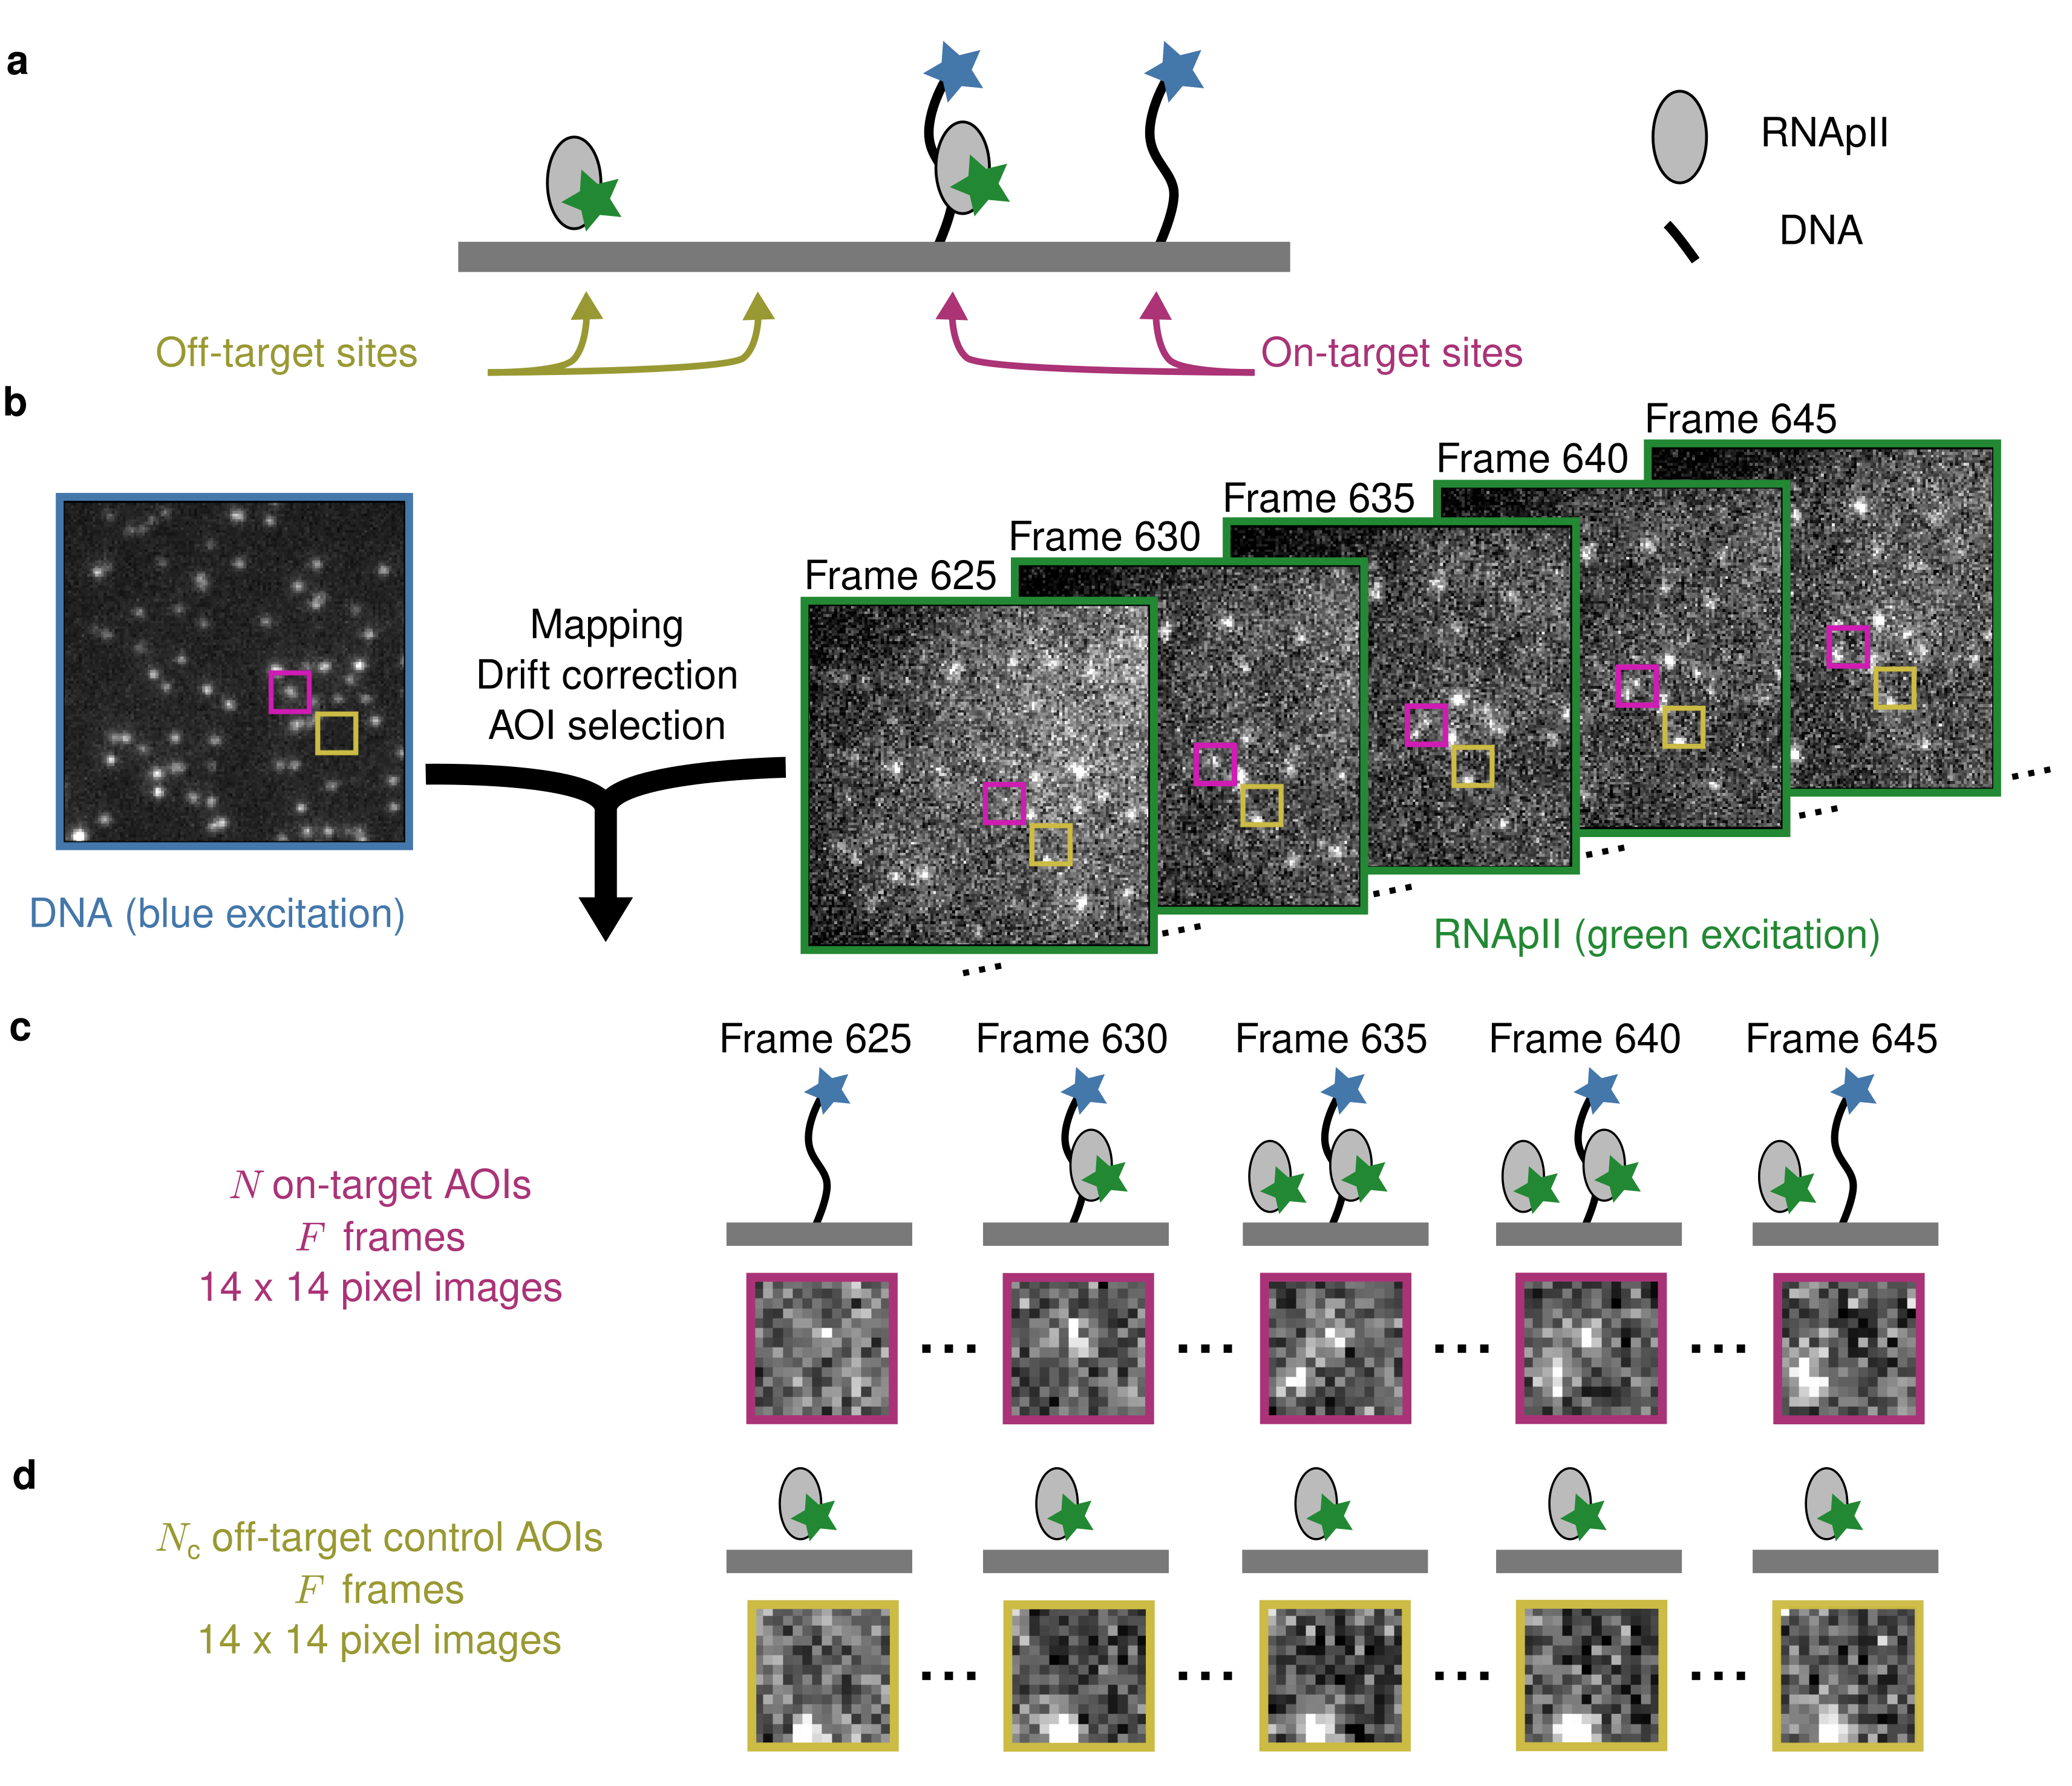
\includegraphics[width=145mm]{figures/figure1/figure1.png}
\caption{\textbf{Example CoSMoS experiment.} \textbf{a}, Experiment schematic. DNA target molecules labeled with a blue-excited fluorescent dye (blue star) are tethered to the microscope slide surface. RNA polymerase II (RNApII) binder molecules labeled with a green-excited dye (green star) are present in solution. \textbf{b}, Data collection and preprocessing. After collecting a single image with blue excitation to identify the location of the DNA molecules, a time sequence of RNApII images were collected with green excitation.  Preprocessing of the images includes mapping of the corresponding points in target and binder channels, drift correction, and identification of two sets of areas of interest (AOIs).  One set corresponds to locations of target molecules (e.g., purple square); the other corresponds to locations where no target is present (e.g., yellow square). \textbf{c}, On-target data. Data are time sequences of $14 \times 14$ pixel AOI images centered at each target molecule. Frames show on-target (e.g., frame 630) and off-target (e.g., frame 645) binding of RNApII molecules. \textbf{d}, Off-target control data. Control data consists of images collected from randomly selected sites at which no target molecule is present. Dataset: Rpb1\textsuperscript{SNAP549} (Extended Data Table 1). }
\label{fig:cosmos_experiment}
\end{figure}

% figure 2
\begin{figure}[h]
\centering
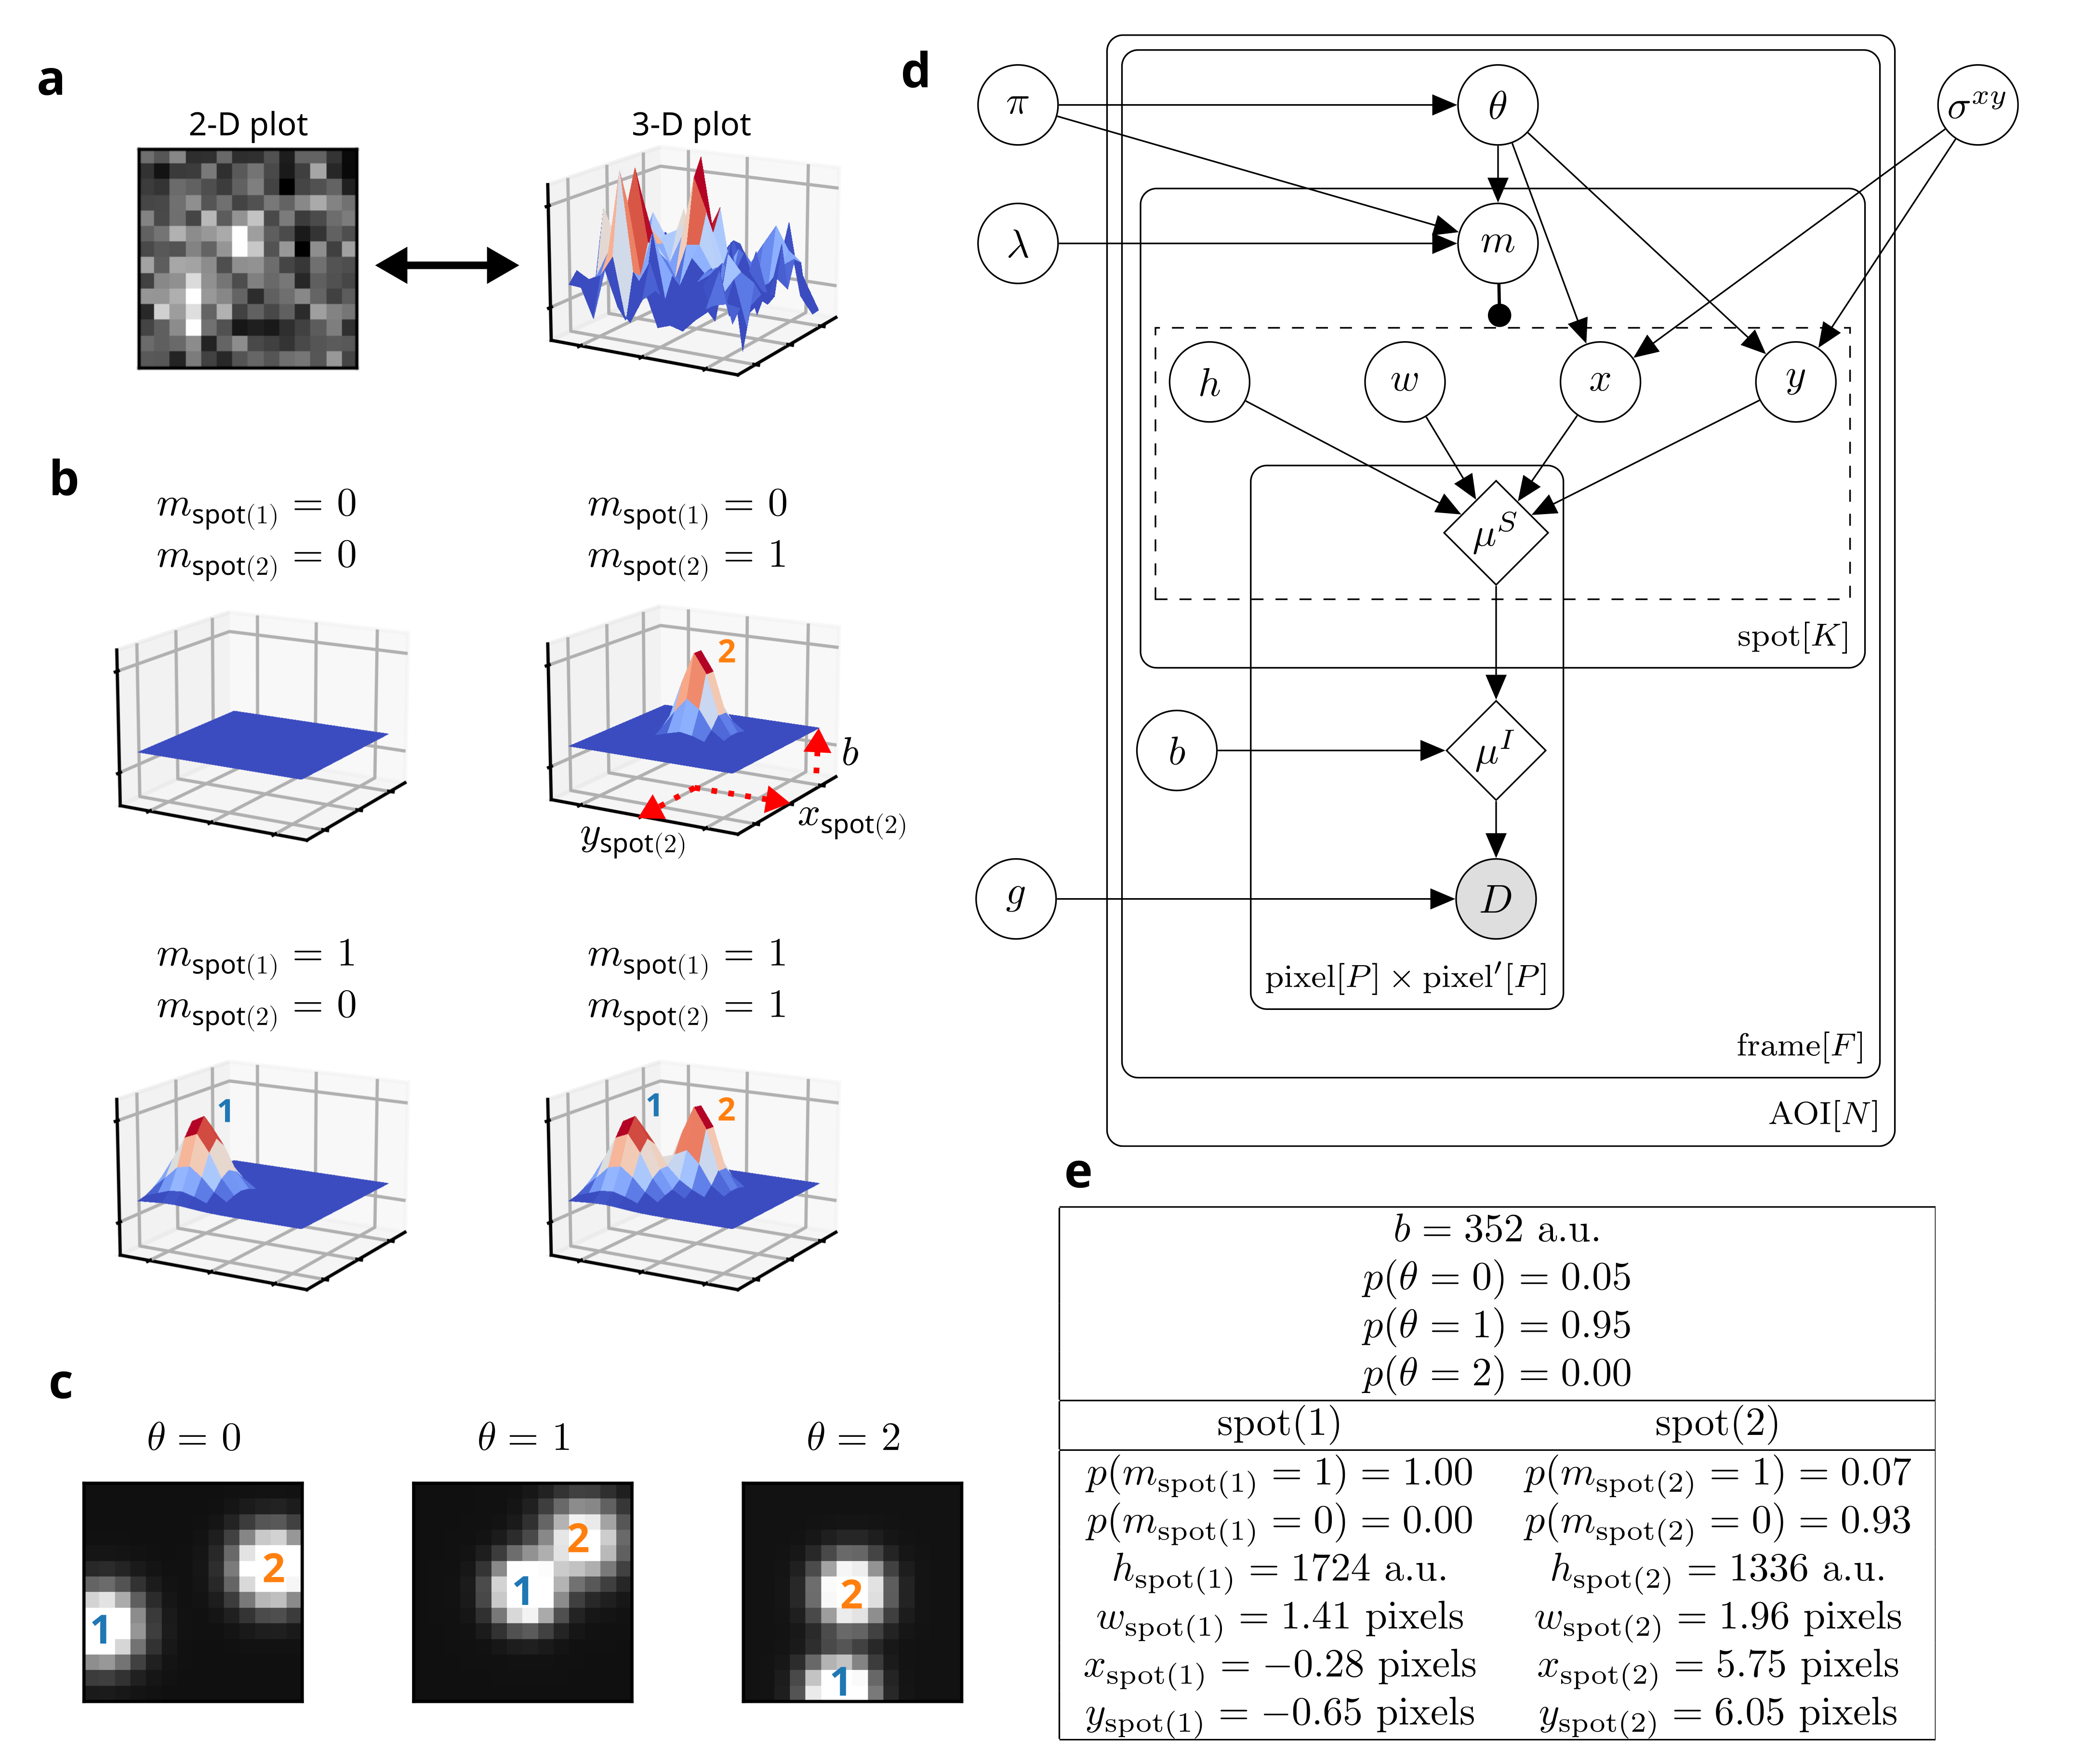
\includegraphics[width=183mm]{figures/figure2/figure2.png}
\label{fig:tapqir_model}
\caption{\textbf{Depiction of the probabilistic image model and model parameters.} \textbf{a}, Example AOI image from an observed dataset ($D$). The image is a matrix (AOI) of $14 \times 14$ pixel intensities which is shown here as both a 2-D grayscale image and as a 3-D intensity plot. The image contains two spots, one is centered at target location (image center) and the other is located off-target. \textbf{b}, Examples of four idealized noise-free image representations ($\mu^I$). Image representations consist of zero, one, or two idealized spots ($\mu^S$) superimposed on a constant background ($b$). Each fluorescent spot is represented as a 2-D Gaussian parameterized by integrated intensity ($h$), width ($w$), and position ($x$, $y$). We assume that each image contains a maximum of one specifically bound fluorescent molecule. The presence of spots is encoded in the binary spot existence indicator $m$. \textbf{c}, Simulated idealized images illustrating different values of the target-specific spot index parameter $\theta$. $\theta = 0$ corresponds to a case when no specifically bound molecule is present; $\theta = 1$ or 2 corresponds to the cases in which the specifically bound molecule is spot 1 or 2, respectively. \textbf{d}, Condensed graphical representation of the probabilistic generative model. Model parameters are depicted as circles and deterministic functions as diamonds. Observed image ($D$) is represented by a shaded circle. Related nodes are connected by edges, with an arrow pointing towards the dependent node (e.g., the shape of each 2-D Gaussian spot $\mu^S$ depends on spot parameters $h$, $w$, $x$, and $y$). The dashed box represents activation of spot parameters based on the spot existence indicator $m$. Plates (rounded rectangles) contain entities that are repeated for the number of instances displayed at the bottom-right corner: number of AOIs ($N$), frame count ($F$), and/or maximum number of spots in a single image ($K=2$). A more complete version of the graphical model specifying the relevant probability distributions is given in Extended Data Fig. 1a. \textbf{e}, Table of mean parameter values inferred from applying model (\textbf{d}) to the full dataset containing the image in (\textbf{a}). Image models in (\textbf{b}) correspond to parameters shown. }
\end{figure}

% figure 3
\begin{figure}[h]
\centering
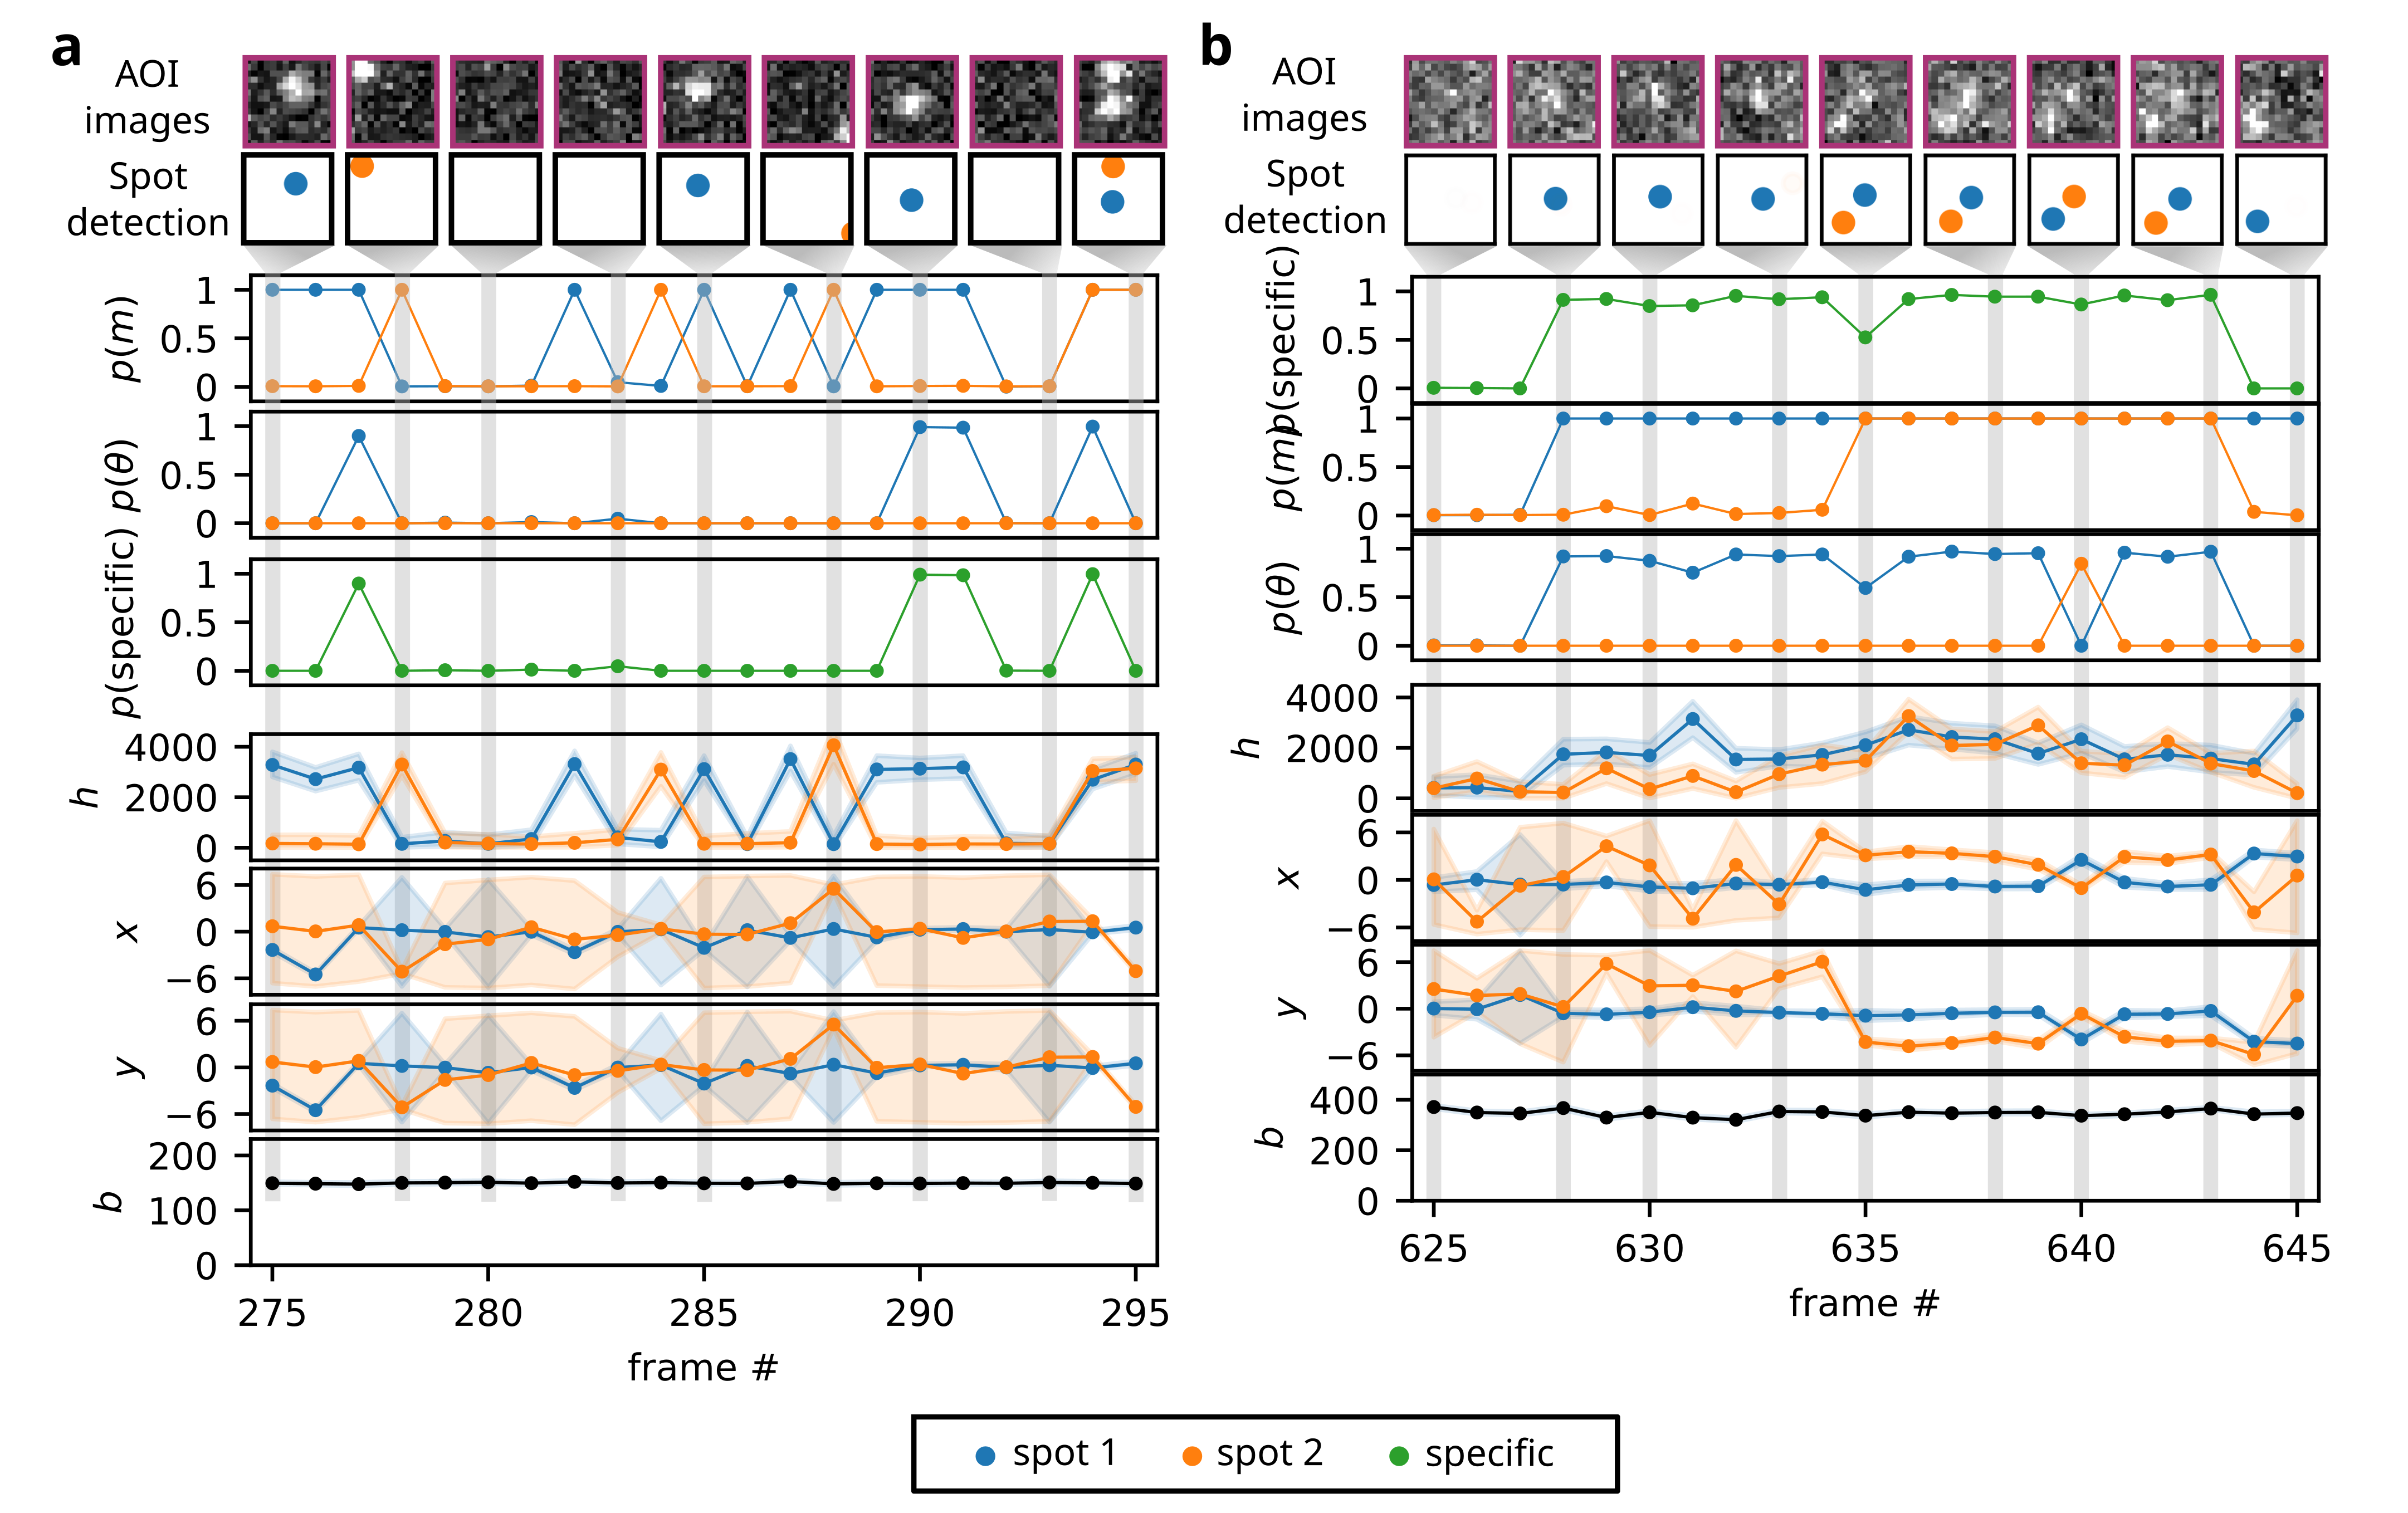
\includegraphics[width=\textwidth]{figures/figure3/figure3.png}
\caption{\textbf{Tapqir analysis and inferred model parameters.} \textbf{a},\textbf{b}, Tapqir was applied to simulated data (\textbf{a}) (height3000 in Supplementary Data 1) and experimental data (\textbf{b}) (Rpb1\textsuperscript{SNAP549} in Extended Data Table 1). Each panel shows a short extract from a single target location in the dataset. AOI images and corresponding schematics of Tapqir detected spots (color transparency corresponds to spot presence probability) are shown for the subset of frames indicated by gray shaded stripes in the plots. Top three plots show the probability of spot $k$ being present $p(m_{\mathsf{spot}(k)}=1)$, the probability of spot $k$ being target-specific $p(\theta=k)$, and the probability of there being any target-specific spot in a frame $p(\mathsf{specific}) = p(\theta>0)$.  Bottom four graphs show mean values (points) with estimated uncertainties (shading, $95\%$ CI) for the inferred integrated spot intensity $h$, spot position $x$ and $y$, and background intensity $b$. }
\label{fig:tapqir_analysis}
\end{figure}

% figure 4
\begin{figure}[h]
\centering
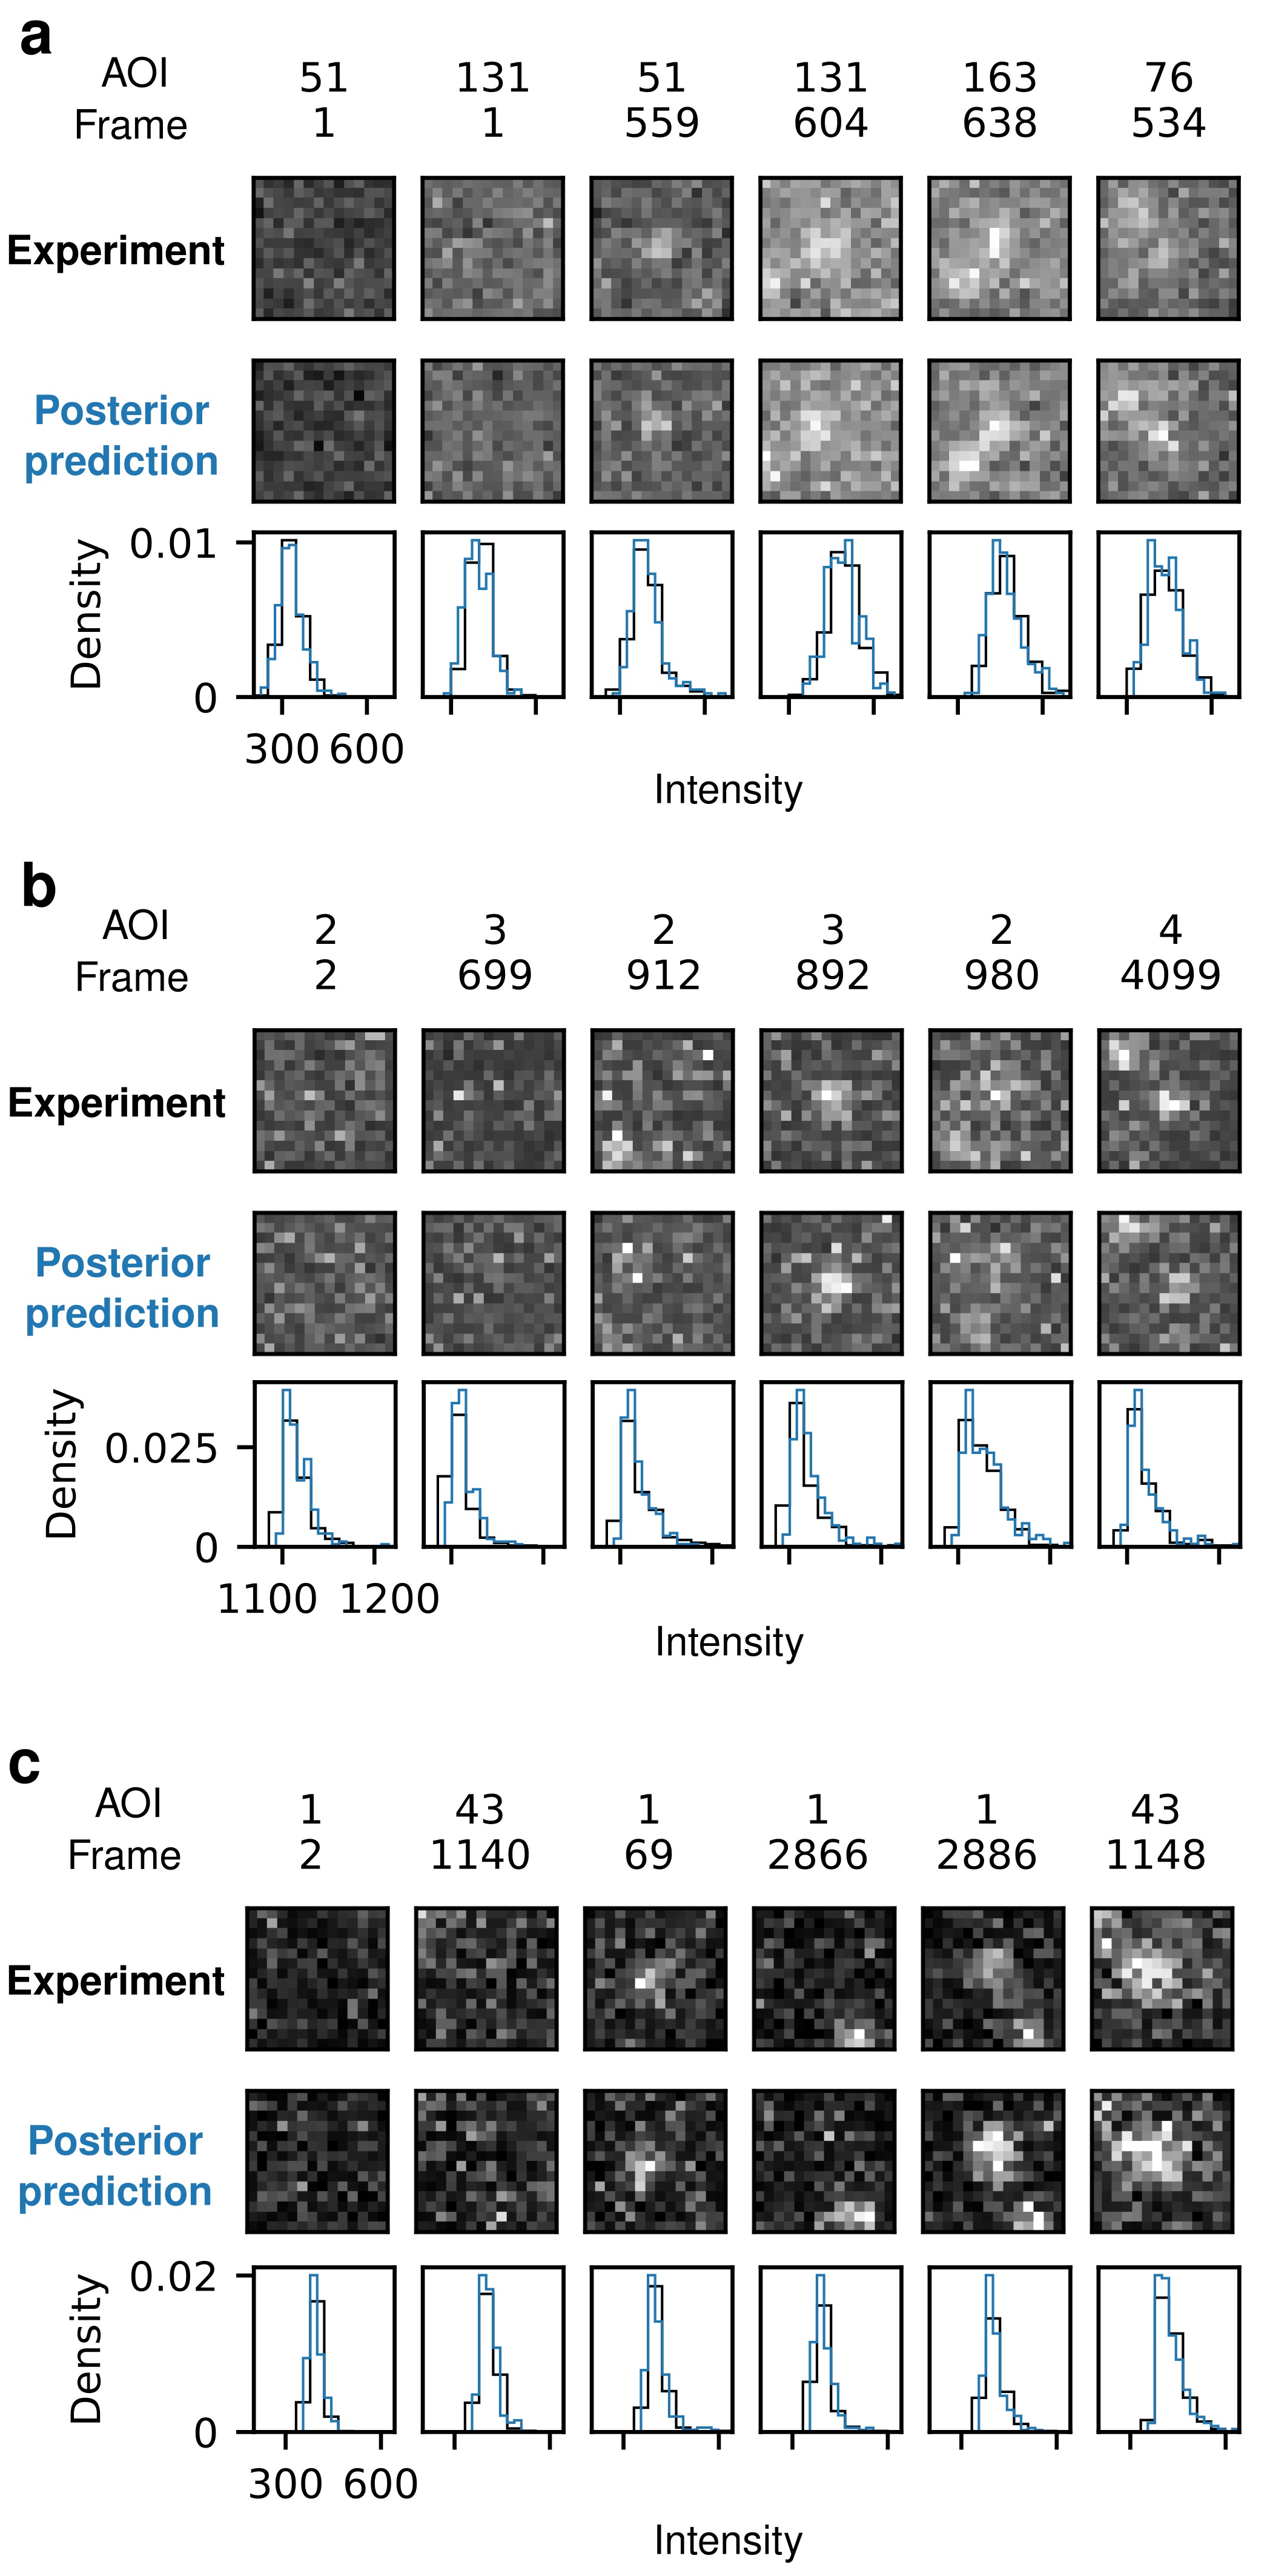
\includegraphics[width=89mm]{figures/figure4/figure4.png}
\caption{\textbf{Reproduction of experimental data by posterior predictive sampling.} Example frames are shown from datasets Rpb1\textsuperscript{SNAP549}-DNA\textsuperscript{488} (\textbf{a}: $\mathrm{SNR}=1.61$), $\sigma^{54}$RNAPCy3-597P255 (\textbf{b}: $\mathrm{SNR}=3.93$), and $\sigma^{54}$RNAPCy3-598P2993 (\textbf{c}: $\mathrm{SNR}=4.18$) in Extended Data Table 1. In each panel top row shows images of the experimental data and middle row shows images sampled from the posterior distributions. Bottom row shows intensity distributions of experimental data and posterior predictions of images shown. }
\label{fig:posterior_samples}
\end{figure}

% figure 5
\begin{figure}[h]
\centering
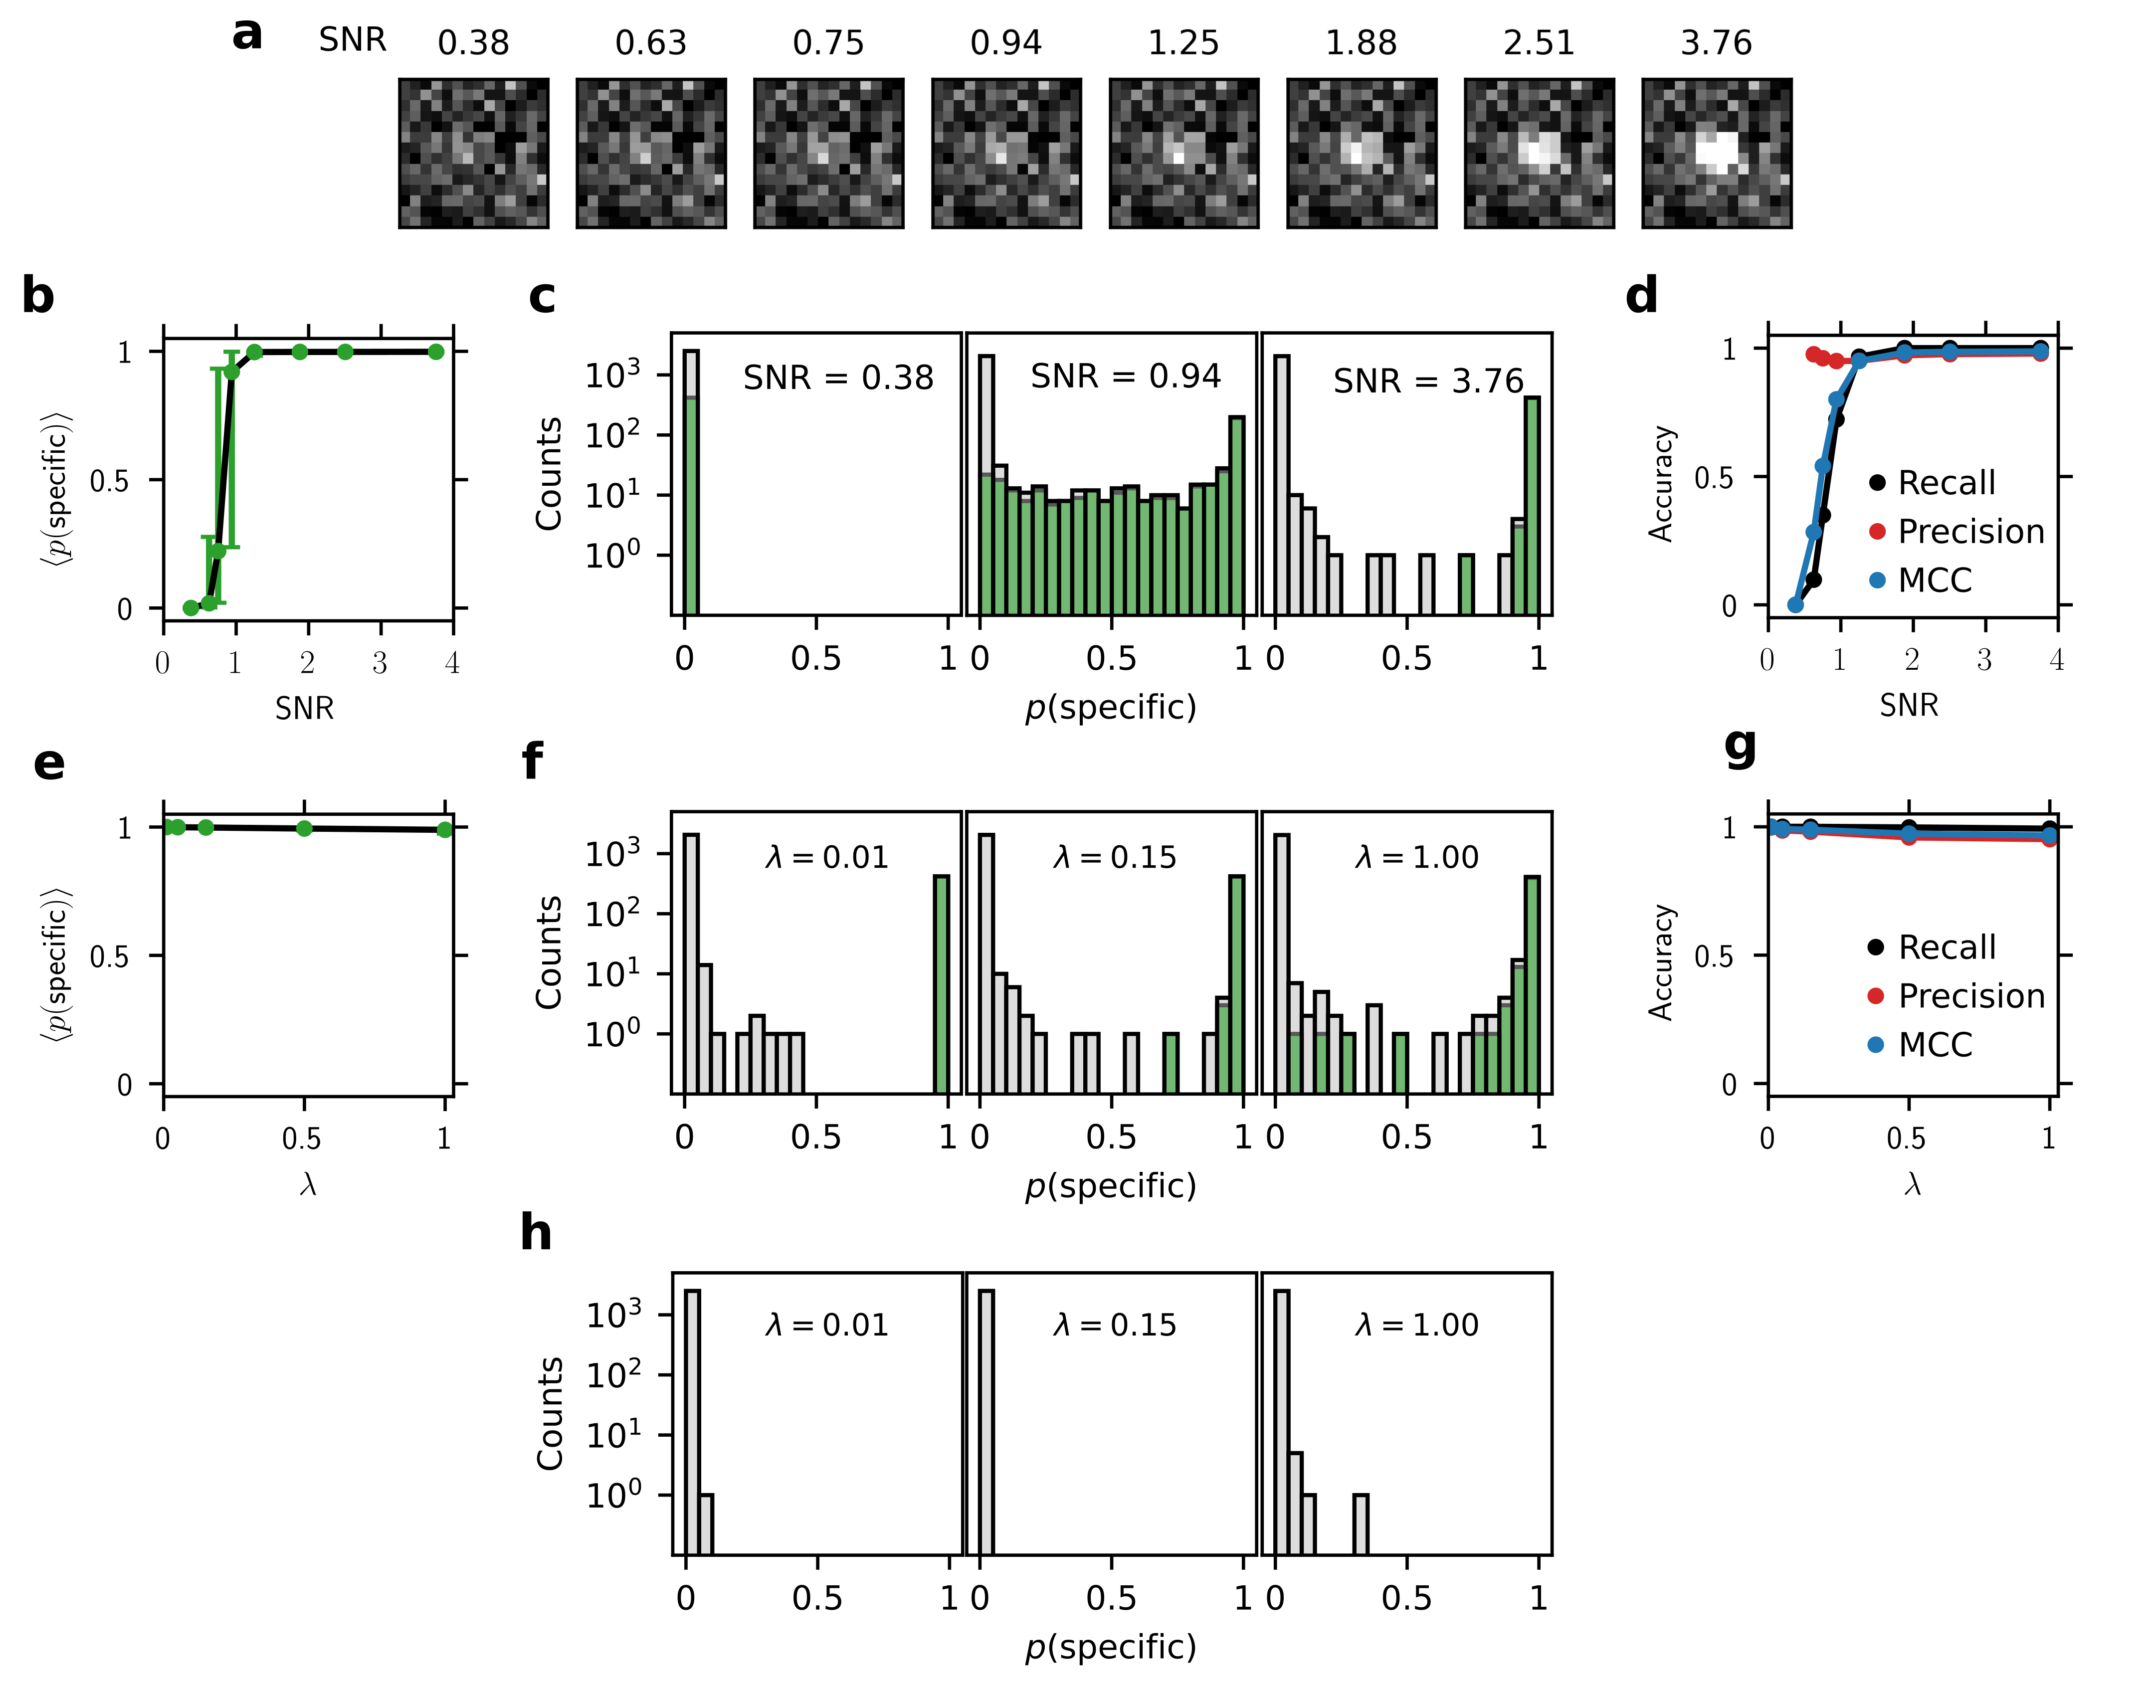
\includegraphics[width=1\textwidth]{figures/figure5/figure5.png}
\caption{\textbf{Tapqir performance on simulated data with different SNRs or different non-specific binding rates.} \textbf{a-d}, Analysis of the simulated data over a range of SNR where SNR was varied by changing spot intensity  $h$ while keeping other parameters constant (Supplementary Data 1). \textbf{a}, Example images showing the appearance of the same target-specific spot simulated with increasing SNR.   \textbf{b}, Mean of Tapqir-calculated target-specific spot probability $p(\mathsf{specific})$ (with 68\% C.I.) for the subset of images where target-specific spots  are known to be present. \textbf{c}, Histograms of $p(\mathsf{specific})$ for selected simulations with SNR indicated. Data are shown as stacked bars for images known to have (green, 15\%) or not have (gray, 85\%) target-specific spots.  Count is zero for bins where bars are not shown. \textbf{d}, Accuracy of Tapqir image classification with respect to presence/absence of a target-specific spot. Accuracy was assessed by MCC, recall, and precision (see Text and Methods). \textbf{e-g}, Same as in (\textbf{b-d}) but for the data simulated over a range of non-specific binding rates $\lambda$ at fixed SNR = 3.76 (Supplementary Data 3). \textbf{h}, Same as in (\textbf{c}) but for the data simulated over a range of non-specific binding rates $\lambda$ with no target-specific binding ($\pi = 0$) (Supplementary Data 4).}
\label{fig:tapqir_performance}
\end{figure}

% figure 6
\begin{figure}[h]
\centering
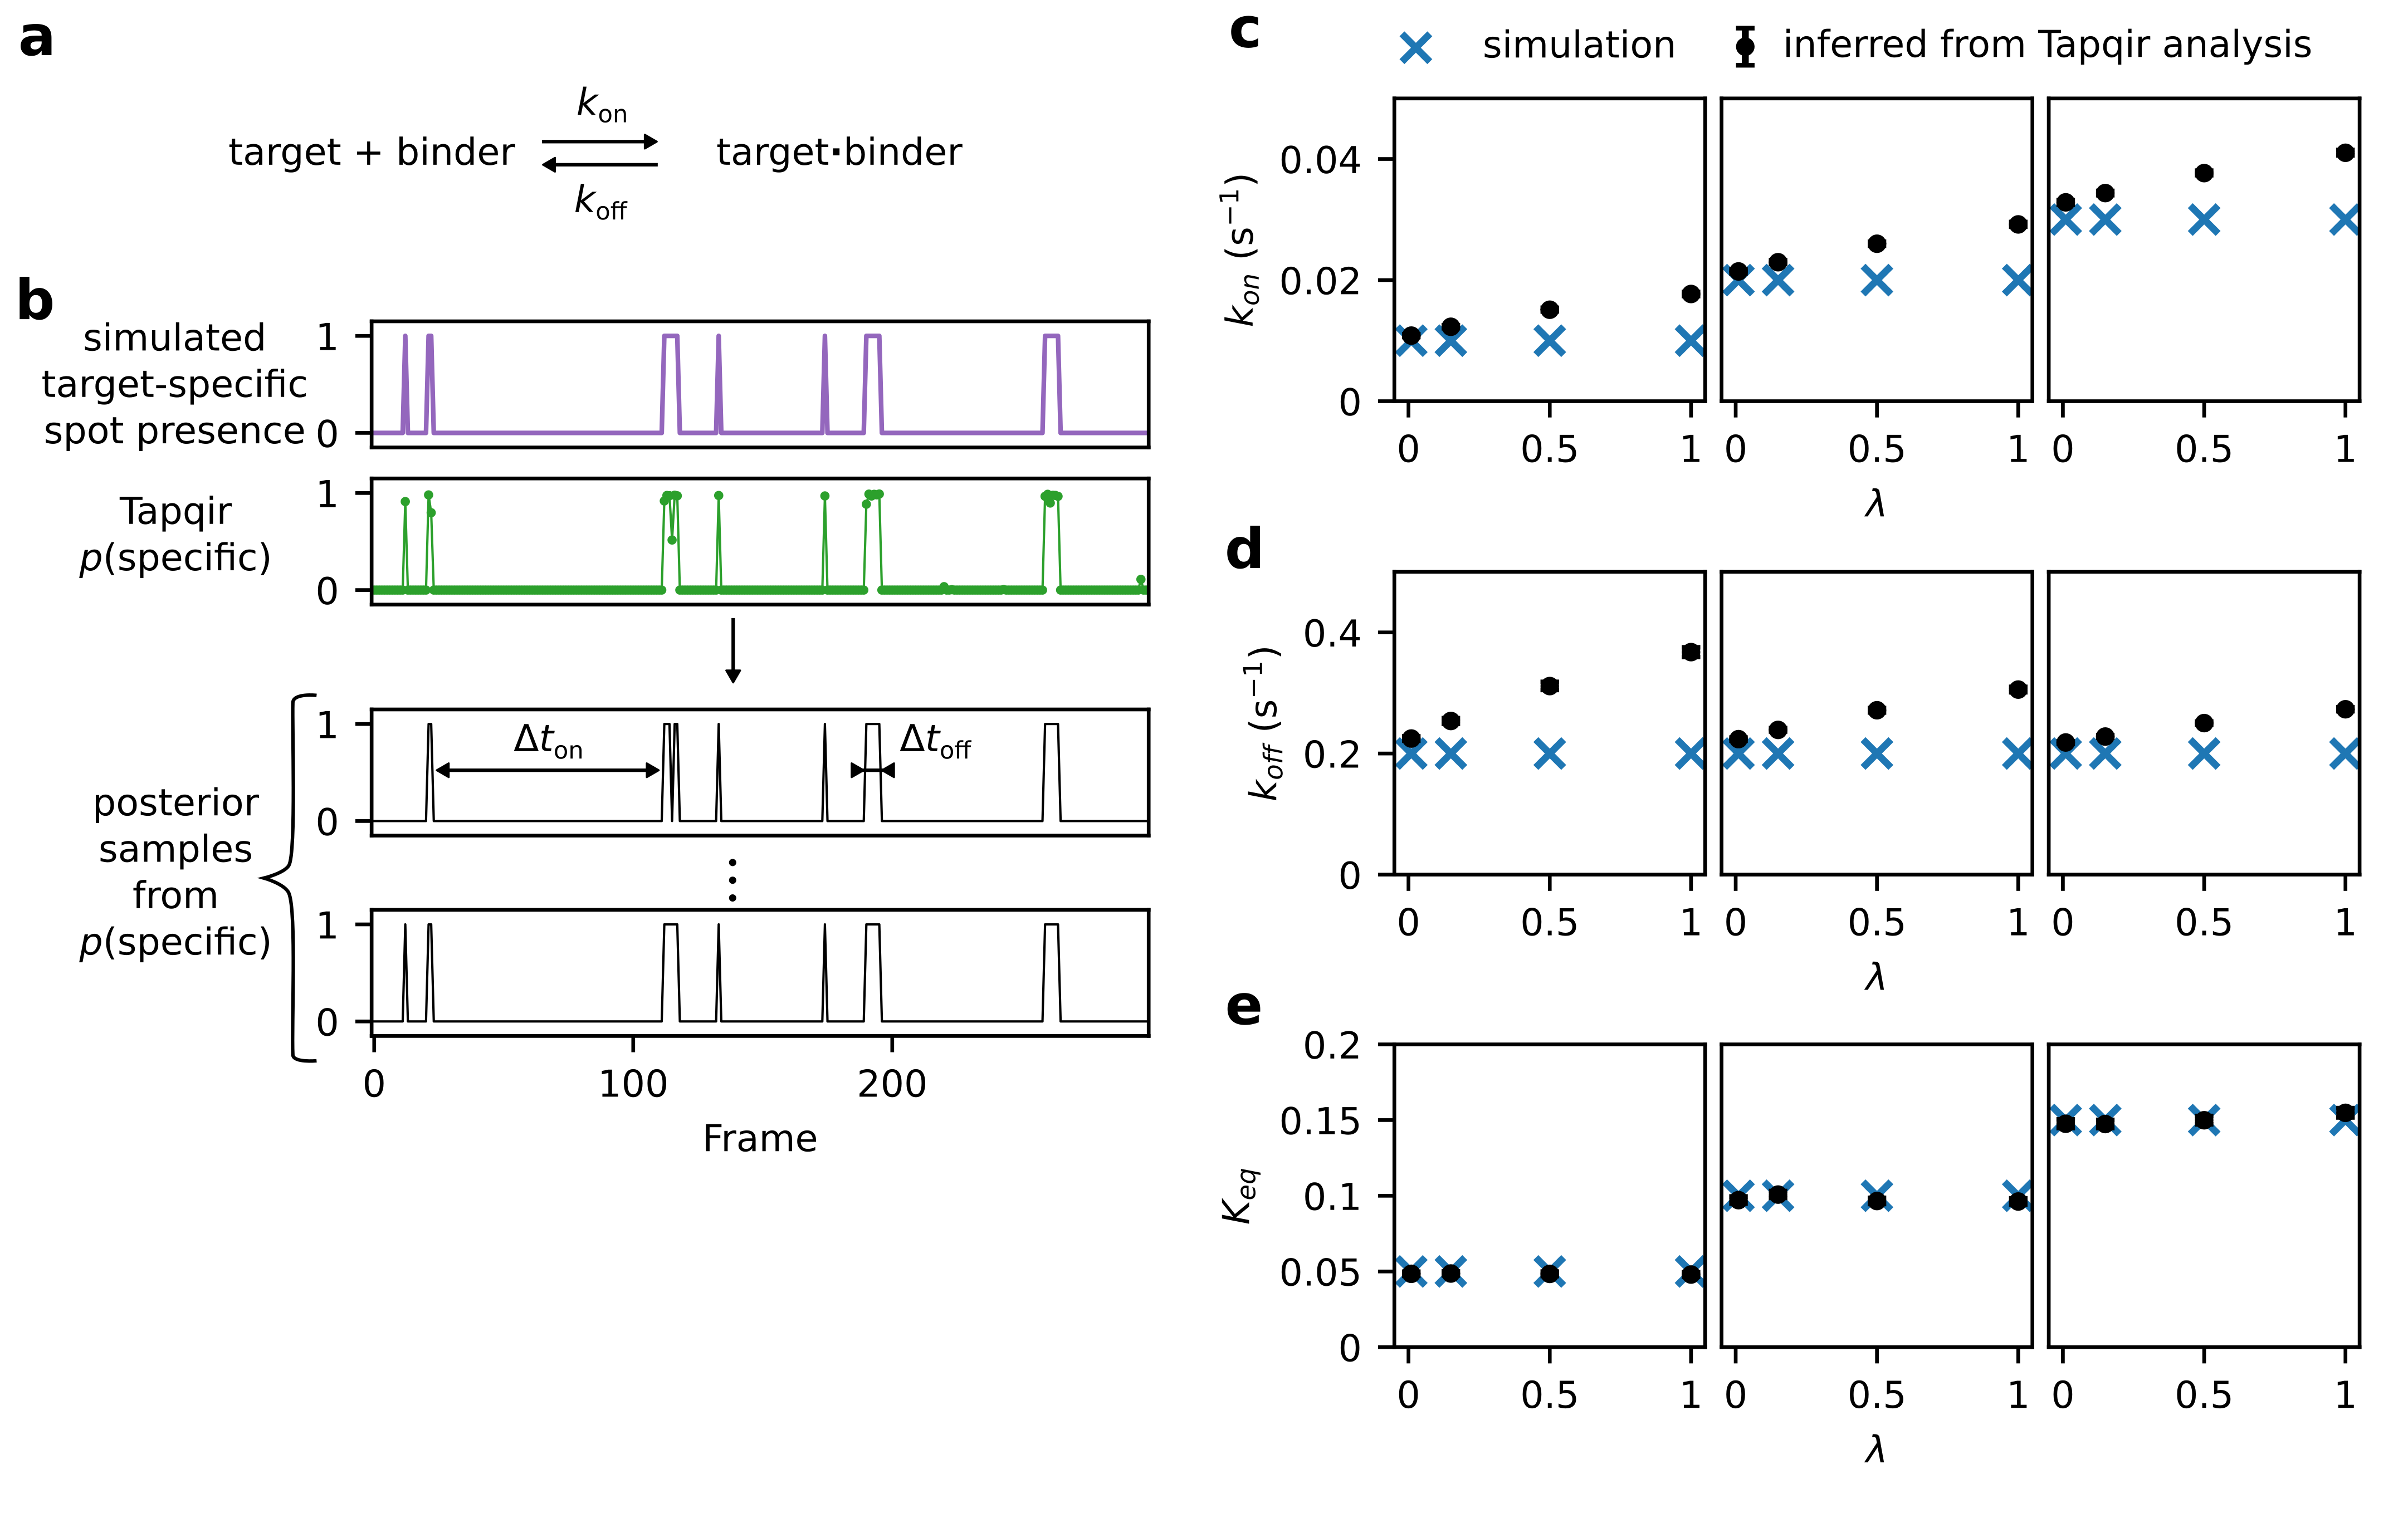
\includegraphics[width=89mm]{figures/figure6/figure6.png}
\caption{\textbf{Tapqir analysis of association/dissociation kinetics and thermodynamics.} \textbf{a} Chemical reaction scheme for a one-step association/dissociation reaction at equilibrium with apparent first-order binding and dissociation rate constants $k_{\mathrm{on}}$ and $k_{\mathrm{off}}$, respectively. \textbf{b}, Simulation of the reaction in (\textbf{a}) and scheme for analysis with Tapqir. Simulation used $\mathrm{SNR} = 3.76$, $k_\mathrm{on} = 0.02$ s$^{-1}$, $k_\mathrm{off} = 0.2$ s$^{-1}$, and a high target-nonspecific binding frequency $\lambda = 1$ (Supplementary Data X, dataset kon0.02lambda1). Full datasets consisted of 100 AOI locations and 1000 frames for both on-target and control data. Shown is a short extract of data from a single target location in the simulation.  Plots show simulated presence/absence of the target-specific spot  (purple) and Tapqir-calculated estimate of corresponding target-specific spot probability $p(\mathsf{specific})$ (green). One thousand binary traces (black) were sampled from the $p(\mathsf{specific})$ posterior distribution and used to compute binding-present ($\Delta t_\mathrm{on}$) and binding-absent ($\Delta t_\mathrm{off}$) dwell times. \textbf{c,d,e}, Kinetic and equilibrium constants from a set of simulations using a range of $k_\mathrm{on}$ values and  target-nonspecific spot frequencies $\lambda$, with constant $k_\mathrm{off} = 0.2$ s$^{-1}$. \textbf{c} Values of $k_{\mathrm{on}}$ used in simulation (blue) and inferred from the distribution of $\Delta t_\mathrm{off}$ (black). \textbf{d}, Same as (\textbf{c}) but for $k_{\mathrm{off}}$ used in simulation and inferred from $\Delta t_\mathrm{on}$. \textbf{e},  Same as (\textbf{c}) but for dissociation equilibrium constant $K_{\mathrm{eq}} = k_{\mathrm{on}} / k_{\mathrm{off}}$ used in simulation and inferred from $\pi$ as $K_{\mathrm{eq}} = \pi / (1 - \pi)$. }
\label{fig:kinetic_analysis}
\end{figure}

% figure 7
\begin{figure}[h]
\centering
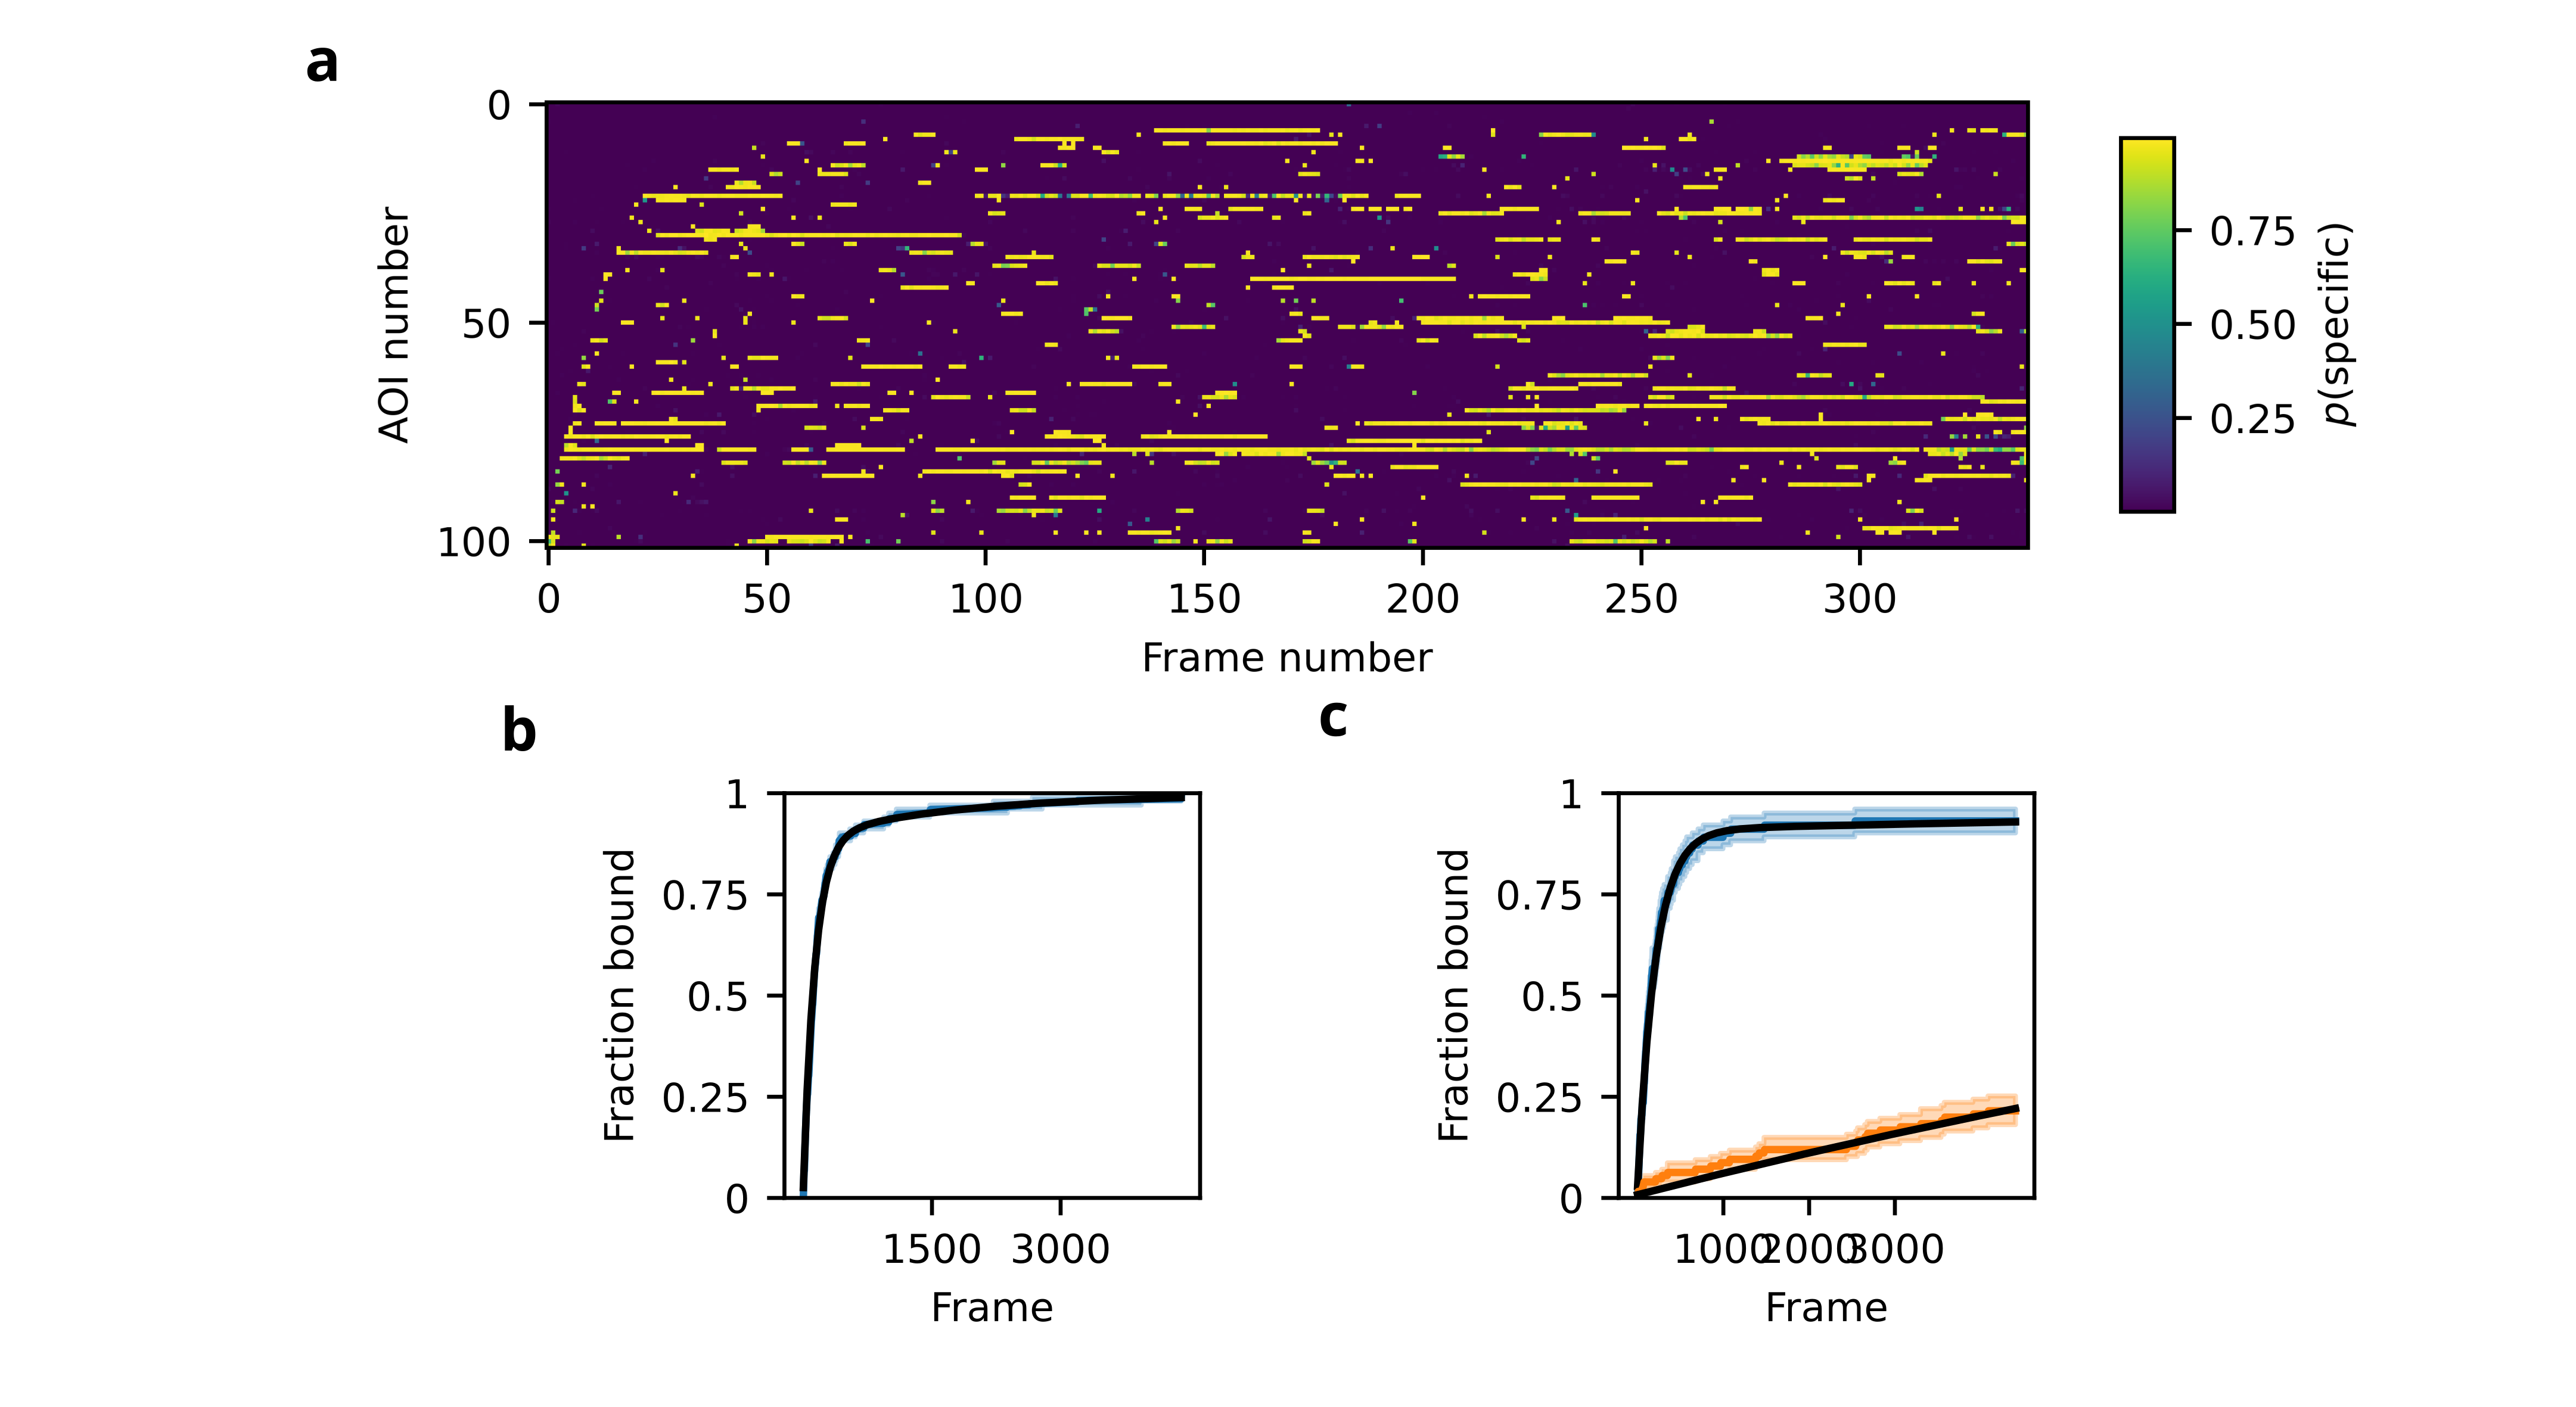
\includegraphics[width=\textwidth]{figures/figure7/figure7.png}
\caption{\textbf{Kinetic analysis of experimental data.}   \textbf{a}, Rastergram representation of Tapqir-calculated target-specific spot  probabilities $p(\mathsf{specific})$ (color scale) for every 13\textsuperscript{th} frame of data at 102 different target locations.  AOIs were ordered by decreasing times-to-first-binding. Data set: $\sigma^{54}$RNAPCy3-597P255 in Extended Data Table 1. \textbf{b,c}, Determining the association rate constant for the same data set by  time-to-first-binding analysis using Tapqir (\textbf{b}: $k_\mathrm{a} = (6.74\pm0.43) \times 10^{-3}$ s$^{-1}$, $k_\mathrm{ns} = (5.8\pm1.7) \times 10^{-4}$ s$^{-1}$) and an empirical spot-picker method (\textbf{c}: $k_\mathrm{a} = (4.8\pm0.6) \times 10^{-3}$ s$^{-1}$, $k_\mathrm{ns} = (5.4\pm1.0) \times 10^{-5}$ s$^{-1}$) (ref).   Cumulative fraction of target sites that exhibited one or more binding events by the indicated time (blue) and fit curve (black) yielding best-fit values for $k_\mathrm{a}$, $k_\mathrm{ns}$, and $A_\mathrm{f}$. Shading indicates 68\% confidence interval. Fitting protocol is different for the two methods; the spot-picker method fits both the target sites and off-target control data (orange) whereas Tapqir incorporates the control data in its $p(\mathsf{specific})$ calculation.
}
\label{fig:experimental_data}
\end{figure}

\clearpage
\newpage
\section*{Extended Data}
\pagebreak

\renewcommand{\figurename}{Extended Data Fig.}
\renewcommand{\tablename}{Extended Data Table}
% \renewcommand{\thetable}{S\arabic{table}}
\setcounter{figure}{0}

\begin{figure}[t]
\centering
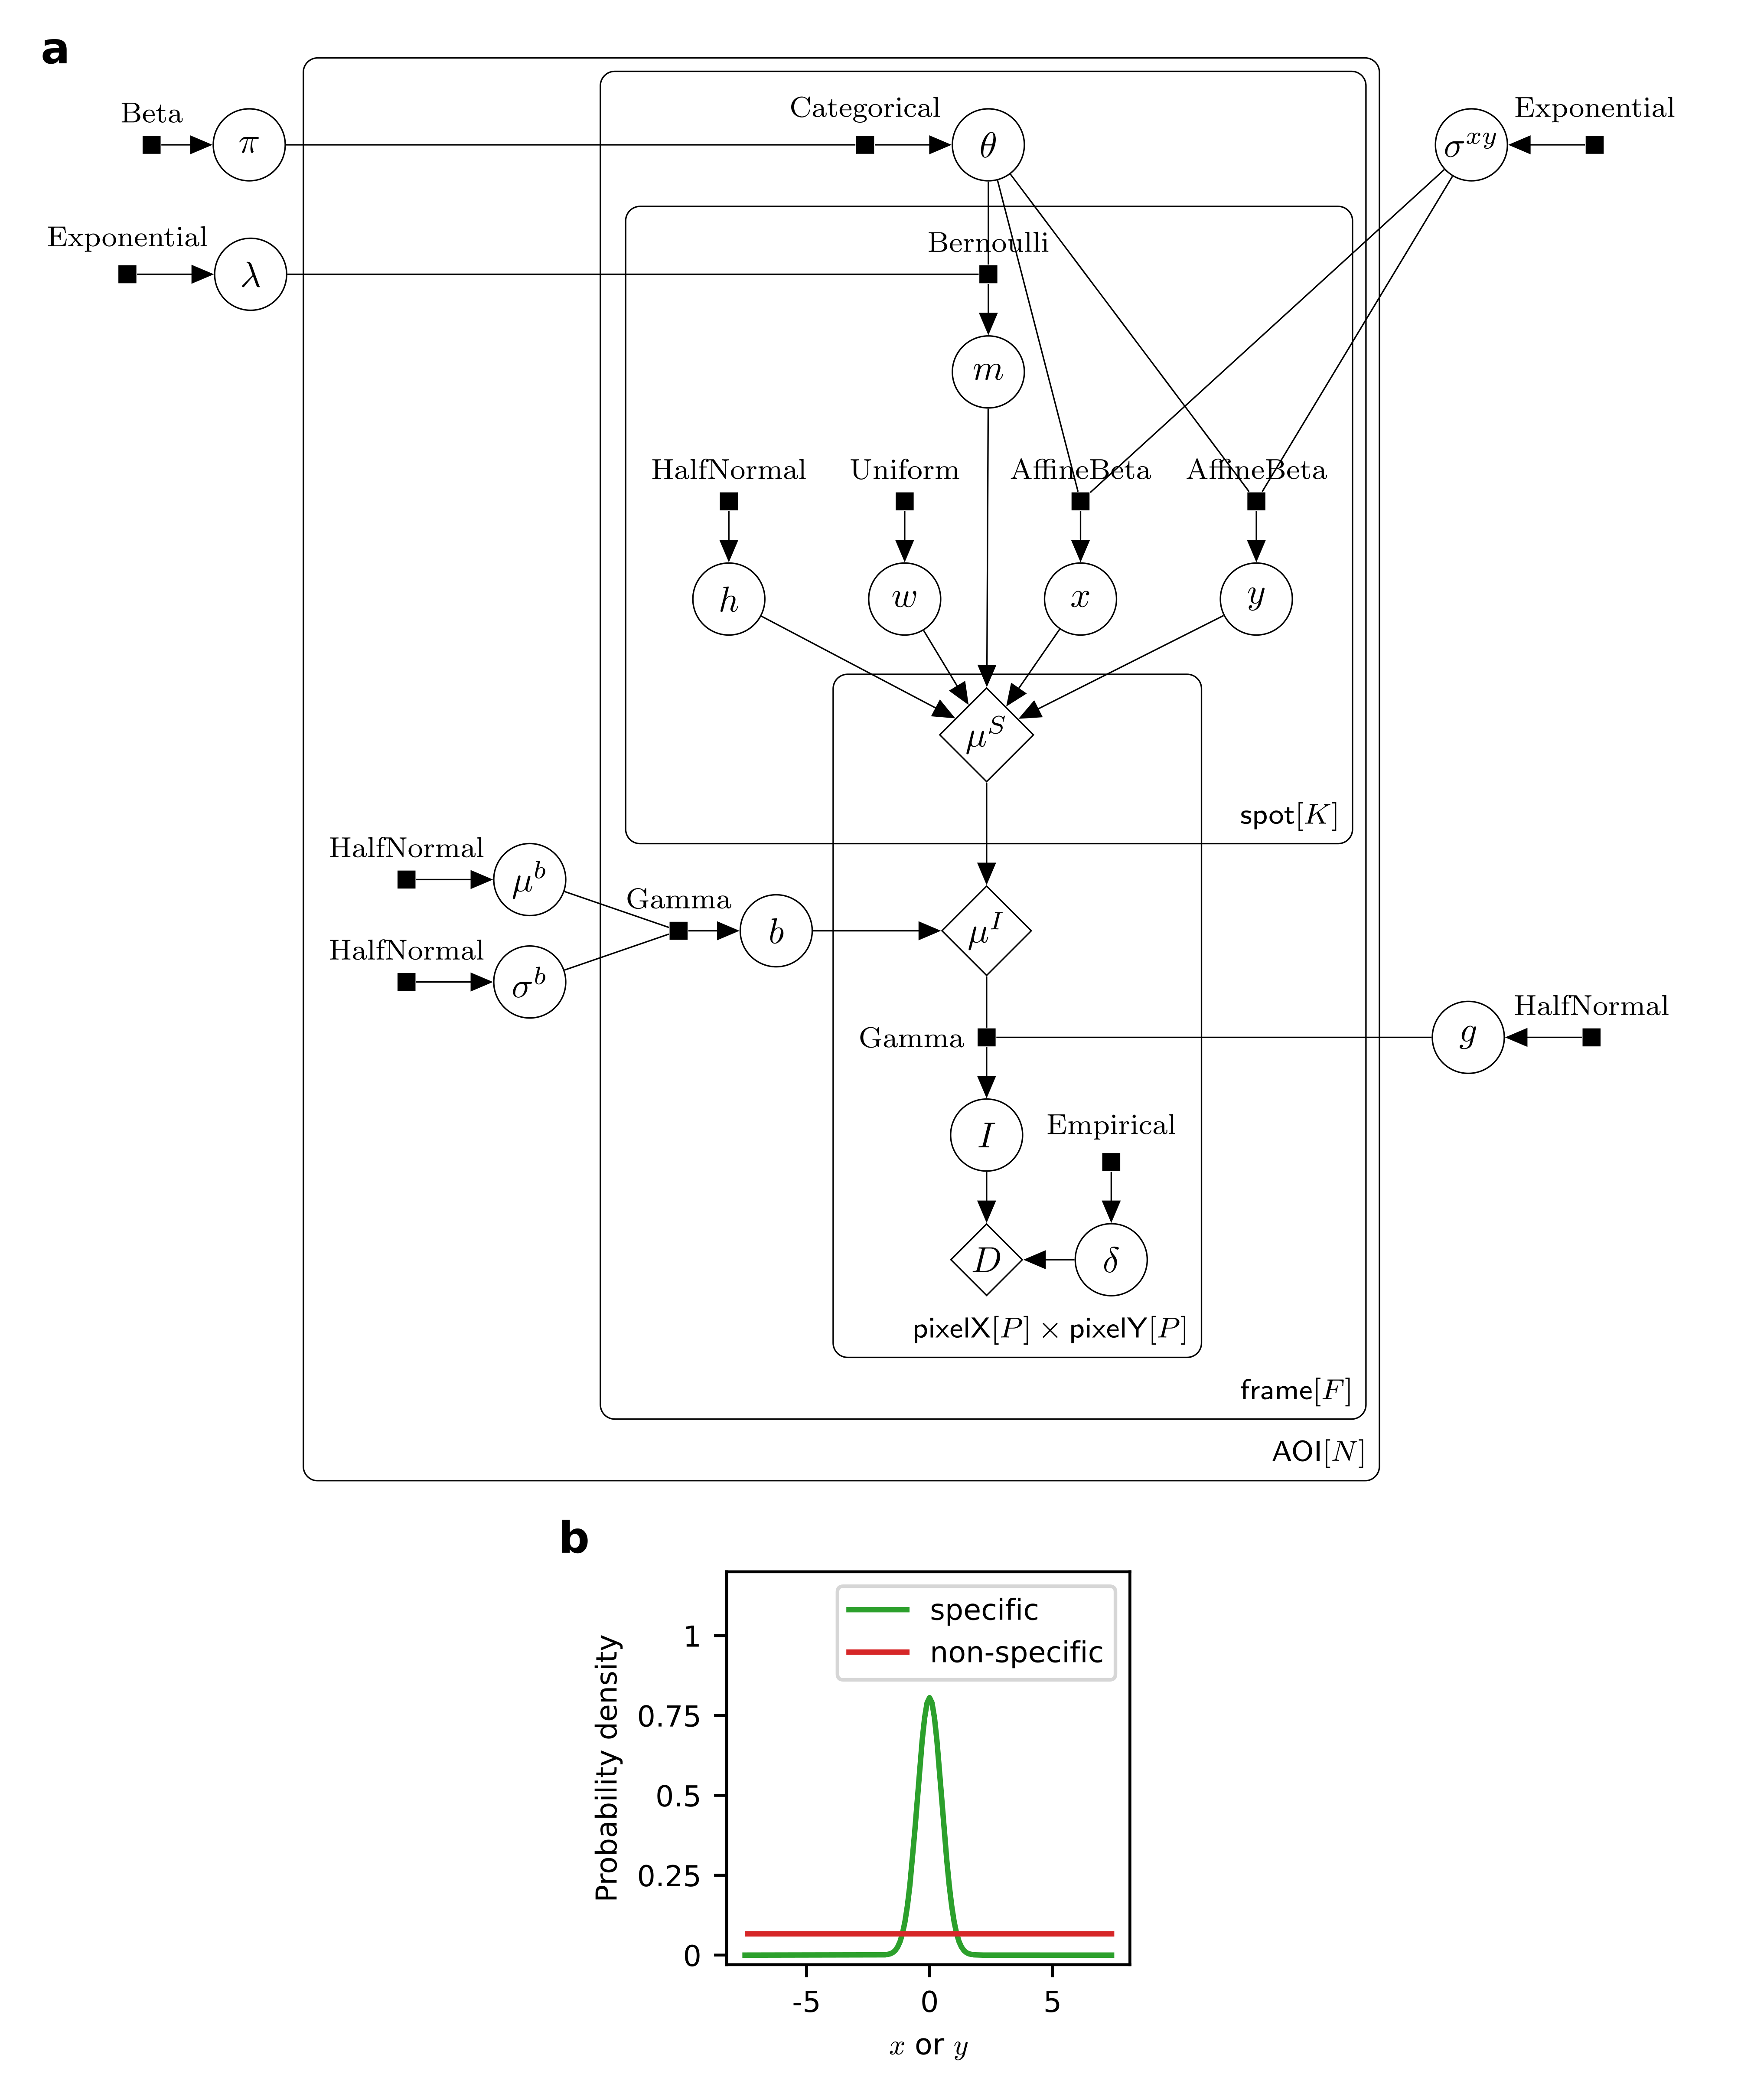
\includegraphics[width=183mm]{extended-data/figure1/figure1.png}
\label{fig:full_model}
\end{figure}

%\addtocounter{figure}{-1}
\begin{figure} [t]
\caption{\textbf{Extended graphical representation of the generative probabilistic model and the prior distributions for $x$ and $y$ spot position parameters.} \textbf{a}, Directed factor graph representation (ref) of model parameters and parameter distributions. Model parameters are depicted as circles, parameter distributions as small filled squares, and deterministic functions as diamonds. Names of the probability distributions are written next to the squares. Input parameters and output parameters are connected by lines, with an arrow pointing towards the dependent parameter. Observed image ($D$) is the sum of the noisy photon-dependent image ($I$) and the photon-independent camera offset ($\delta$). The dashed box represents selection of spot parameters based on the spot existence indicator $m$. Plates (rounded rectangles) contain nodes that are repeated for the number of instances displayed at the bottom-right corner: number of AOIs ($N$), frame count ($F$), maximum number of spots in a single image ($K=2$), and number of image pixels ($P \times P$). \textbf{b}, Prior distributions of $x$ and $y$ for specific and non-specific binding. Probability densities for $x$ and $y$ are defined in the range of the image $-(P+1)/2$, $(P+1)/2$ and are conditional on the identity of the spot (specific or non-specific).  Probability densities for $x$ and $y$ parameters are identical. }
\end{figure}
have a row above each data set with an experiment description, align columns
\clearpage

\begin{figure}[h]
\centering
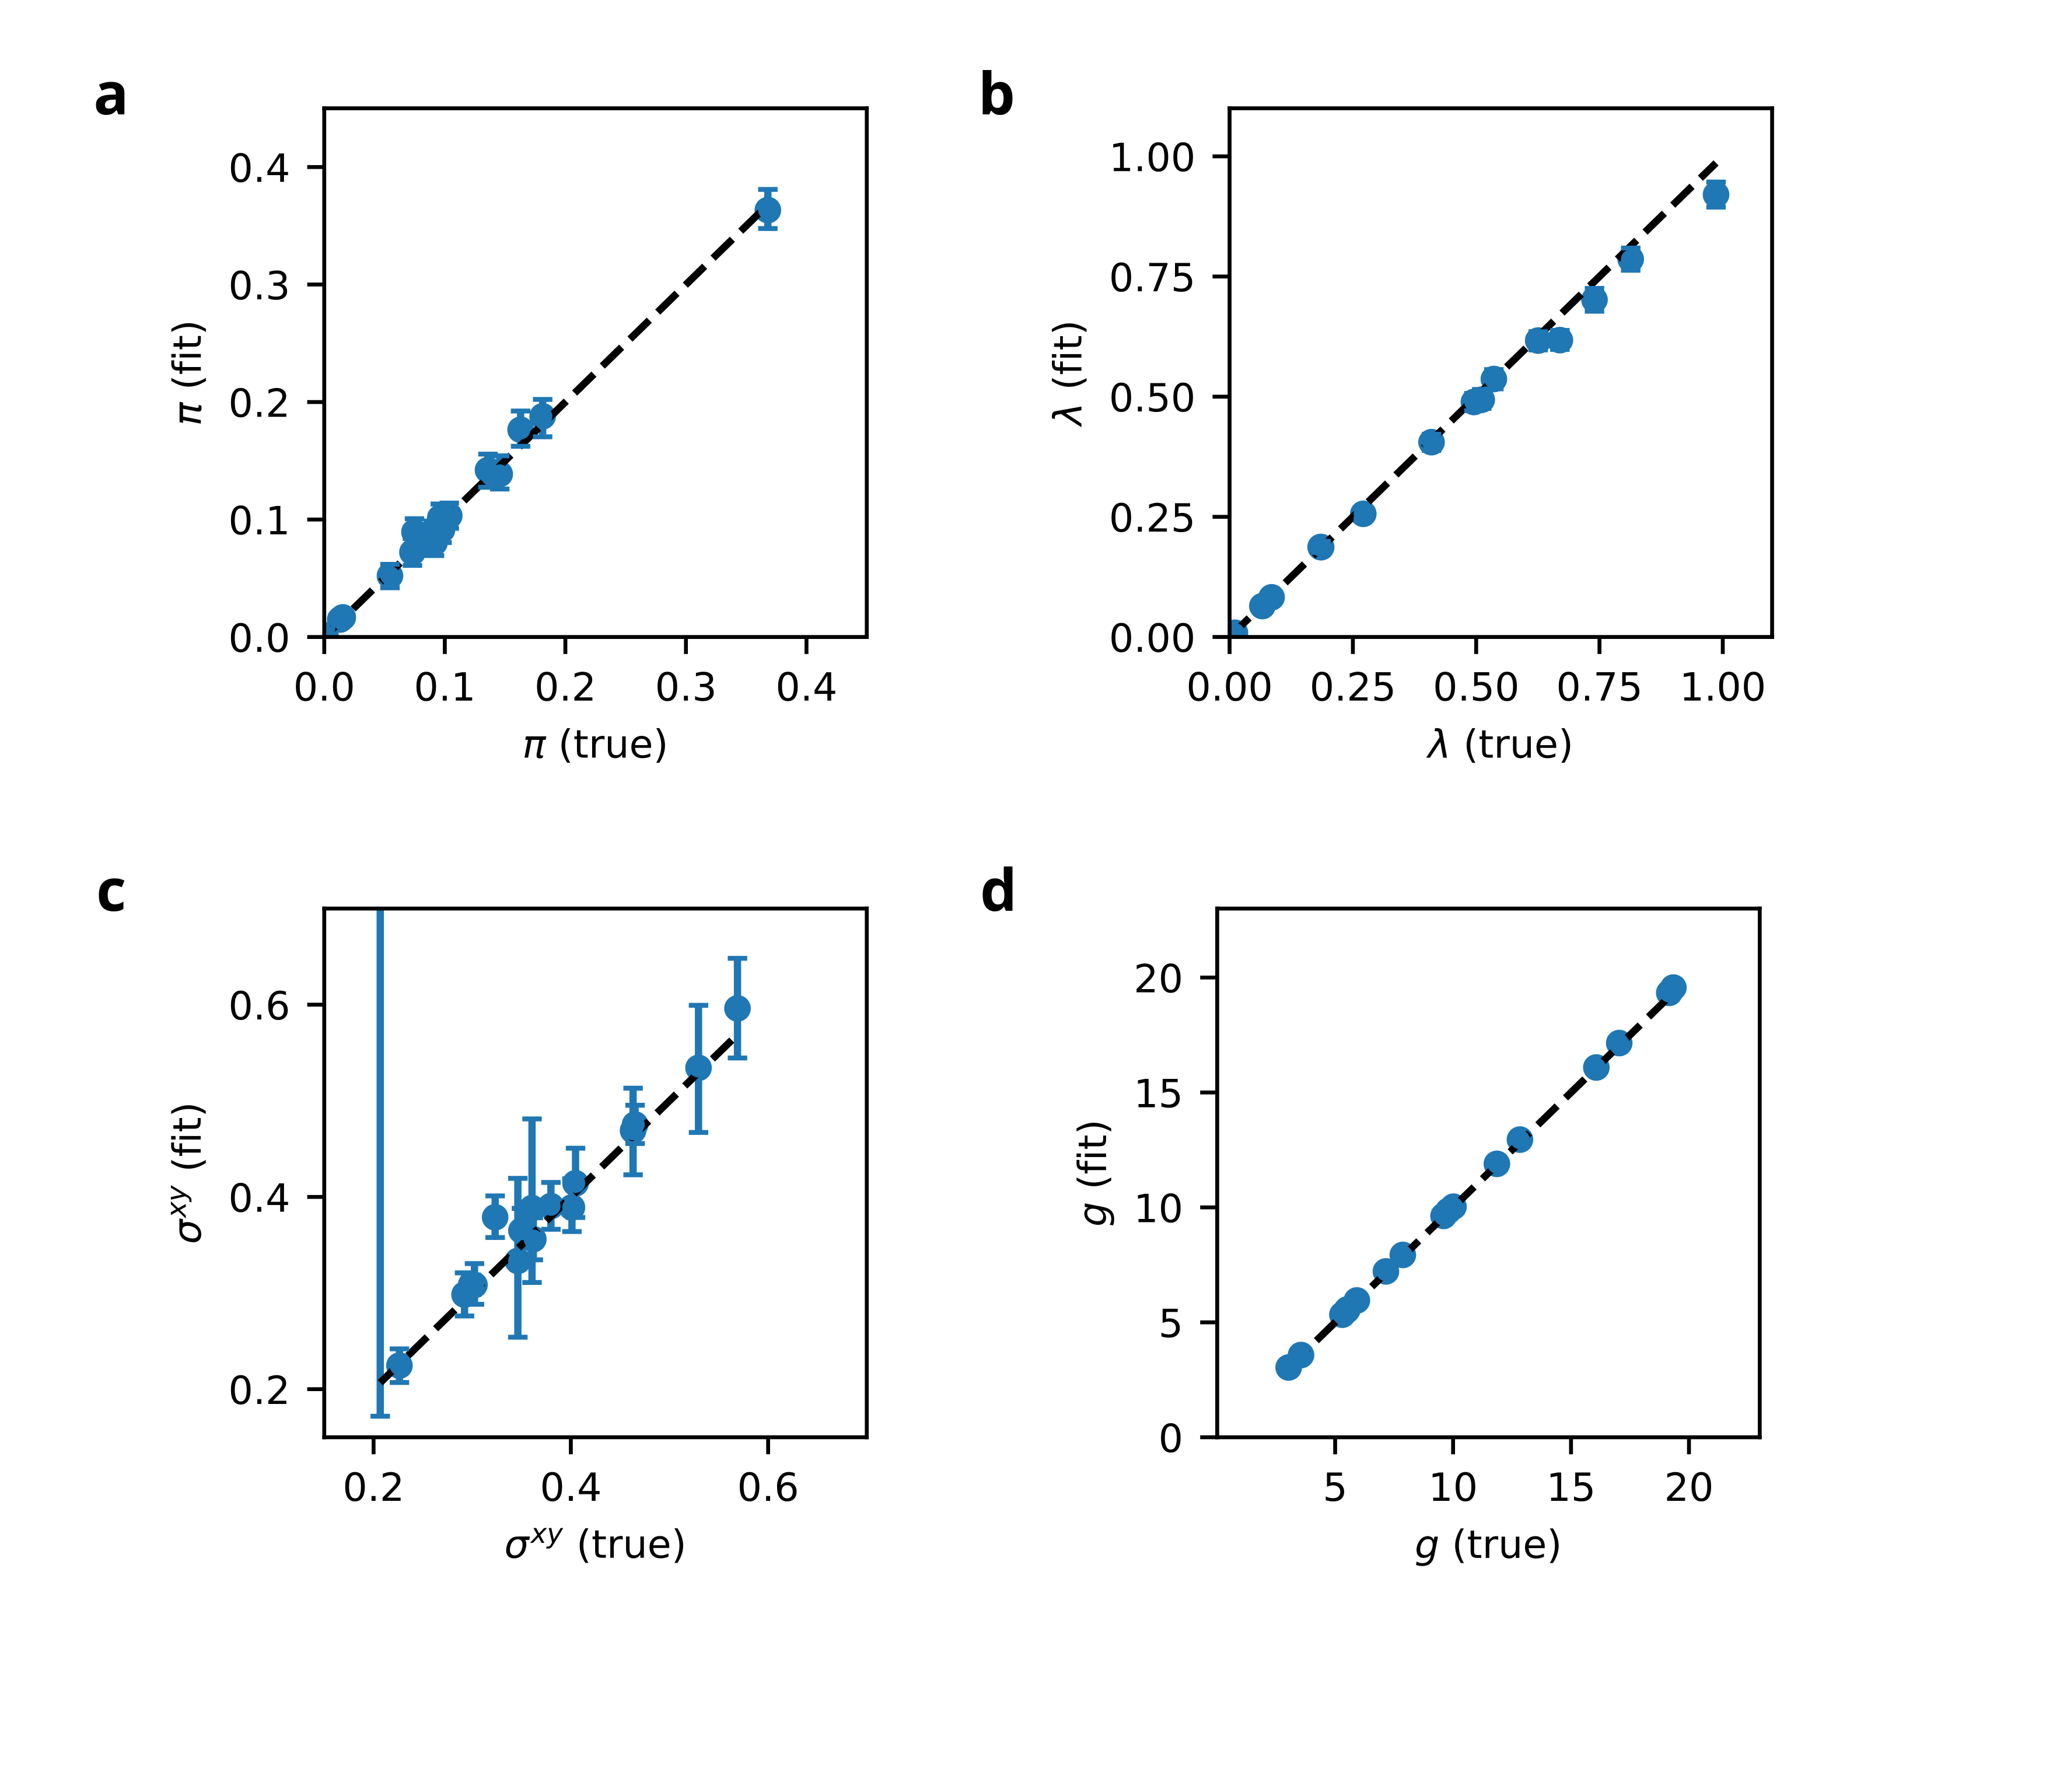
\includegraphics[width=150mm]{extended-data/figure2/figure2.png}
\caption{\textbf{Tapqir analysis of image data simulated using a broad range of global parameters.} Simulations (see Methods) consist of 17 datasets where global parameters ($\pi$, $\lambda$, $\sigma^{xy}$, and $g$) where randomly generated for each dataset (Supplementary Data 2). Simulated data were fit with Tapqir, and parameter values from the fit are plotted against the true parameter values (circles). To guide the eye, dashed lines  indicate identical true and fit values. \textbf{a}, Average specific binding probability $\pi$. \textbf{b}, Nonspecific binding rate $\lambda$. \textbf{c}, Proximity parameter $\sigma^{xy}$. \textbf{d}, Gain of the camera $g$. }
\label{fig:tapqir_global}
\end{figure}
\pagebreak

\begin{figure}[t]
\centering
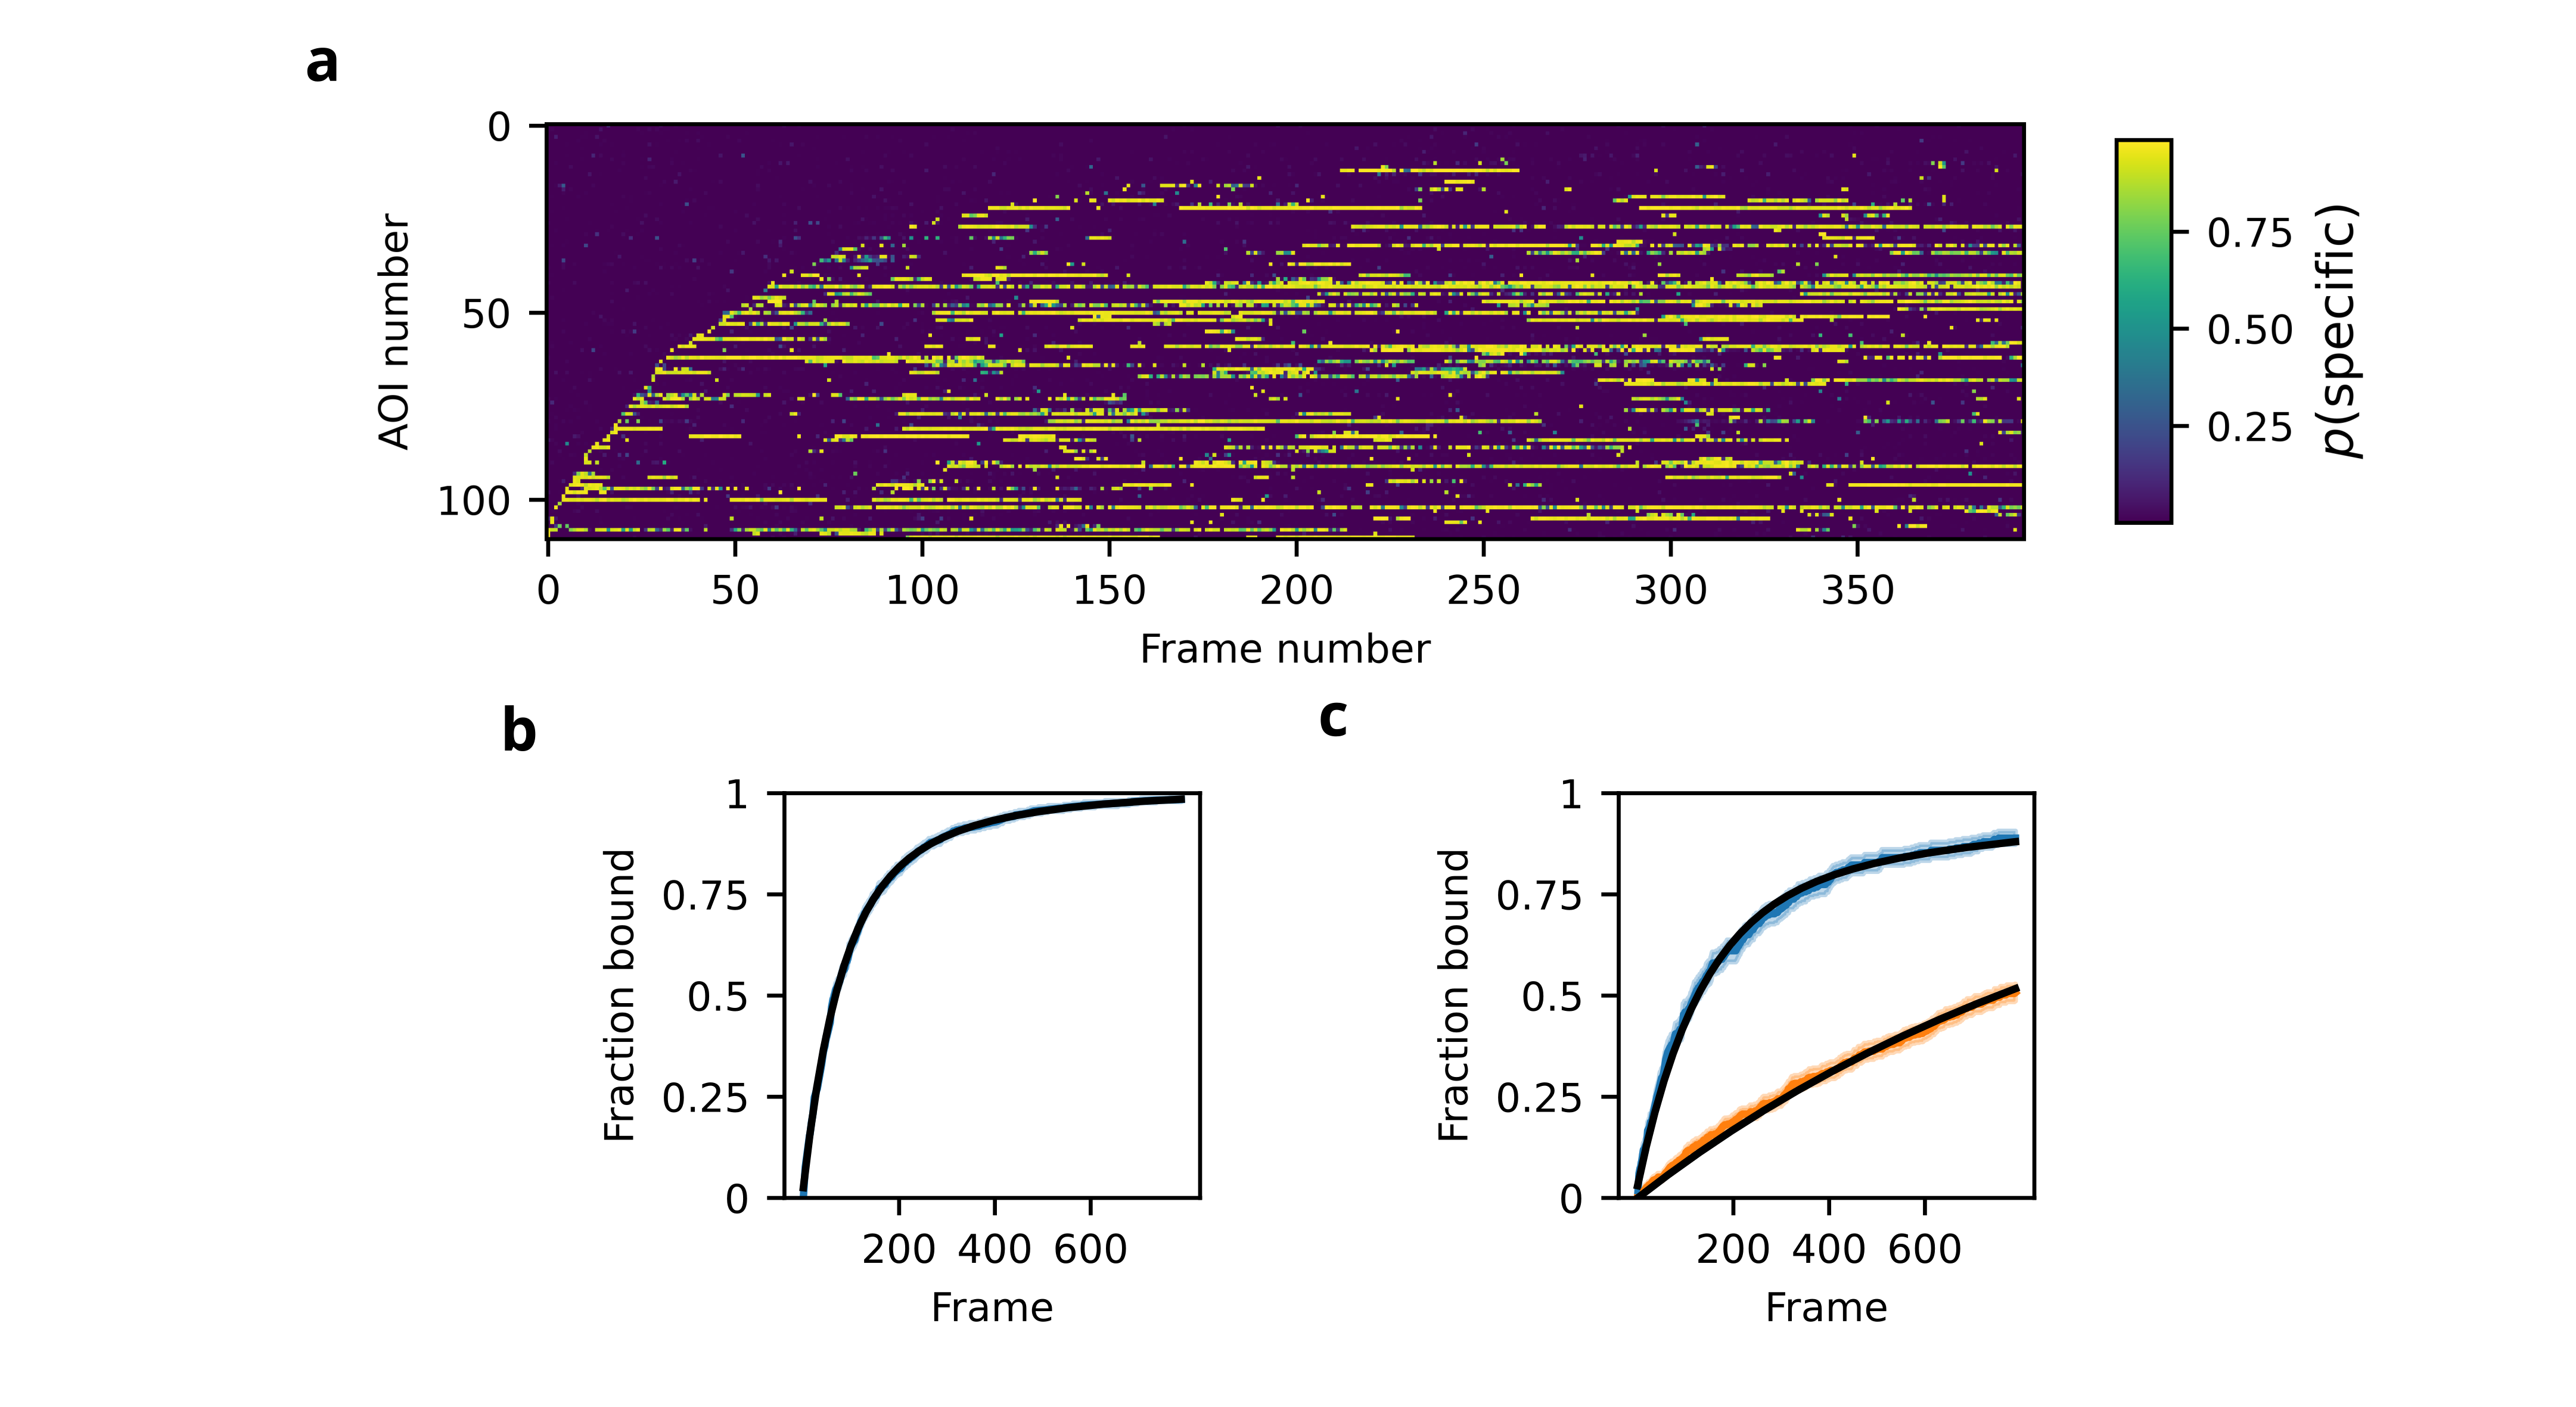
\includegraphics[width=\textwidth]{extended-data/figure3/figure3.png}
\caption{\textbf{Time-to-first binding analysis of experimental data.}  Determining association rates for experimental CoSMoS data using the time-to first binding analysis. \textbf{a}, Rastergram representation of $p(\mathsf{specific})$ (color scale) for every 3\textsuperscript{rd} AOI and every 2\textsuperscript{nd} frame of Rbp1\textsuperscript{SNAP549}-DNA\textsuperscript{488} dataset (Extended Data Table 1). DNA locations ordered by time-to-first binding. \textbf{b,c}, Determining the association rate constant for the same data set by  time-to-first-binding analysis using Tapqir (\textbf{b}: $k_\mathrm{a} = 3.40 \: [2.54, 4.91] \times 10^{-3}$ s$^{-1}$, $k_\mathrm{ns} = 1.34 \: [0.77, 1.86] \times 10^{-3}$ s$^{-1}$, $A_\mathrm{f} = 0.62 \: []$) and an empirical spot-picker method (\textbf{c}: $k_\mathrm{a} = 2.2 \: [1.7, 2.8] \times 10^{-3}$ s$^{-1}$, $k_\mathrm{ns} = 3.1 \: [2.7, 3.5] \times 10^{-4}$ s$^{-1}$, $A_\mathrm{f} = 0.75 \: []$) \cite{Rosen2020-zn}.   Cumulative fraction of target sites that exhibited one or more binding events by the indicated time (blue) and fit curve (black) yielding best-fit values for $k_\mathrm{a}$, $k_\mathrm{ns}$, and $A_\mathrm{f}$. Shading indicates 68\% confidence interval.
}
\label{fig:rpb1snap549}
\end{figure}
\pagebreak
% \textbf{a}, Rastergram representation of Tapqir-calculated target-specific spot  probabilities $p(\mathsf{specific})$ (color scale) for every 13\textsuperscript{th} frame of data at 102 different target locations.  AOIs were ordered by decreasing times-to-first-binding. Data set: $\sigma^{54}$RNAPCy3-597P255 in Extended Data Table 1. \textbf{b,c}, Determining the association rate constant for the same data set by  time-to-first-binding analysis using Tapqir (\textbf{b}: $k_\mathrm{a} = (6.74\pm0.43) \times 10^{-3}$ s$^{-1}$, $k_\mathrm{ns} = (5.8\pm1.7) \times 10^{-4}$ s$^{-1}$) and an empirical spot-picker method (\textbf{c}: $k_\mathrm{a} = (4.8\pm0.6) \times 10^{-3}$ s$^{-1}$, $k_\mathrm{ns} = (5.4\pm1.0) \times 10^{-5}$ s$^{-1}$) (ref).   Cumulative fraction of target sites that exhibited one or more binding events by the indicated time (blue) and fit curve (black) yielding best-fit values for $k_\mathrm{a}$, $k_\mathrm{ns}$, and $A_\mathrm{f}$. Shading indicates 68\% confidence interval. Fitting protocol is different for the two methods; the spot-picker method fits both the target sites and off-target control data (orange) whereas Tapqir incorporates the control data in its $p(\mathsf{specific})$ calculation.
\begin{figure}[t]
\centering
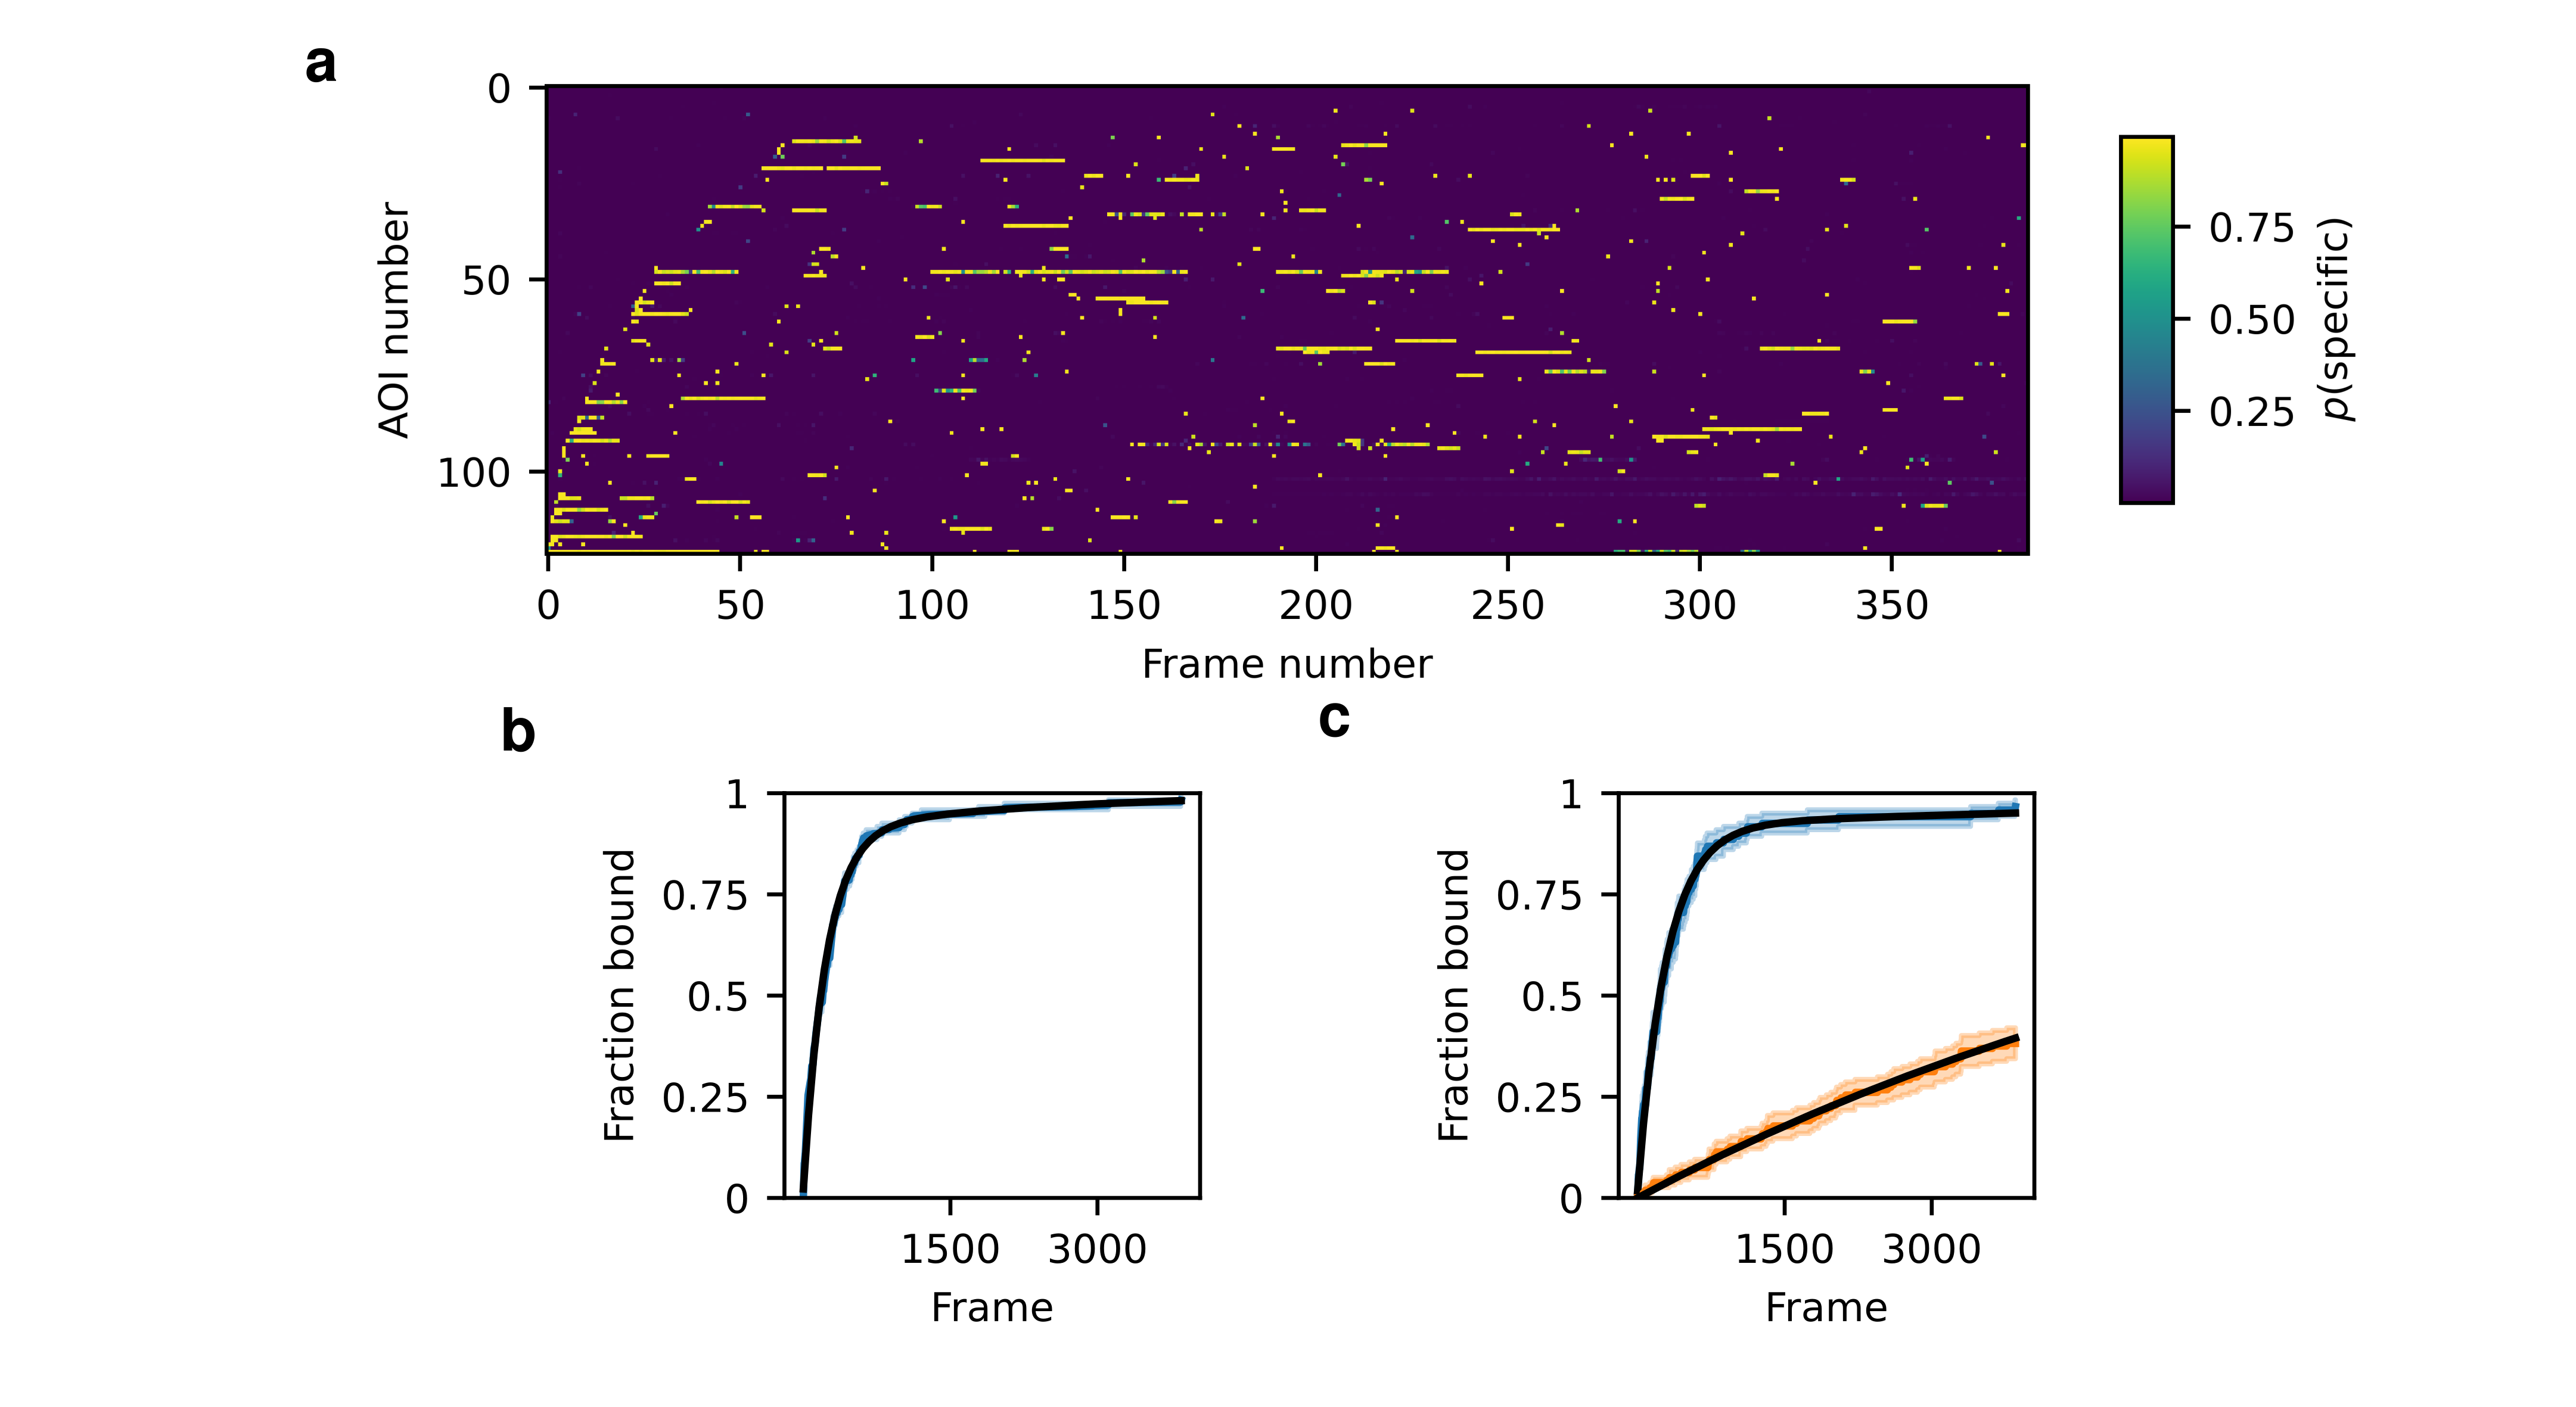
\includegraphics[width=\textwidth]{extended-data/figure4/figure4.png}
\caption{\textbf{Time-to-first binding analysis of experimental data.}  \textbf{a}, Rastergram representation of Tapqir-calculated target-specific spot  probabilities $p(\mathsf{specific})$ (color scale) for every 10\textsuperscript{th} frame of data at 122 different target locations.  AOIs were ordered by decreasing times-to-first-binding. Data set: $\sigma^{54}$RNAPCy3-598P2993 in Extended Data Table 1. \textbf{b,c}, Determining the association rate constant for the same data set by  time-to-first-binding analysis using Tapqir (\textbf{b}: $k_\mathrm{a} = 3.89 \: [3.44, 4.39] \times 10^{-3}$ s$^{-1}$, $k_\mathrm{ns} = 4.21 \: [1.67, 7.84] \times 10^{-4}$ s$^{-1}$, $A_\mathrm{f} = 0.905 \: []$) and an empirical spot-picker method (\textbf{c}: $k_\mathrm{a} = 3.28 \: [2.64, 4.05] \times 10^{-3}$ s$^{-1}$, $k_\mathrm{ns} = 1.3 \: [1.0, 1.6] \times 10^{-4}$ s$^{-1}$, $A_\mathrm{f} = 0.92 \: []$) \cite{Friedman2013-sf}. Cumulative fraction of target sites that exhibited one or more binding events by the indicated time (blue) and fit curve (black) yielding best-fit values for $k_\mathrm{a}$, $k_\mathrm{ns}$, and $A_\mathrm{f}$. Shading indicates 95\% confidence interval.
}
\label{fig:sigma54_298P2993}
\end{figure}
\clearpage
\pagebreak

\begin{table}[h]
\caption{\label{tab:datasets} \textbf{Experimental datasets.}}
% Use "S" column identifier to align on decimal point 
\begin{tabular}{lcrrrrr}
\toprule
Dataset & size & SNR & $\pi$ & $\lambda$ & $g$ & $\sigma^{xy}$ \\
\midrule
Rpb1\textsuperscript{SNAP549}-DNA\textsuperscript{488} & \begin{tabular}[x]{@{}c@{}}$N = 331$, $F = 790$\\$N_c = 526$, $F_c = 790$\end{tabular} & 1.61 &
0.114 & 0.320 & 6.44 & 0.575 \\
\midrule
$\sigma^{54}$RNAPCy3-598P2993 & \begin{tabular}[x]{@{}c@{}}$N = 122$, $F = 3855$\\$N_c = 157$, $F_c = 3855$\end{tabular} & 4.37 & $0.030$ & $0.0772$ & $16.91$ & $0.384$ \\
\midrule
$\sigma^{54}$RNAPCy3-597P255 & \begin{tabular}[x]{@{}c@{}}$N = 102$, $F = 4407$\\$N_c = 127$, $F_c = 4407$\end{tabular} & 3.87 & 0.073 & 0.149 & 11.414 & 0.448 \\
\bottomrule
\multicolumn{7}{l}{\footnotesize{\parbox{5in}{$N$ - number of on-target AOIs, $F$ - number of frames for on-target AOIs, $N_c$ - number of control off-target AOIs, $F_c$ - number of frames for off-target AOIs.}}} \\
\multicolumn{7}{l}{\footnotesize{\parbox{5in}{$^{1}$ Single molecule experiment measuring the binding rate of $\sigma^{54}$RNAP labeled with Cy3 to DNA where the target site for the polymerase on the DNA was bracketed different length (598P255) blue in Fig. 1E in \cite{Friedman2013-sf}}}} \\
\multicolumn{7}{l}{\footnotesize{\parbox{5in}{$^{2}$ Single molecule experiment measuring the binding rate of Rpb1\textsuperscript{SNAP549} to DNA\textsuperscript{488} \cite{Rosen2020-zn}}}} \\
\end{tabular}
\end{table}
\clearpage
\pagebreak

%\newcommand{\specialcell}[2][c]{%
%  \begin{tabular}[#1]{@{}r@{}}#2\end{tabular}}

% \multicolumn{6}{l}{\footnotesize{\parbox{0.9\textwidth}{$^{1}$For each dataset the first row is the randomized parameter value used in the simulation and the second row gives posterior predictions of parameter values and classification accuracy statistics. Each of the four parameters $\pi$, $\lambda$, $g$, and $\sigma^{xy}$ were independently and randomly selected from a broad range that encompasses typical experimental values. $N = 5$, $F = 500$, $N_c = 5$, $F_c = 500$, $h = 3000$, $w = 1.4$, $b = 150$, $\delta = 90$}}} \\
% \multicolumn{6}{l}{\footnotesize{\parbox{0.9\textwidth}{$^2$See Methods for SNR calculation.}}}


\begin{table}[h]
\caption{\label{tab:parameters} \textbf{Glossary of mathematical symbols.}}
\begin{tabular}{l l l}
\toprule
Symbol & Description & Domain \\
\midrule
$K$ & maximum number of spots per image & $\mathbb{N}$ \\
$N$ & number of AOIs & $\mathbb{N}$ \rule{0pt}{3ex} \\
$F$ & number of frames & $\mathbb{N}$ \rule{0pt}{3ex} \\
$P$ & number of pixels & $\mathbb{N}$ \rule{0pt}{3ex} \\
$g$ & camera gain & $\mathbb{R}_{>0}$ \rule{0pt}{3ex} \\
$\sigma^{xy}$ & proximity & $(0, (P+1)/\sqrt{12})$ \rule{0pt}{3ex} \\
$\pi$ & average target-specific binding probability & [0, 1] \rule{0pt}{3ex} \\
$\lambda$ & target-nonspecific binding rate & $\mathbb{R}_{>0}$ \rule{0pt}{3ex} \\
$\mu^b$ & mean background intensity across AOI & $\mathbb{R}_{>0}^{\mathsf{AOI}[N]}$ \rule{0pt}{3ex} \\
$\sigma^b$ & standard deviation of background intensity across AOI & $\mathbb{R}_{>0}^{\mathsf{AOI}[N]}$ \rule{0pt}{3ex} \\
$b$ & background intensity & $\mathbb{R}_{>0}^{\mathsf{AOI}[N] \times \mathsf{frame}[F]}$ \rule{0pt}{3ex} \\
$\theta$ & target-specific spot index & $\{0, 1, \dots, K \}^{\mathsf{AOI}[N] \times \mathsf{frame}[F]}$ \rule{0pt}{3ex} \\
$m$ & spot presence indicator & $\{ 0, 1 \}^{\mathsf{spot}[K] \times \mathsf{AOI}[N] \times \mathsf{frame}[F]}$ \rule{0pt}{3ex} \\
$h$ & integrated spot intensity & $\mathbb{R}_{>0}^{\mathsf{spot}[K] \times \mathsf{AOI}[N] \times \mathsf{frame}[F]}$ \rule{0pt}{3ex} \\
$w$ & spot width & $[0.75, 2.25]^{\mathsf{spot}[K] \times \mathsf{AOI}[N] \times \mathsf{frame}[F]}$ \rule{0pt}{3ex} \\
$x$ & center of the spot on the $x$-axis & $\mathbb{R}^{\mathsf{spot}[K] \times \mathsf{AOI}[N] \times \mathsf{frame}[F]}$ \rule{0pt}{3ex} \\
$y$ & center of the spot on the $y$-axis & $\mathbb{R}^{\mathsf{spot}[K] \times \mathsf{AOI}[N] \times \mathsf{frame}[F]}$ \rule{0pt}{3ex} \\
$\mu^S$ & 2-D Gaussian spot & $\mathbb{R}_{>0}^{\mathsf{spot}[K] \times \mathsf{AOI}[N] \times \mathsf{frame}[F] \times \mathsf{pixelX}[P] \times \mathsf{pixelY}[P]}$ \rule{0pt}{3ex} \\
$\mu^I$ & ideal image & $\mathbb{R}_{>0}^{\mathsf{AOI}[N] \times \mathsf{frame}[F] \times \mathsf{pixelX}[P] \times \mathsf{pixelY}[P]}$ \rule{0pt}{3ex} \\
$\delta$ & offset signal & $\mathbb{R}_{>0}^{\mathsf{AOI}[N] \times \mathsf{frame}[F] \times \mathsf{pixelX}[P] \times \mathsf{pixelY}[P]}$ \rule{0pt}{3ex} \\
$I$ & observed image w/o offset & $\mathbb{R}_{>0}^{\mathsf{AOI}[N] \times \mathsf{frame}[F] \times \mathsf{pixelX}[P] \times \mathsf{pixelY}[P]}$ \rule{0pt}{3ex} \\
$D$ & observed image & $\mathbb{R}_{>0}^{\mathsf{AOI}[N] \times \mathsf{frame}[F] \times \mathsf{pixelX}[P] \times \mathsf{pixelY}[P]}$ \rule{0pt}{3ex} \\
$x^\mathsf{target}$ & target molecule position on the $x$-axis & $[P/2-1, P/2]^{\mathsf{AOI}[N] \times \mathsf{frame}[F]}$ \rule{0pt}{3ex} \\
$y^\mathsf{target}$ & target molecule position on the $y$-axis & $[P/2-1, P/2]^{\mathsf{AOI}[N] \times \mathsf{frame}[F]}$ \rule{0pt}{3ex} \\
$i$ & pixel index on the $x$-axis & $\{0, \dots, (P-1)\}^{\mathsf{pixelX}[P]}$ \rule{0pt}{3ex} \\
$j$ & pixel index on the $y$-axis & $\{0, \dots, (P-1)\}^{\mathsf{pixelX}[P]}$ \rule{0pt}{3ex} \\
$D^\mathsf{raw}$ & raw microscope images & $\mathbb{R}_{>0}^{\mathsf{frame}[F] \times \mathsf{pixelX}[H] \times \mathsf{pixelY}[W]}$ \rule{0pt}{3ex} \\
$x^{\mathsf{target}, \mathsf{raw}}$ & target molecule position in raw images on the $x$-axis & $[-0.5, H-0.5]^{\mathsf{AOI}[N] \times \mathsf{frame}[F]}$ \rule{0pt}{3ex} \\
$y^{\mathsf{target}, \mathsf{raw}}$ & target molecule position in raw images on the $y$-axis & $[-0.5, W-0.5]^{\mathsf{AOI}[N] \times \mathsf{frame}[F]}$ \rule{0pt}{3ex} \\
\bottomrule
\end{tabular}
\end{table}
\clearpage
\pagebreak

\begin{table}[h]
\caption{\label{tab:dist} \textbf{Probability distributions used in the model.}}
\begin{tabular}{l l}
\toprule
Distribution & PDF \\
\midrule
$x \sim \mathbf{AffineBeta}(\mu, \nu, a, b)$ &
    $\dfrac{y^{\alpha-1}(1-y)^{\beta-1}}{\text{B}(\alpha, \beta)}$
    where $\alpha=\dfrac{\nu (\mu-a)}{b-a}$, $\beta=\dfrac{\nu (b-\mu)}{b-a}$, and $y = \dfrac{x-a}{b-a}$ \\
$x \sim \mathbf{Bernoulli}(\pi)$ &
    $\pi^x (1-\pi)^{1-x}$ \\
$x \sim \mathbf{Beta}(\alpha, \beta)$ &
    $\dfrac{x^{\alpha-1}(1-x)^{\beta-1}}{\text{B}(\alpha, \beta)}$ \\
$x \sim \mathbf{Categorical}_{\{z_i\}^k_{i=1}}(\mathbf{p})$ &
    $\prod_{i=1}^k p_i^{[x=z_i]}$ \\
$x \sim \mathbf{Gamma}(\mu, \sigma)$ &
    $\dfrac{\beta^\alpha}{\Gamma(\alpha)}x^{\alpha-1} e^{-\beta x}$
    where $\alpha = \dfrac{\mu^2}{\sigma^2}$ and $\beta = \dfrac{\mu}{\sigma^2}$ \\
$x \sim \mathbf{HalfNormal}(\sigma)$ &
    $\dfrac{\sqrt{2}}{\sigma \sqrt{\pi}} \exp \left( -\dfrac{x^2}{2\sigma^2} \right)$
    for  $x > 0$ \\
$k \sim \mathbf{TruncatedPoisson}(\lambda, K) $ & $ \begin{cases} 1 - e^{-\lambda} \sum_{i=0}^{K-1} \dfrac{\lambda^i}{i!} & \textrm{if $k = K$} \\ \dfrac{\lambda^k e^{-\lambda}}{k!} & \textrm{otherwise} \end{cases} $ \\
$x \sim \mathbf{Uniform}(a, b)$ &
    $\dfrac{1}{b-a}$ for $x \in [a, b]$ \\
\bottomrule
\end{tabular}
\end{table}

\end{document}

% Multi-wavelength single-molecule fluorescence colocalization methods allow elucidation of complex biochemical reaction mechanisms. However, analysis of colocalization data is an intrinsically challenging and time-consuming problem for multiple reasons. First, to minimize dye photobleaching, images frequently are collected at low signal-to-noise ratios, making it challenging to discriminate real fluorescent spots from noise. Second, transient non-specific interactions of the binder molecule with the surface of the microscope slide can give rise to both false-positive and false-negative detection. Third, current analysis methods require subjective choice of user-set thresholds for such spot parameters as amplitude, diameter and proximity. To overcome these difficulties, we developed a new analysis method based on statistical modeling of the image data. This method: 1) maximizes extraction of useful information from data by analyzing 2-D images, not integrated intensity; 2) discriminates authentic fluorescence spots from fluctuations in background fluorescence in a probabilistic manner and assigns spot probabilities (not merely a binary "spot/no spot" classification); 3) uses a realistic pixel intensity model that accounts for background, spot, and camera noise sources; 4) explicitly models non-specific interactions of binder molecules with the slide surface; and 5) can globally fit data from experimental samples together with negative controls that lack target molecules. The software is implemented in the Python-based Pyro probabilistic programming language, which incorporates modern deep machine learning and Bayesian modeling to allow easy substitution of different statistical models, efficient use of parallelized processing (GPU) hardware, and scalability to large data sets. The algorithm is effective without manual parameter tweaking on both simulated and experiment-derived data sets with a wide range of signal, noise, and non-specific binding characteristics. We anticipate that this work will increase the accessibility and utility of single-molecule fluorescence colocalization methods.